% !Mode:: "TeX:UTF-8"
\documentclass[preprint,authoryear,PhD]{cumtthesis}
\usepackage{listings}
\usepackage{multirow}
%\usepackage[left=3.17cm,right=3.17cm,top=3.0cm,bottom=3.0cm]{geometry}

%=================================== 数学符号 =================================%
\newcommand{\rtn}{\mathrm{\mathbf{R}}}
\newcommand{\N}{\mathrm{\mathbf{N}}}
\newcommand{\AS}{~\mathrm{a.s.}}
\newcommand*{\PR}{\mathrm{\mathbf{P}}}
\newcommand*{\EX}{\mathrm{\mathbf{E}}}
\newcommand*{\dif}{\,\mathrm{d}}
\newcommand*{\F}{\mathcal{F}}
\newcommand*{\prs}{\dif\PR-\mathrm{a.s.}}
\newcommand*{\pts}{\dif\PR\times\dif t-\mathrm{a.e.}}
\newcommand{\Ito}{It\^{o}}
\newcommand{\tT}[1][0]{[#1,T]}
\newcommand{\intT}[2][T]{\int^{#1}_{#2}}
\newcommand{\s}{\mathcal{S}}
\newcommand{\me}{\mathrm{e}}
\newcommand{\one}[1]{{\bf 1}_{#1}}
\newcommand{\Mm}{{\rm M}}
\DeclareMathOperator*{\sgn}{sgn}
%=================================== 数学符号 =================================%

\makeindex

\begin{document}
\frontmatter

%--------输入中文论文题目
\CLunWenTiMu{中国矿业大学硕博毕业论文 \LaTeX{} 模板 V2.0 (2015/08/04)}

%--------输入英文论文题目
\ELunWenTiMu[0.95]{China University of Mining and Technology \LaTeX{} Thesis Template V2.0 (2015/08/04)}

%--------输入论文作者
\ZuoZhe{肖立顺}

%--------输入导师职称,导师姓名
\DaoShi[教授]{范胜君}
\DiErDaoShi[教授]{江龙}

%--------输入毕业时间
\BiYeShiJian{2013}{10}

%--------输入中图分类号
\ZhongTuFenLeiHao{O211.5}

%--------输入UDC
\UDC{519.2}

%--------输入密级
\MiJi{公开}

%--------输入毕业学校, 默认是中国矿业大学
%\BiYeXueXiao{}

%--------输入学校代码, 默认是10290
%\XueXiaoDaiMa{}

%--------输入学位类别
\XueWeiLeiBie{理学}

%--------输入培养单位
\PeiYangDanWei{理学院}

%--------输入学科专业
\XueKeZhuanYe{概率论与数理统计}

%--------输入研究方向
\YanJiuFangXiang{随机分析}

%--------输入答辩委员会主席
\DaBianWeiYuanHuiZhuXi{江龙}

%--------输入评阅人
\PingYueRen{江龙, 周圣武}

%--------制作封面命令
\makecover

%--------致谢
\begin{acknowledgements}
  从 2011 年开始制作 cumtthesis.cls 的第一个版本, 到 2015 年的 V2.0 版本, 花费了大量的时间和精力, 期间得到了很多好心人的帮助.

  编写 cumtthesis.cls 中图表清单的代码时, \href{http://tex.stackexchange.com/}{酷 \LaTeX{} 问答站} 的 egreg
  帮我解决了关键性的技术问题, 并且很耐心很及时地解答我的疑问.

  我是看了薛瑞尼制作的 thuthesis.dtx 源代码才开始琢磨如何``文学式"编程. 从薛瑞尼的代码和
  文档中, 我得到了很多启发. 比如图表标题的制作, 比如变量注释表的代码编写, 还比如
  \verb|*.dtx| 文档的制作等.

  cumtthesis.cls 中双语目录的编写受哈尔滨工业大学硕博士学位论文 \LaTeX{} 模板 (1.9.2.20090324 版) 的启发,
  通过 \verb|*.toe| 文件来生成英语目录.

  第 \ref{cha:IntroductionOfTeX} --  \ref{cha:ResumesOfSupermans} 章的演示内容复制于
  \href{http://zzg34b.w3.c361.com/}{\LaTeX{} 编辑部}.
\end{acknowledgements}

%--------中文摘要
\begin{cabstract}
本文是对 cumtthesis.cls 模板的演示, 体现模板的各种功能. 制作 cumtthesis.cls
的目的是给矿大学子提供一个简洁易用的毕业论文模板, 宗旨是让使用者只关心论文的内容
而不用关心论文的格式.

本文总共有图 \ref{totalfigure} 幅, 表 \ref{totaltable} 张, 参考文献 \ref{totalbib} 篇.

%--------中文关键词
\CKeyWords{
\LaTeX; 模板; 中国矿业大学; 硕博论文; Word; 宏包;
cls 文档; 代码; 默认格式; 参考文献; 双语标题; 双语目录; 页面边距; 定理;
定义; 交叉引用.}
\end{cabstract}

%--------英文摘要
\begin{eabstract}
This paper is an illustration of cumtthesis.cls, which can reflect the various
functions of the template. The purpose of cumtthesis.cls is to provide a
simple and easy-to-use thesis template for cumters. It allows users to only
care about the content of the papers rather than the format.

There are totaly \ref{totalfigure} figures, \ref{totaltable} tables and \ref{totalbib} references
in this paper.

%--------英文关键词
\EKeyWords{\LaTeX; CUMT; Thesis of MD and PhD; Word; Package; cls document;
Codes; Default format; References; Bilingual titles; Bilingual contents;
Page margins; Theorem; Definition; Cross reference.}
\end{eabstract}

%-------英文拓展摘要
\begin{exabstract}
This paper is an illustration of cumtthesis.cls, which can reflect the various
functions of the template. The purpose of cumtthesis.cls is to provide a
simple and easy-to-use thesis template for cumters. It allows users to only
care about the content of the papers rather than the format.

There are totaly \ref{totalfigure} figures, \ref{totaltable} tables and \ref{totalbib} references
in this paper.

%--------英文拓展关键词
\ExKeyWords{\LaTeX; CUMT; Thesis of MD and PhD; Word; Package; cls document;
Codes; Default format; References; Bilingual titles; Bilingual contents;
Page margins; Theorem; Definition; Cross reference.
}
\end{exabstract}




%--------插入中文目录
\tableofcontents
%--------插入英文目录
\tableofecontents

%--------插入图清单
\listoffigures
%--------插入表清单
\listoftables
%--------变量注释表

\begin{notation}[2.5cm]
\item[$P$] 概率
\item[$\mathcal{F}$] 域流
\item[cumtthesis.ins] 模板的分解文件
\item[cumtthesis.dtx] 模板的说明文件
\item[cumtthesis.pdf] 模板的使用说明
\item[cumtthesis.cls] 模板的文档类
\item[cumtthesis.cfg] 文档类的配置文件
\item[cumt.bst] 矿大参考文献样式
\item[.tex] 示例文档代码
\item[.pdf] 示例文档
\item[.aux] 引用标记记录文件, 用于再次编译时生成参考文献和超链接等
\item[.bbl] 由 BibTeX 编辑 .bib 后创建的文献文件, 再次编译时带入源文件生成文献列表
\item[.blg] BibTeX 处理过程记录文件
\item[.dvi] 由 \LaTeX{} 对 .tex 源文件编译后创建的输出文件, 含有字库信息
\item[.glo] 术语标记记录文件, 用于再次编译时生成术语表
\item[.idx] 索引资料记录文件, 可用 makeindex 排序后创建索引文件 .ind
\item[.ilg] makeindex 处理过程记录文件
\item[.ind] makeindex 对 .idx 排序后创建的索引文件, 再次编译时带入源文件生成索引
\item[.lof] 图形标题记录文件, 用于再次编译时生成图形目录
\item[.log] 编译过程记录文件, 记录编译时出现的提示, 警告和错误信息
\item[.lot] 表格标题记录文件, 用于再次编译时生成表格目录
\item[.toc] 中文章节标题记录文件, 用于再次编译时生成中文章节目录
\item[.toe] 英文章节标题记录文件, 用于再次编译时生成英文章节目录
\item[\bf 英雄本色] 我等这个机会等了三年, 不是为了证明我比别人强, 只是要证明我失去的
    东西, 我一定要夺回来.
\item[\bf 临江仙 (杨慎)]滚滚长江东逝水, 浪花淘尽英雄, 是非成败转头空, 青山依旧在, 几度
    夕阳红. 白发渔樵江渚上, 惯看秋月春风. 一壶浊酒喜相逢, 古今多少事, 都付笑谈中.
\item[\bf 大话西游] 曾经有一份真诚的爱情摆在我的面前, 我没有珍惜, 等到失去的时候才追悔
    莫及, 人世间最痛苦的事情莫过于此. 如果上天能够给我一个重新来过的机会, 我会对那
    个女孩子说三个字:``我爱你". 如果非要给这份爱加上一个期限, 我希望是, 一万年.
\item[\bf 喜剧之王] 你可以说我是跑龙套的, 但是你不可以说我是``臭跑龙套"的.
\item[\bf 东邪西毒] 当你不能够再拥有, 你唯一可以做的, 就是令自己不要忘记.
\item[\bf 纵横四海] 其实爱一个人并不是要跟她一辈子的. 我喜欢花, 难道你摘下来让我闻;
    我喜欢风, 难道你让风停下来; 我喜欢云, 难道你就让云罩着我; 我喜欢海, 难道我就去
    跳海?
\item[\bf 无间道] 往往都是事情改变人, 人却改变不了事情.
\item[\bf 笑傲江湖] 有人就有恩怨, 有恩怨就有江湖. 人就是江湖, 你怎么退出!
\item[\bf 泰坦尼克号] 我甚至连他的一张照片都没有, 他只活在我的记忆里.
\item[\bf 似水年华] 一个男人和一个女人, 他们在完全对对方没有任何了解和认识的情况下,
    竟然会在一个清晨, 拥抱在一起. 他们在渴求的是什么? 他们不是在要对方, 他们在要自
    己. 我们在所有经过的爱情当中, 都不是看到的对方, 只是看到了自己.
\end{notation}

%================================== 正文开始 ==================================%
\mainmatter

\chapter{绪论}{Introduction}
\section{研究背景和意义}{Background and Research Significance}
智慧城市是由数字城市、物联网和云计算三大类支撑技术组成,其中数字城市是智慧城市的核心,
主要包含天地空一体化空间信息快速获取、海量空间数据管理、空间信息可视化技术、空间数据分析挖掘和
网络服务技术\cite{李德仁2013智慧地球时代测绘地理信息学的新使命}。互联网尤其移动互联网的快速发展,
使得数字城市面临巨大的挑战:空间数据获取手段不再局限于传统人工测量,基于用户地理位置服务(Location Based Service, LBS)
功能使得网络中包含了用户的空间数据;每天产生的海量数据对数据存储、索引和查询提出高性能要求;
海量空间数据使得空间知识愈发贫乏,急需海量空间数据挖掘相关研究。

相关调查表明,中国大陆是全球移动互联网用户最多的地区,移动互联网设备上各种APP记录了每个用户生活的
方方面面,比如打车软件记录城市居民出行数据,O2O软件反映了城市线下商圈服务区域情况。其中以新浪微博为代表
的社交网络应用最为值得研究,超过一大半移动互联网用户都拥有新浪微博账号。作为高频使用应用程序,
新浪微博已经成为数字城市空间数据不可忽视的重要数据来源。在社交网络中,用户的行为往往是自发进行的,这些数据蕴含了城市居民
生活的真实信息,快速精确的对这些数据进行空间书分析和挖掘对智慧城市建设有着重大意义,主要包含
以下三个方面:

(1)对个人而言,对网络空间数据挖掘,可以发现不同的知识,为生活带来便利,如交通路线规划、旅游景点推荐等,构建城市智慧生活。

(2)对商业公司而言,通过空间数据挖掘发现目标客户使用习惯或群体性活动规律,对商业推广计划提出指导性意见,如广告投放、精准营销等,
是城市智慧商业重要组成部分。

(3)对政府决策部门而言,城市居民的社交网络中的行为是社会现实现象的反映,能够发现社会的经济、文化、交通等众多方面活动规律。为智慧城市
发展的各项决策提供建议。

智慧城市提出了海量空间数据高效处理的需求,目前针对海量数据普遍采用分布式并行计算,其核心思想是将海量数据划分
为若干个子集,将每个子集分配给不同的线程、进程或者是机器进行并行处理,最后将每个子集计算出来的结果进行合并,得到全局计算结果。
Hadoop MapReduce\cite{Shvachko2010The}是业界广泛使用的并行分布式计算框架,通过对数据处理过程的高度抽象,
使普通开发人员编写分布式并行计算成为可能。但是现实业务需求的更迭,这些计算框架面对迭代计算需求显得捉襟见肘,
Spark作为新一代的开源通用并行计算框架\cite{Zaharia2010Spark},大大扩展了MapReduce表现能力,
而且通过内存计算独特的运行机制,避免了IO操作,使得Spark更好适应数据挖掘和机器学习等一些迭代算法\cite{李文栋2015基于}。
但Spark在处理空间数据的时候,其抽象程度仍然较低,不支持空间数据类型表达和空间数据运算,
因此高效海量空间数据并行计算框架的需求迫在眉睫,空间分析和空间数据挖掘算法并行化设计也值得进一步研究。

\section{国内外研究现状}{Research Progress at Home and Abroad}
\subsection{并行计算框架研究现状}
自$2004$年Google公司公布分布式并行计算框架思想后\cite{Dean2004MapReduce},开源分布式并行计算框架Hadoop被业
界广泛使用,其效仿GFS(Google File System)设计思想,提出了HDFS(Hadoop Distributed File System)分布式文件系统,
同时也提供MapReduce编程模型,该计算模型简单,适合大规模数据分析。以Hadoop为核心,发展出完整的大数据处理分析技术生态圈,
如非关系型数据库HBase\cite{Lars2011HBase},机器学习库Mahout\cite{Lyubimov2016Apache},资源管理
平台YARN\cite{Vavilapalli2013Apache}等等。整个技术生态圈在开源社区中不断完善,在生产实际中广泛使用。

随着业务场景的不断改变,Hadoop MapReduce的缺陷越来越被用户所诟病,UC Berkeley AMP实验室提出Spark并行计算框架,并以
弹性分布式数据集(RDD)为核心提出一套完整的技术栈。与MapReduce相比该计算框架
的特点在于内存计算,避免了中间数据的IO操作,RDD还提供一系列丰富的操作算子\cite{Zaharia2010Spark},使之表现
能力大大提高。Spark支持多种编程语言,除了开发语言Scala,还支持传统的Java和脚本语言Python,也支持统计语言R。与Hadoop MapReduce
只能编写Jar包提交程序不同,Spark还提供类似Shell的交互式编程方式,通过即时反馈快速搭建算法原型,提高开发效率。

Spark一经推出,受到了学术界和工业界广泛关注,学术界对Spark源码进行改进,使之更加稳定,增加新的功能,截止目
前Spark版本已经发展到$2.0$版本,在GitHub上已超过一千名开发者参与。工业界也在广泛使用Spark来处理业务逻辑,
有些商业公司也还推出商业并行计算云平台\cite{2015Aliyun, Varia2011Best},将并行计算资源向整个社会开放。用户
根据需求购买相应的虚拟机资源,该资源能够快速完成并行计算运行环境配置,省去了用户搭建计算平台等复杂的工作。

\subsection{并行计算空间数据分析研究现状}   
近年来,伴随着并行计算框架的提出,国内外学者做了大量并行计算环境下的空间分析的研究。

马磊在HDFS上分级建立R树空间索引\cite{马磊2016一种基于},加快海量空间数据查询速度;方金云等人根据空间查询特性和
Spark分布式内存计算模型\cite{方金云2015基于},设计HBase分布式存储Spark分布式内存计算框架的空间区域查询算法;
温馨实现一种基于Shark/Spark的分布式空间数据分析框架\cite{温馨2015基于},通过自定义函数和空间函数下推两种实现
空间查询方式;李璐明,蒋新华等人使用Spark对海量空间数据进行密度聚类\cite{李璐明2015基于弹性分布数据集的海量空间数据密度聚类},
并根据Spark并行计算特点提出了并行密度聚类算法PClusterdp;靳凤营,张丰等对矢量空间数据,使用
Spark进行空间叠加分析,性能与传统Oracle+ArcSDE两种方法进行发现Spark在处理海量中有较大的优势\cite{靳凤营2016基于}。

Abouzeid A.将分布式技术和关系型数据结合进行一些尝试\cite{Abouzeid2009HadoopDB},使用MapReduce
管理多个数据库,转换HadoopDB中的SQL语句,将操作推入到数据库层处理;Witayangkurn A.和Horanont T.等人将Hadoop-GIS与
Hive相结合,实现MapReduce处理边界对象\cite{Witayangkurn2012Performance};美国环境系统研究所(ESRI)开发
Esri Geometry API for Java和Spatial Framework for Hadoop,将ArcGIS向Hadoop拓展,通过在Hive中自定义空间查询
函数进行空间数据查询\cite{ESRIGIS};Nathan K.在Hadoop平台上使用了MapReduce并行计算框架对比分析处理,并对比
Hadoop云计算平台和传统的单节点价格的PostGIS空间数据库进行分析处理;Ahmed E.和Mohamed F.M.提出SpatialHadoop框架
,通过改进Hadoop源码,增加了空间数据处理的支持,如空间数据类型、空间操作、空间查询和空间过滤\cite{Eldawy2016SpatialHadoop};
Jia Y.,JinXuan W.和Mohamed S.等人尝试了在Spark上处理空间数据,对比了Spark与SpatialHadoop空间计算性能\cite{Yu2015GeoSpark}。

综合文献资料,可以了解到国内外学者对大数据计算框架在空间数据处理中的应用逐渐增多。从原先的MapReduce计算框架向Spark
计算框架进行迁移;数据存储由传统的关系型数据库向key-value非关系型数据库转变;数据格式从常用的Shapefile文件向WKT,JSON等文本型数
据格式转变。但是这些试探性研究尚未能够将空间数据类型和空间数据分析纳入到Spark计算体系中,并空间数据挖掘算法向并行化重新设计研究较少。

\subsection{微博空间数据研究现状}
国内外学者很早就注意到社交网络中包含了巨大的研究价值,Andrienko G.和Andrienko N.等人通过研究Twitter(类似新浪微博)中的推文分析
美国西雅图人们每天生活习惯模式\cite{Andrienko2013Thematic};Linna L.和Michael F.通过结合Twitter和Flickr(图片社交
网站)分析社交网络在空间、时间和经济方面的发展状况\cite{Linna2013Spatial};Hollenstein L.和Purves R.通过带有地理标签的Flickr
图片分析人们在现实世界中活动规律\cite{Hollenstein2010Exploring};Xingjian L.和Jianghao W.通过带有地理位置的新浪微博,分析国内和
海外用户分布特征\cite{Liu2015The};刘大均,胡静等人根据新浪微博旅游版块分析中国旅游空间分布格局和影响因素\cite{刘大均2015中国旅游微博空间分布格局及影响因素};
徐艳等人通过手动筛选新浪微博用户关系数据分析重庆市城市网络空间特征分布\cite{徐艳2014基于新浪微博视角下的城市网络空间特征分析——以重庆市主城区为例}。

从上述研究现状中可以看出,目前对社交网络中空间信息探索研究越来越得到重视,通过线上数据发现线下真实状况具有较强的现实意义,然而目
前基于新浪微博研究存在样本量较小,选择片面性和数据存在人工干预等不足,如何通过类「全样本」新浪微博空间数据分析,从宏观角度发现
有价值的信息对现实有着重要的指导意义。

\section{研究内容和技术路线}{Contents of Research and Technology Route}
\subsection{研究内容}
本文将从数字城市对海量空间数据高效处理需求出发,研究Spark并行计算框架的核心内容,对Spark RDD进行空间扩展,使之
能够支持空间数据类型和空间分析。

以此计算框架为基础,将串行的空间数据挖掘算法并行化改进,以海量新浪微博POI和用户位置数据进行空间数据分析和挖掘。
主要研究内容如下:

(1)分析现有的开源分布式计算框架MapReduce和Spark工作机制,并比较了各自的优缺点;

(2)分析新浪微博空间数据获取接口,编写新浪微博空间数据的应用程序;

(3)对Spark RDD进行空间扩展,开发Spatial-Spark并行计算框架,使该框架支持点、线和面基本空间几何对象和空间索引建立,
在此基础上提供常用的并行化空间分析运算接口;

(4)以Spatial-Spark为基础,对新浪微博POI数据进行并行化空间模式挖掘;

(5)使用Spatial-Spark对新浪微博用户位置信息构建人口流动网络图,分析城市人口流动量、城市网络权重和设计并行化社群挖掘算法。

\subsection{技术路线}
从Spark RDD空间扩展出发,对空间数据的点、线和面分别形成PointRDD、LineRDD和PolygonRDD,
并分区建立空间索引,在此基础上提供并行化空间拓扑查询、空间KNN查询和空间连接查询等空间分析
操作,构建并行空间计算框架Spatial-Spark。

对全国的新浪微博POI数据和新浪微博用户位置数据,使用Spatial-Spark对海量的空间数据进行数据分析,主要包括统计分析、
同位模式挖掘、权重分析和社群挖掘。本文的技术路线见图\ref{fig:thetechroute}。
\begin{sidewaysfigure}
\centering
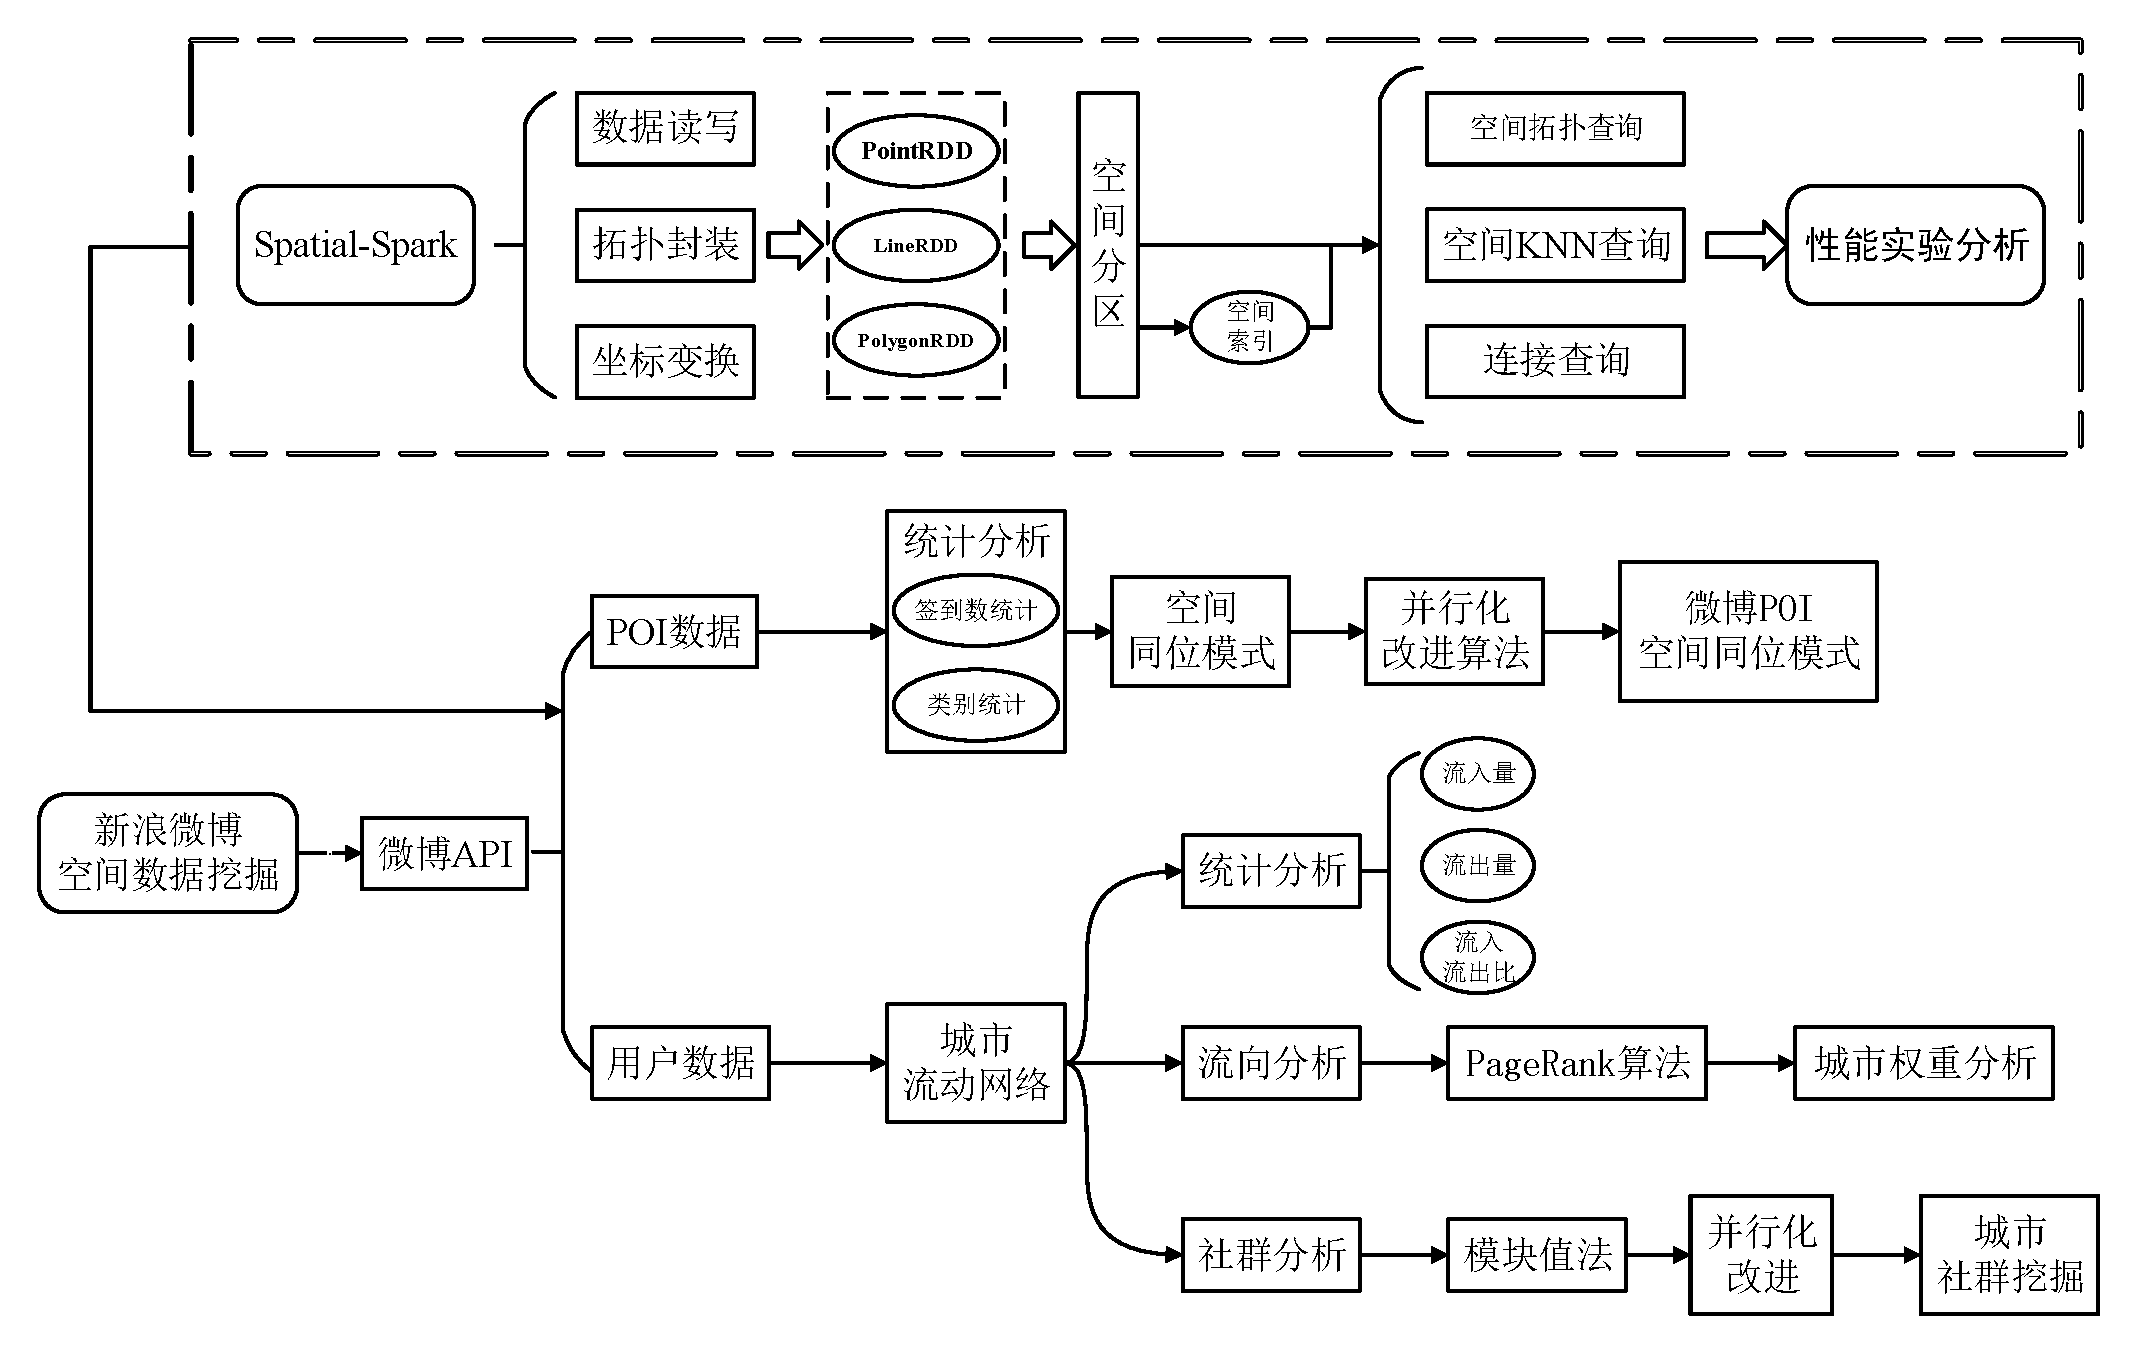
\includegraphics[height=14cm]{figures/technology_route.pdf} \\
\caption{技术路线}{Technology route}
\label{fig:thetechroute}
\end{sidewaysfigure}

\section{论文结构安排}{Contents and Structure of This Thesis}

第一章:绪论。 概要地说明了论文的研究背景及意义和国内外相关主题研究现状,
阐述了本文的工作,以及论文的主要内容和技术路线。

第二章:相关技术。重点介绍了Spark并行计算框架,空间数据挖掘相关算法和新浪微博API接口。

第三章:Spatial-Spark计算框架。设计了Spatial-Spark计算框架,对空间数据的支持,空间索引的建立和空间运算,
最后用实验比较Spatial-Spark在空间分析方面的优势。

第四章:新浪微博POI数据分析。主要包括类别统计分析和POI类别空间同位模式挖掘。

第五章:新浪微博用户流动网络分析。主要包括人口流动量统计、城市权重分析和网络社群挖掘。

第六章:总结与展望。对论文的研究内容和成果进行总结,指出了研究内容的局限性并对后期工作提出建议。

\chapter{相关技术}{Related Technology}
\section{Hadoop技术}{Hadoop Technology}
自从Google公司公布分布式计算三架马车MapReduce、GFS和BigTable之后,Apache基金会开放了
Hadoop大数据计算平台,并发展成为Apache顶级项目,包含了Google公司三架马车的开源实现,分别为
Hadoop MapReduce、HDFS和HBase。Hadoop一经推出备受开源社区广泛关注,其拥有较高的容错性、可靠性和适用性等
优点,最重要的是Hadoop可部署在廉价的普通PC机器上,大大降低开发成本。Hadoop MapReduce是Hadoop的计算
模型,该模型将所有数据处理流程分解为Map阶段和Reduce阶段\cite{Dean2004MapReduce},这个计算模型的优势
在于使用简单,它隐藏了并行化、容错、位置优化和负载均衡的细节,使得没有并行和分布式经验的开发人员能够处理业务逻辑,
这也是Hadoop成为大数据计算框架被广泛关注和研究的原因。

\subsection{HDFS机制}

HDFS是Hadoop分布式计算框架中数据存储基础,同其他分布式文件系统PVFS(Parallel Virtual File System)、
Lustre和GFS一样,HDFS将系统元数据存储在特定的节点上,称之为NameNode;应用程序所需数据存储在其余的节点上,
称之为DataNode。为了保证容错性,需要指定特定节点作为SecondaryNameNode,它是NameNode的备用节点,负责
拉取主控服务器的日志。当NameNode发生失效,替代原来的NameNode的进行工作,所有节点使用TCP协议进行连
接和通信\cite{Shvachko2010The}。

HDFS采用主从结构,集群一般由一个NameNode和多个DataNode组成。不同于PVFS和Lustre的RAID(Redundant Array of 
Independent Disks)文件保护机制,HDFS将数据文件切分成若干数据块(Block),默认为64M,将这些文件分散到不
同DataNode节点并且每个数据块拷贝若干份,通过这些措施来提高数据的可靠性,图\ref{fig:hdfsarchitecture}为HDFS体
系结构。
\begin{figure}
\centering
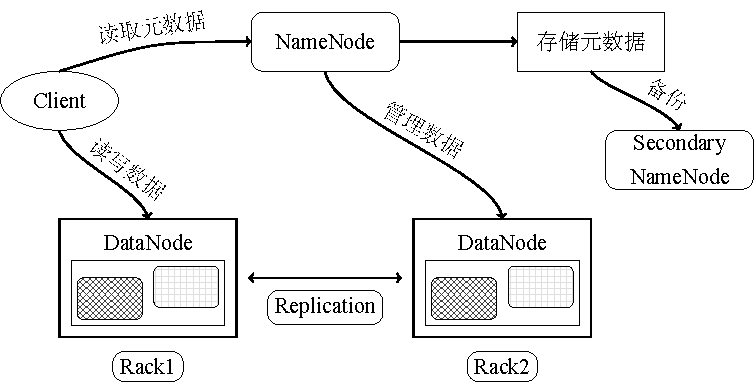
\includegraphics[width=0.9 \linewidth]{figures/hdfs.pdf}
\caption{HDFS体系结构}{HDFS architecture}
\label{fig:hdfsarchitecture}
\end{figure}

HDFS对数据的操作主要表现为数据的读写和数据块的备份:

数据读写操作:当客户端(Client)向NameNode发起读取数据请求,NameNode通过元数据判断该数据存在,如果存在,HDFS将返回该
数据所在的详细位置给客户端。客户端将使用TCP协议与数据对应的DataNode进行通信读取数据;数据写入的过程与之稍微不同,
客户端同时向NameNode和DataNode发送请求,当NameNode接收到来自DataNode的消息立即返回确认消息,DataNode开始进行数据
写入。

数据块备份操作:对于较大的集群,由于DataNode众多,不可能同时管理Block。通常将将这些Block分布在不同的机架上,
机架内部通信带宽往往比机架间大得多。因此通过NameNode接受来自DataNode的心跳和Block的报告,将Block备份到不同
的节点和机架上\cite{Oriani2012From}。

\subsection{MapReduce编程模型}

Hadoop MapReduce是Google MapReduce开源实现,其核心思想则是源于函数式编程语言。它将分布式业务逻辑从
复杂的细节中抽象出来,开发人员只需要关注Map函数和Reduce函数便可以通过集群系统来执行程序,实现分布式计算,而
无需关注消息传递和计算任务分配等复杂的问题。

Map阶段关注的是任务的分解,通过Map算子将每个输入输出组成Key/Value键值对作为输入和输出形式。Reduce算子是
对Map算子的输出进行汇总,以Key按照特定的分区算法,并行执行Reduce函数。

以Word Count任务为例,MapReduce运行机制见图\ref{fig:mapreduce},按照执顺序包括:输入分片(Input Split)、Map阶段、Shuffle阶
段和Reduce阶段\cite{SinghMapReduce}。
\begin{figure}
    \centering
    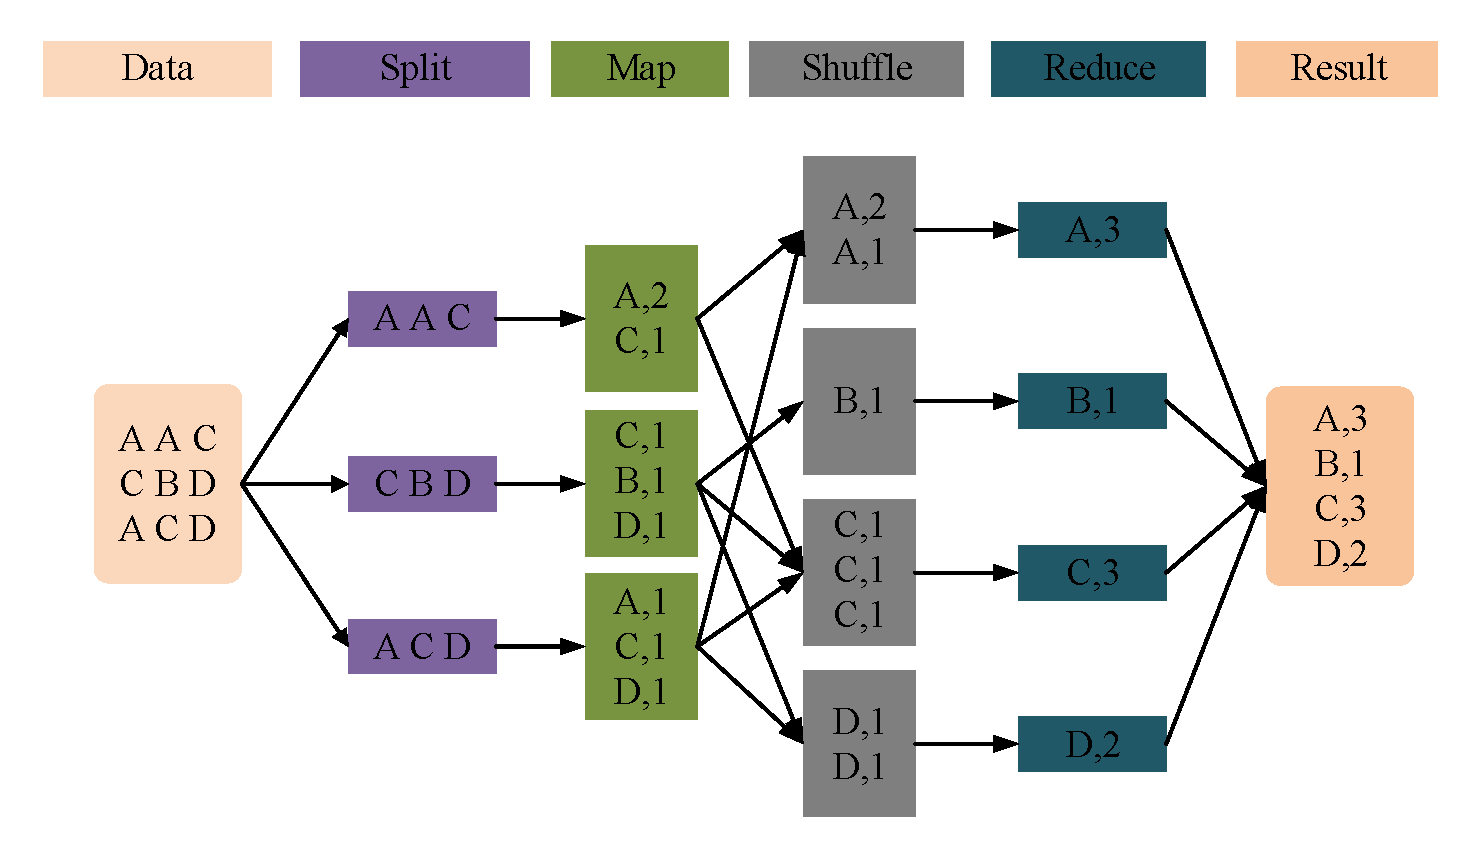
\includegraphics[width=0.8 \linewidth]{figures/mapreduce.pdf} \\
    \caption{Word-Count处理流程}{Word-Count procession}
    \label{fig:mapreduce}
\end{figure}

(1)输入分片:在进行Map计算之前,MapReduce会根据输入数据计算输入分片,每个输入对应着一个Map任务,输入分片和HDFS
数据文件的Block相关,即每个输入数据文件是HDFS默认大小的整数倍,不满整数向上取整。如果存在较多的小文件,将会
导致Map执行阶负载不均衡。

(2)Map阶段:开发人员重写Map函数,以满足特定的业务逻辑需求,而且Map函数一般在数据所在节点执行,从而降低了通信消耗时间。

(3)Shuffle阶段:Map阶段到Reduce阶段之间过程就是Shuffle过程,也是MapReduce性能提升的重点地方。MapReduce计算
的是海量数据,内存中不可能存储所有数据,Map阶段在输出时会将部分数据写入磁盘,等Map输出所有数据后,Map会采用
类似归并排序(Merge Sort)算法对输出结果合并。这个过程中会有一个Partitioner操作。每个Partitioner操作对应
一个Reduce作业,Partitioner就是Reduce阶段输入分片,开发人员可以编写Partitioner函数,提高Reduce阶段执行效率。

(4)Reduce阶段:对来自Shuffle阶段的输入数据进行汇总处理,开发人员根据业务需求,自行编写Reduce函数,并将结果数据
存储在HDFS上。
\subsection{MapReduce不足}
在Hadoop$1.0$版本中,MapReduce框架有唯一的Master、JobTracker和每个集群节点一个Slaver、TaskTracker共同组
成。其缺点显而易见,JobTracker是MapReduce的集中处理节点,存在单点故障的风险;JobTracker完成了太多的任务,造
成了过多的资源消耗等。在Hadoop$2.0$版本中,推出了YARN(Yet Another Resource Negotiator)统一的资源管理平台,该
平台能够很好地将不同的任务隔离开来,增加集群的健壮性。

虽然MapReduce通过高度抽象,能够很好地描述大部分业务逻辑,但还是过于底层。简单的过滤(Filter),分组(Group by)等
操作都需要编写冗长的Map和Reduce接口函数,无形中增加了开发人员的负担和出现故障的概率\cite{Grolinger2014Challenges}。
而且整个流程中的中间过程数据都要缓冲到HDFS中,磁盘IO时间开销都是系统性能的瓶颈,尤其是针对数据挖掘、机器学习等需要
反复迭代的算法,MapReduce编程模型往往是捉襟见肘。

\section{Spark计算框架}{Spark Framework}
Spark作为炙手可热开源并行计算框架,吸收和借鉴了MapReduce思想,并提出了新型的内存计算模型,将整个计算过程中数据保存在
集群内存中,从而大大提高了Spark表现力。Spark同样隐藏了并行化的细节,使用者只需要关心业务需求。
\subsection{Spark框架体系}
BDAS(the Berkeley Data Analysis Stack)是AMP实验室打造的一个开源的大数据处理一体化的技术生态系统,见图\ref{fig:sparkarchitecture},
整个生态主要分为三大部分,核心部分为Spark Runtime支持的Spark Core,其包含了Spark最基本、最核心的功能和基本分布式并行
计算算子,这些算子提供了Java,Scala,Python和R编程语言接口。在上层部分是为处理特定业务场景而设计的生态组件,是Spark的高层组件,
分别为:结构化查询工具Spark SQL、分布式机器学习库MLlib、并行图计算框架GraphX和流计算框架Spark Streaming。
底层为集群管理器,如YARN,Mesos等等,保证了Spark运行框架运行的健壮性。
\begin{figure}
\centering
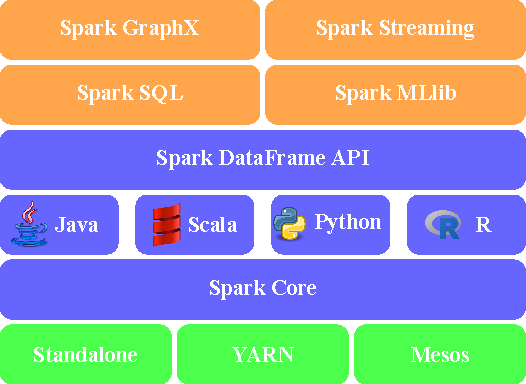
\includegraphics[width=0.6 \linewidth]{figures/spark.pdf} \\
\caption{Spark体系架构}{Spark architecture}
\label{fig:sparkarchitecture}
\end{figure}

(1)Spark SQL

Spark SQL是Spark $1.0.0$ 版本中新加入的组件,是Spark生态系统中最活跃的组件之一,为结构化数据提供了方便的存储和查询
操作\cite{Guller2015Spark}。Spark SQL提供了方便的调用接口,用户可以通过使用Scala、Java、Python等开发基于Spark SQL API的数据处理
程序,也支持传统的SQL语句与Spark进行交互。

(2)Spark MLlib

Spark MLlib(Spark Machine Learning library)常用的机器学习算法的实现\cite{MllibMLlib}。
Spark MLlib的在机器学习方面优点主要有以下三点:\circled{1}Spark是内存计算的计算框架,这一点非常适
合机器学习算法迭代计算的特点,避免Hadoop MapReduce这类IO频繁的计算框架;\circled{2}Spark MLlib使
用和部署非常方便,支持Scala和Python交互式开发环境,方便机器学习算法使用人员快速验证算法原型系统;\circled{3}Spark MLlib作
为Spark生态系统的子成员,可以去Spark生态系统进行无缝结合。

(3)Spark GraphX

是Spark分布式图计算框架,它是常用图算法在Spark上的并行实现,并且提供了图计算中用于图和图计算中的API。
是Graph Lab和Pregel在Spark上的重写及优化,是Spark生态圈中非常重要的组件\cite{Xin2013GraphX}。

Spark GraphX的核心抽象概念是弹性分布式属性图(Resilient Distributed Property Graph),是一种点和边都带有属
性的有向多重图。它扩展了Spark RDD的抽象,实现了统一表示。弹性分布式属性图有Table和Graph两种视图,对应的这两种
视图只需要一份物理存储,两种视图都有各自的操作符,基于Spark的RDD可以很轻松的进行操作。通过分布式计算提高了效率。

(4)Spark Streaming

Spark Streaming是建立在Spark上流应用计算框架\cite{Guller2015Sparks},它将流式计算分解成一系列短小的批处理作业,也就是将输入数据
按一定大小划分为一段段的数据(Discretized Stream),每一段数据都RDD,然后将Spark Streaming中
对DStream的Transformation操作变为针对RDD的Transformation操作,将RDD经过操作变成中间结果保存在内存中。
\subsection{RDD介绍}
弹性分布式数据集RDD,是Spark的核心抽象,是对分布式内存的抽象表达,它表示已被分区、只读的、并提供了一组丰富的操作方式
来操作这些数据集合。这些数据集可以全部或者部分缓存在内存中,在多次计算间重复使用,省去了大量的磁盘IO操作。

现有的并行计算框架的数据结构在处理两种应用场景显得不够高效:\circled{1}迭代式计算,主要为分布在图计算领域和机器学习问题中;\circled{2}
交互式计算工具,操作能够立即返回结果。RDD通过高度受限的共享内存方式解决上述问题,
基于稳定物理内存中的数据集合执行批量操作(如Map,Join和Group by)
操作。与其他分布式共享内存系统选择检查点(Check Points)和回滚(Roll Back)机制不同,RDD选择血统(Lineage)机制来保证可靠的容错性,
每一个RDD记录如何从RDD中衍生出来的,一旦某个RDD发生数据丢失,根据这些记录进行重新构建,而不需要进行高昂代价的检查点操作来进行数据恢复。
虽然RDD不是通用的共享内存的抽象,却包含了高可靠性、强可伸缩性和良好的表述的能力,因此成为了Spark一切操作的核心。

RDD从本质上来讲,就是只读的集合,不过集合是分布在不同的分区上的,每个分区就是一个Dataset。RDD在进行转换的过程中产生了依赖,
如果RDD的每个分区被一个子RDD继承,那么称之为窄依赖(Narrow Dependency);若RDD的分区被多个子RDD继承,那么称之为宽依赖(Wide Dependency)。
不同的操作产生不同的依赖。图\ref{fig:dependency}分别展示了map产生的窄依赖和join产生的宽依赖\cite{Zaharia2012Resilient}。
\begin{figure}
\centering
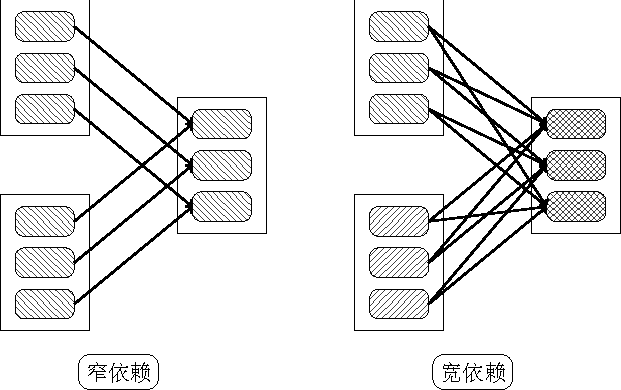
\includegraphics[width=0.6 \linewidth]{figures/rdd.pdf} \\
\caption{窄依赖和宽依赖}{Narrow dependency and wide dependency}
\label{fig:dependency}
\end{figure}

RDD提供了丰富的编程接口来操作数据集合,主要分为两种:Transformation和Action。

Transformations返回值还是一个RDD,如Map,Filter,Union等操作。它可以理解为任务分配的过程,其采用的是Lazy策略,如果是
只提交Transformation是不会提交任务执行,只有在Action操作的时候才回被触发。

Action操作是将RDD持久化起来,每调用Action操作,都会触发一次Spark的作业提交,将规划的任务(Job)提交给计算引擎,由计算
引擎将其分为多个Task,再分发相应的计算节点,开始真正处理过程。从目前的Spark的API来看,Action操作主要分为两种:\circled{1}Action操作
将标量或者集合返回给Spark的客户端程序。\circled{2}Action操作将RDD直接保存到外部文件系统或者数据库中。
\subsection{Spark优势}
Spark一栈式解决方案有很多优势,具体如下:

(1)快速处理。由于Spark采用内存计算,避免了Hadoop的磁盘操作,节省了I/O操作,在迭代式计算上Spark有着明显的优势。

(2)通用性强。Spark提供了一个强大的技术堆栈,是一个可以处理流式处理、机器学习、即时查询、图分析等多种无缝大数据处理链接计算平台。

(3)可以与Hadoop集群集成。Spark可以单独运行,也可以运行在Mesos、Yarn等集群资源管理系统上,也可以读取已有的任何HDFS数据。
\section{空间数据挖掘}{Spatial Data Mining}
空间数据挖掘是多门学科交叉研究领域,包含了多种研究技术,常用的方法有但不仅限于地理信息系统、计算几何、模式识别、机器学习、深度学习等。因此
空间数据挖掘技术丰富多彩,下面简单介绍几种常用的方法。

(1)统计分析方法 

统计方法是空间数据分析最基础的方法,以数学统计知识为基础。关注点是空间对象的非空间属性,简单的统计方法有最大值,最小值,平均值,方差等等,
复杂的方法有方差分析,P值估计等等,通常来讲这些统计结果都用图表进行表达。

(2)聚类分析方法

聚类分析方法是非监督数据挖掘中最主要的方法,通过对空间对象相似性判断,将整个空间对象划分为若干簇\cite{杨春成2004空间数据挖掘中聚类分析算法的研究}。
在聚类算法中,距离函数非常重要,常见的距离函数选择有欧几里得距离、曼哈顿距离和更通用的$L_p$距离,除了数值型属性之外,空间聚类还需要将空间位置纳入
考虑范畴,因此不同属性的应当赋予不同的权重。

(3)空间分析方法

空间分析是空间数据挖掘的特色,通过各种空间分析,对空间信息进行加工,从而发现更多知识。常见的方法有空间缓冲区分析、空间
核密度分析和空间趋势面分析等等,空间分析常常结合地学第一定律进行统计分析,拓展了统计分析方法关注的内容,发现新的知识\cite{李小文2007地理学第一定律与时空邻近度的提出}。

(4)空间关联规则挖掘方法

关联规则挖掘是根据销售事务数据库交易项商品同时出现的规律\cite{曾玲2005关联规则在空间数据挖掘中的研究},Apriori算法是关联规则挖掘最著名的
算法。空间关联规则是关联规则在空间方面的拓展,将空间关系纳入到考虑范畴。以空间关联为基础,发展出空间同位模式挖掘,比如生物在生态环境
中的共生现象。

\section{新浪微博数据接口}{Weibo API}
目前新浪微博数据获取方式主要有两种:\cite{廉捷2011新浪微博数据挖掘方案}:\circled{1}通过网络爬虫程序获取数据;
\circled{2}通过新浪微博提供了API接口获取相应主题的数据。

网络爬虫是能够自动获取并下载网页的计算机应用程序\cite{Nemeslaki2011Web},根据一定
规则不停的向网络服务器发送请求,获取特定的信息。由于互联网是通过URL进行连接,可以不间断
对整个网络内容进行获取,需要制定相应的爬虫策略,一般有与深度优先和广度优先两种调度策略。
互联网服务器则将网页中的文本内容、图片、音频视频等内容发送给应用程序,应用程序则将这些
数据按照特定的格式保存下来。

由于个人用户频繁使用爬虫从网站中获取数据将会对网站服务器带来较大的负载,因此新浪微博之类的网站会从
爬虫程序的IP地址或者验证码方式限制请求次数。而且通过爬虫获取的数据噪声较大,需要进行大量的清洗工作,
因此本文将使用新浪微博API接口获取海量空间数据。
\subsection{微博API使用}
作为丰富数据资源的平台,新浪微博给其他应用程序开放了访问这些数据的API,应用程序通过这些API获取微博内容、用户个人信息、
签到和空间位置等相关信息。这些API其实就是一系列HTTP Get请求,API接口的参数作为请求的参数发送给新浪微博服务器,
新浪微博返回相应的结果。新浪微博将这些API封装到不同编程语言的SDK中,包括了Python、Java,C\#、PHP等。

微博API的使用需要对用户的身份进行鉴别,目前新浪微博对开放平台用户采用OAuth$2.0$的方式进行授权\cite{Recordon2011The}。
OAuth$2.0$授权验证具有简单、安全等特点,是社交网络平台对外开放权限的主要方式,使用流程见图\ref{fig:api}。
\begin{figure}
  \centering
  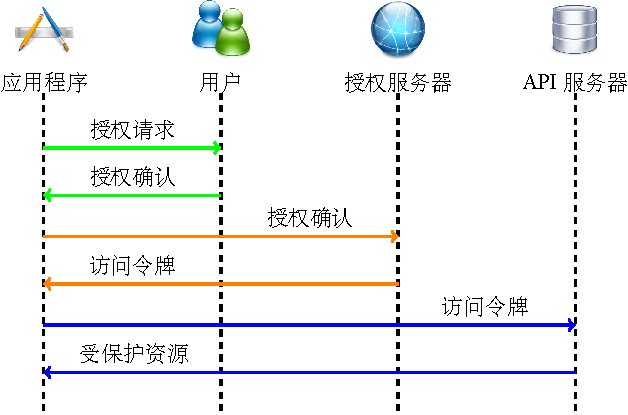
\includegraphics[width=0.6 \linewidth]{figures/api.pdf}
  \caption{新浪微博API使用流程}{The usage of weibo's api}
  \label{fig:api}
\end{figure}

第三方应用程序想要获得API接口的使用权,首先要在新浪微博开发平台进行申请应用程序的AppKey和AppSecret,
这个AppKey和AppSecret是该应用程序的标识码。用户在使用该应用程序的时候,首先要在授权页面登录自己
新浪微博账号,给予授权。然后应用程序将该用户的授权发送给新浪微博的授权服务器,返回访问令牌(Access Token)。
那么该应用可以以访问令牌访问这些API接口,获得相应的数据,在整个获取数据过程中用户的隐私得到保护。


\subsection{空间数据相关API}
新浪微博API接口主要有粉丝服务接口、微博接口、收藏接口、公共服务接口、位置服务接口、
地理信息系统接口和地图引擎接口等,部分空间数据相关API接口说明见下表\ref{tab:weiboapi}。
 \begin{table}
  \centering
  \caption{微博接口描述(部分)}{Description of Weibo api(partly)}
  \label{tab:weiboapi}
  \tabulinesep=1.5mm
  \begin{tabu}to 0.90\linewidth{X[1.1,l, m]X[1.2,l,m]}
    \tabucline[0.1em]-
    \rowfont[c]{} 接口API地址 & 说明 \\
    \tabucline-
    location/geo/address\_to\_geo & 根据地址返回地理信息坐标 \\
    location/pois/search/by\_area & 根据区域按坐标点获取POI点的信息 \\
    location/pois/show\_batch & 批量获取POI点的信息 \\
    location/citycode & 城市代码对应表 \\
    place/nearby/pois & 获取附近的POI点 \\
    place/pois/show & 获取地点的详细信息 \\
    \tabucline[0.1em]-
   \end{tabu}
\end{table}

新浪微博API接口使用非常简单,传入相应的接口指定的参数,即可返回查询结果。
以location/geo/address\_to\_geo接口为例,参数见表\ref{tab:apiparameters}。
\begin{table}
  \centering
  \caption{接口参数说明}{Description of api's parameters}
  \label{tab:apiparameters}
  \tabulinesep=1.5mm
  \begin{tabu}to 0.75\linewidth{X[1,c]X[1,c]X[2.4,l]}
    \tabucline[0.1em]-
    \rowfont[c]{} 参数 & 类型 & 说明 \\
    \tabucline-
    access\_token & String & 采用OAuth授权方式必填参数 \\
    address & String & 需要获取的坐标的实际参数 \\
    \tabucline[0.1em]-
   \end{tabu}
\end{table}

当应用程序通过该接口将符合要求的参数传入发送请求后,服务器将结果以JSON的格式将
结果返回至客户端。

\section{本章小结}{Chapter Summary}
本章首先介绍了Hadoop大数据计算框架,分别介绍了Hadoop分布式存储机制HDFS和
分布式计算模型MapReduce,并分析了其中的优缺点;然后介绍了目前流行的并行
计算框架Spark,着重介绍了Spark的核心数据结构RDD和上层应用接口;接着介绍了
常用的空间数据挖掘算法,最后介绍了新浪微博API使用方法和与空间相关数据获取接口。
\chapter{Spatial-Spark计算框架}{Spatial-Spark Computation Framework}
\section{空间数据分析处理}{Procession of Spatial Data}
\subsection{空间数据格式}
空间数据量大且空间数据格式也是各式各样。开放地理空间信息联盟(Open GIS 
Consortium, OGC)定义了一些空间矢量数据格式\cite{Bychowski2003Open},方便能够进行空间数据分析
处理和交换,下面介绍几种常用的空间矢量数据格式。

(1)WKT数据格式

WKT(Well-Know-Text)数据格式以文本形式描述,用来表示点,线和面空间对象,见表\ref{tab:wktdata}。
\begin{table}
    \centering
    \caption{WKT矢量空间数据}{Vector spatial data in WKT}
    \label{tab:wktdata}
    \tabulinesep=1.5mm
    \begin{tabu}to 0.8\linewidth{X[1.1,c]X[2.5,c]}
        \tabucline[0.10em]-
        \rowfont[c]{} 几何类型 & WKT表示方式 \\
        \tabucline-
        ST\_Point & POINT(10.05 10.28) \\
        ST\_LineString & LINESTRING (10.05 10.28 , 20.95 20.89) \\
        ST\_Polygon & POLYGON((10 10, 10 20, 20 20, 20 15, 10 10)) \\
        \tabucline[0.10em]-
    \end{tabu}
\end{table}

(2)GeoJSON数据格式

GeoJSON数据是通过JSON数据表达简单的数据格式,如点、线、多边形和这些几何类型的集合以及他们非空间属性信息,表达方式如下:
\begin{lstlisting}[
  morekeywords={type,geometry,coordinate,fields}
]
{
  "type":"feature",
    "geometry":{
      "type":"LineString",
        "coordinate":[[[-100.50,57.14],[-89.45,62.17],[-37.21,79.73]]],
        "fields":{
            "prop1":"value","prop2":"string"
            }                
    }
}
\end{lstlisting}

由于JSON格式在序列化和网络传输中的优势,非常适合分布式的数据存储,空间数据和属性数据都存储在普通的文本中。

(3)GML数据格式  

GML(Geography Markup Language)是以XML格式的空间数据表达形式,并使用XML Schema文件
定义技术,目前版本为$2.1.1$。XML Schema具有类型继承、命名空间等特性,通过XLink来表现地理空间实体的关系。
\begin{lstlisting}[language=XML]
<PhotoCollection xmlns="http://www.myhotos.org"
    xmlns:gml="http://www.opengis.net/gml"
    xmlns:xsi="http://www.w3.org/2001/XMLSchema-instance"
    xsi:schemaLocation="http://www.myphotos.org" >
    <items>
      <item>
        <name>Lynn</name>
          <description>A shot of the falls</description>
          <where>North Vancouver</where>
          <position>
            <gml:Point srsDimension="2" 
              srsName="http://www.opengis.net/def/crs/EPSG/0/4326" >
                <gml:pos>49.40 -123.26</gml:pos>
            </gml:Point>
          </position>
      </item>
    </items>
</PhotoCollection>
\end{lstlisting}

\subsection{空间数据转换}
空间数据来源各异,每种数据来源有各自的坐标参考系统,如GPS接收机获取的地理空间数据
是以WGS$84$坐标系统为基准;摄影测量往往采用该区域最适宜的坐标参考系统为基准。不同的
大地坐标系统和平面投影系统往往使得空间数据处理和分析正确性得不到保证,因此很有必要
将多源空间数据纳入到同一个空间参考系统下。

Proj.$4$是开源GIS中著名的地图投影库\cite{Urbanek2012proj4},在GRASS GIS, MapServer, PostGIS等众多GIS
软件中都直接或者间接使用Proj.$4$,$2008$年OSGeo将Proj.$4$纳入到MetaCRS的一部分,Proj.$4$
的主要功能是提供了大地坐标系和投影坐标之间的正反算,不同参考基准的坐标变换。Proj.$4$使
用C语言编写,但不同的语言也有各自相应的Proj.$4$库,如Java语言的Proj$4$j,C\#语言的Proj$4$.Net,JavaScript语言
的Proj$4$js等等。

以Java语言的Proj$4$j库为例,Proj$4$j 主要模块的如下:

(1)Datum基准

定义了空间椭球基准,主要参数包括椭球的名称,长半轴和短半轴,以及质心偏离中心的位置,Proj4j
内置了若干个常用的椭球基准如WGS84,IRE65等。

(2)CoordinateReferenceSystem参考系统

不同的坐标参照系统需要指定不同的参数,如高斯投影的坐标参考系统需要指定中央经度和投影带宽度,而
兰伯特投影需要指定投影的第一纬度、第二纬度,中央纬度和中央经度。

(3)Projection投影

Proj4j提供了$96$种投影方式,Projection是这些投影类的基类,每个投影类提供了project函数和projectInverse
函数,分别代表了投影正算和投影反算。

(4)CoordinationTransform坐标换算

坐标转换提供了不同坐标参考系统之间坐标换算类,如将高斯投影坐标换算兰伯特投影坐标,通过两个坐标参考系统
对象创建坐标换算类,生成CoordinationTransform对象,调用transform函数完成坐标换算。

\subsection{空间数据分析}
空间数据分析的正确性是GIS的一个重要参照指标,尤其在涉及空间数据数据几何拓扑关系时需要严格正确。JTS Topology Suite
是加拿大Vivid Solutions公司提供的一套开源的空间几何对象拓扑操作工具包,主要包含的功能和特色如下:

(1)实现了OGC关于简单要素的SQL查询规范定义的空间数据模型。

(2)完整的、一致的和基本的二维空间算法的实现,包含了空间分析和空间运算\cite{Johansson2002Using}。

(3)提供了常见的空间数据格式读写接口。

JTS Topology Suite在GIS中最重要的应用是计算两个几何对象之间的空间拓扑关系,每个派生自Geometry类的几何
对象都能够进行相互空间分析和空间运算,详细见表格\ref{tab:spatialanalysisoperation}。
\begin{table}
  \centering
  \caption{空间分析和空间运算}{Spatial analysises and spatial operations}
  \label{tab:spatialanalysisoperation}
  \tabulinesep=1.5mm
  \begin{tabu} to 1.0 \linewidth{X[1,c,m]X[1.4,c,m]X[2,c,m]|X[1,c,m]X[1.4,c,m]X[2,c,m]}
  \tabucline[0.1em]-
  类别 & 函数 & 功能 & 类别 & 函数 & 功能 \\
  \tabucline-
  \multirow{6}{*}{空间分析} & Contain & 包含关系 & \multirow{2}{*}{空间分析} & Overlap & 重叠关系 \\
  	& Equal & 相等关系 &  &Touch & 相接关系  \\
	\tabucline{4-6}
	& Intersect & 相交关系 & \multirow{4}{*}{空间运算} & Buffer & 缓冲区运算 \\
	& Within & 内部关系 &	& Intersection & 交集运算\\
	& Disjoint & 相离关系 & 	& Difference & 差集运算 \\
	& Cross & 内部相交关系 &  & Union & 并集运算\\
\tabucline[0.10em]-
\end{tabu}
\end{table}

\section{RDD空间扩展}{Spatial Extension of RDD}
空间数据爆炸式增长对空间数据处理提出了新的挑战,主要有以下两点:\circled{1}系统可扩展性(System Scalability):
数据的存储、读取和写入能够有效地处理GB、TB级别甚至PB级数据;\circled{2}交互式高性能(Interactive Performance):
在处理空间数据查询后,能够高效回应查询请求\cite{Yu2015GeoSpark}。

\subsection{空间数据类型}
Spark采用抽象数据类型RDD,通过分布式平行数据结构处理海量数据,使用独特的内存计算使得在处理数据
方面有着较高的性能优势。但是RDD没有完善的空间数据支持和空间操作,因此开发人员需要在Spark提供API上层重新定义空
间数据读写和操作函数,但这些没有统一的标准。

为了在分析海量空间数据时能够专注于分析算法,本文设计出一套海量空间数据分析框架:Spatial-Spark。Spatial-Spark扩展
了Spark RDD,使之能够支持常见的空间数据类型、空间索引和空间操作,整个Spatial-Spark体系结构见
图\ref{fig:spatialsparkarchitecture},底层为数据存储层,核心部分为中间Spatial-RDD空间几何对象层,最上层为
空间分析层,提供了高度定制的API接口。
\begin{figure}
  \centering  
  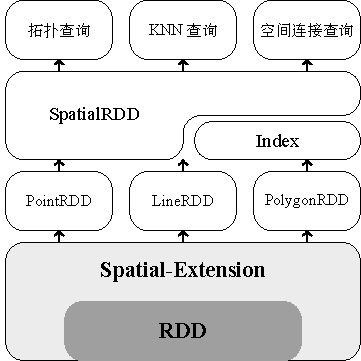
\includegraphics{figures/spatialspark.pdf}\\
  \caption{Spatial-Spark体系架构}{Spatial-Spark architecture}
  \label{fig:spatialsparkarchitecture}
\end{figure}

空间数据类型是Spatial-Spark的核心,通过RDD将点、线和面分别封装成PointRDD、LineRDD和PolygonRDD。这些Spatial-RDD表
示在集群中并行分区存储空间几何对象的集合,主要有两种方式生成Spatial-RDD:\circled{1}从HDFS中读取数据,主要流程见图\ref{fig:spatialrdd},文本空间
数据以行记录存储在HDFS中,先经过文件格式装换,将WKT,GeoJSON等数据转换成空间对象,再空间数据坐标参考系统转换统一,最
后生成Spatial-RDD,其中转换和投影步骤以接口形式提供,用户可以重写接口,完成定制化需求;\circled{2}Spatial-RDD相互之间空间运算,如PointRDD
可以通过缓冲区操作生成PolygonRDD对象,PolygonRDD对象通过提取重生成PointRDD。
\begin{figure}
\centering
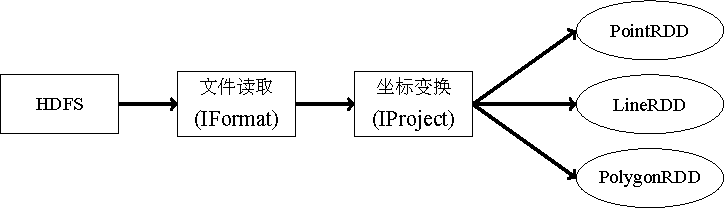
\includegraphics[scale=0.9]{figures/spatialRDD.pdf}
\caption{HDFS生成Spatial-RDD流程}{Generating Spatial RDD from HDFS} 
\label{fig:spatialrdd}
\end{figure}


\subsection{空间数据索引}
\subsubsection{RDD分区}
RDD内部数据集合在逻辑上(以及物理上)被划分为多个小集合,这样每个小集合就被成为分区。以图\ref{fig:rddpartition}为例,
RDD1有五个分区(Partition),分布在四个DataNode上面,而RDD2有三个分区,分布在
三个DataNode上面。在源码级别,RDD类存储一个Partition列表,每个Partition对象都包含
一个index成员,通过RDD编号加index就能从唯一的分区的Block编号\cite{Zaharia2012Resilient},持久化的RDD就能通过这
个Block变化从HDFS中获取对应的分区数据。
\begin{figure}
\centering
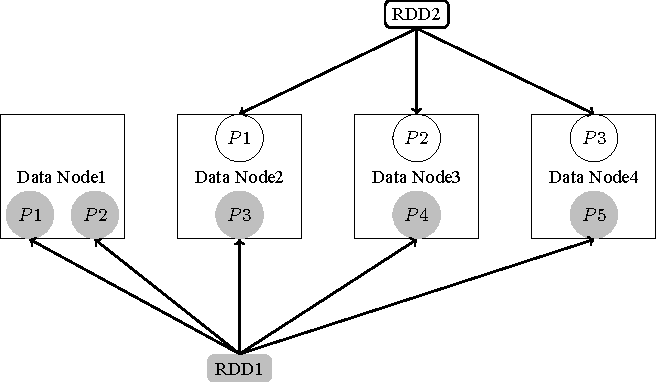
\includegraphics[scale=0.8]{figures/rddpartition.pdf}
\caption{RDD分区}{RDD partition illustration}
\label{fig:rddpartition}
\end{figure}

分区的个数决定了并行计算的粒度,多个分区能够并行计算,充分利用分布式计算资源。通常来讲,分区
的数量为计算集群的CPU核心数量的$3-4$倍。创建分区的方法主要有两种:\circled{1}在SparkContext对象读取数据
的时候指定分区的数量;\circled{2}调用RDD的分区器函数,进行重新分区。Spark在读取数据时默
认使用哈希分区器,该分区器实现简单,运算速度快,但缺点是不关心键值的分布情况,其散列到不同分区的概率会
因数据而异。往往会带来分区负载的不平衡性。

考虑到空间数据空间分布特点,Spatial-Spark提供了空间分区,重写了Partitioner函数,能够尽可能
将空间上分布相邻的空间对象处于同一RDD分区。具体算法步骤如下:

(1)根据空间要素集合的边界(boundary)和分区数量n,将整个boundary划分为$\sqrt{n}\times \sqrt{n}$个
网格,每个网格拥有一个id值。

(2)将\verb|RDD<Geometry>|进行Map或者MapPartition操作,使之转换为PairRDD<Integer,Geometry>描述
的Key-Value对象,其中Key为网格中与其相交或者包含的网格的id值,如果有多个网格与之相交,取其中一个。

(3)对\verb|PairRDD<Interger,Geometry>|按照key进行重分区计算,使每个分区能够拥有分布较为均匀的
几何对象,而且尽量保证相邻的空间的对象在同一个分区。

\subsubsection{分区索引}

好的空间索引能够极大地方便海量空间数据查询,而空间数据中最常用的空间数据索引方式就是R树。R树索引是有
美国加州大学Guttman A.教授提出的一种空间数据库的动态索引算法\cite{Guttman1984R},该数据结构的核心思想是通
过最小外包矩形(Minimum Bounding Rectangle, MBR)表达一个或者一组空间几何对象。与B树一样,R树是一棵高度平衡树,
将所有的空间几何对象都存放在叶节点,插入和删除节点不需要完全重构R树,只需要在局部进行相关拓扑调整即可,
一棵典型的R树如图\ref{fig:rtree}所示。
\begin{figure}
\centering
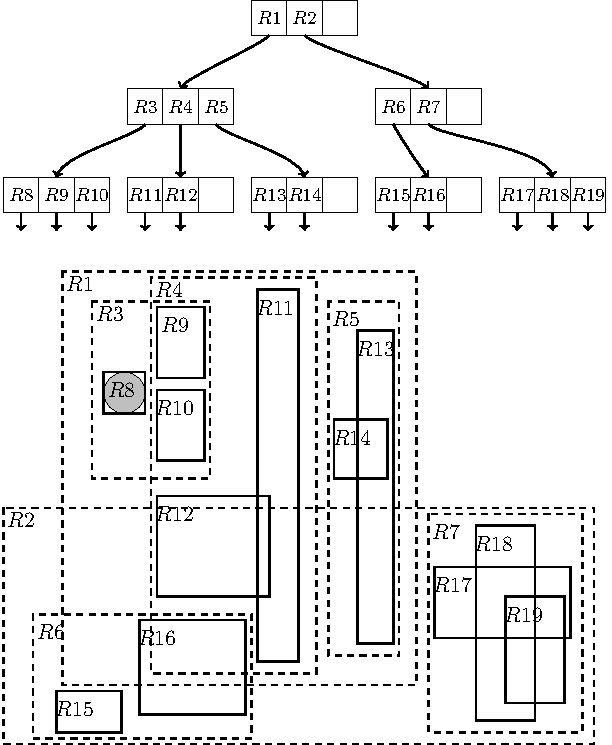
\includegraphics[scale=0.8]{figures/rtree.pdf}\\
\caption{R树示意图}{R tree illustration}
\label{fig:rtree}
\end{figure}

(1)R树插入

作为B树的一个变种,R树的插入与B树相类似,首先根据待插入空间对象的最小外包矩形待确定插入的叶节点,
然后插入对象,如果该叶节点包含的空间对象数目超过规定的最大数目,则将该节点进行分裂\cite{Huang2001Optimizing},并
将其中的一个节点向上传递,递归执行,如果直至根节点,完成树高度的提升。节点分裂的好还的标准是两个新节点的最小外包
矩形的面积之和最小。

(2)R树查询

R树查询只能检索出与给定窗口相交的空间实体对象。如果两个最小外包矩形是分离的,那么他们所代表的空间实体也肯定
是分离的,但如果两个最小矩形有相交,不能保证所包含的空间几何实体能够窗口相交。因此,R树空间检索检索策
略是:

过滤:从R树中筛选出候选节点,排除那些的不能满足相交条件的几何对象,但在候选几何对象中也
可能包含一些不满足条件的对象。由于判断最小外包矩形是否相交的计算成本低,可大幅度提高计算效率。

精选:依次判断每个候选几何对象,判断与查询窗口是否相交。可以借助JTS Topology Suite工具判断几何对象之间的拓扑关系。

在Spatial-Spark框架中,为了加快空间分析的速度,可选择在RDD的每个分区建立R树空间索引。通过RDD的MapPartition函数
将同一分区的空间对象汇集起来,每个分区建立一棵R树,将同一分区的几何对象的最小外包矩形插入树中。
通过Spark缓存机制,将索引内容缓存到Spark内存中,方便后续查询分析等工作。

\subsection{空间数据查询}

空间查询是GIS中最重要组成部分,在大规模空间数据中查询也提出了空间数据查询实时性要求。Spatial-Spark
在Spatial-RDD上层提供了空间查询层,包括空间拓扑查询(Spatial Topology Query),空间k邻居
查询(Spatial k Nearest Neighbor Query)和空间链接查询(Spatial Join Query)。使用者向
查询层发起空间查询请求,Spatial-Spark将查询的结果返回。如果空间数据在Spatial-RDD层事先建
立的了索引,那么用户可以借助索引,提高查询速度。

\subsubsection{空间拓扑查询}
空间拓扑关系是空间分析的特色,空间拓扑查询过程是给定一个空间几何对象和空间拓扑关系条件,从特定的
空间数据集筛选出符合条件的空间数据。

平面空间实体对象引入空间实体外部、内部和边界,构成了空间实体的基本组件。假设空间实体$A$的边界$\partial A$,
内部为$A^{\circ}$,补为$A^{-}$,空间实体$B$的边界为$\partial B$,内部为$B^{\circ}$,补为$B^{-}$,两两的交集就构
成了空间关系描述的9元组矩阵\cite{谢俊平2012拓扑关系和方向关系的统一表达模型}。
\[ R(A,B) = 
\begin{bmatrix}
\partial A \cap \partial B & \partial A \cap B^{\circ} & \partial A \cap B^{-} \\
A^{\circ} \cap \partial B & A^{\circ} \cap B^{\circ} & A^{\circ} \cap B^{-} \\
A^{-} \cap \partial B & A^{-} \cap B^{\circ} & A^{-} \cap B^{-} \\
\end{bmatrix}
\]

矩阵中每一个元素的取值都有空集和非空集两种,9个元素共存在512中可能,当然其中绝大部分
的空间拓扑关系时不存在的。以点、线和面为准给出所有可能空间对象之间可能拓扑关系,见表\ref{tab:geometrytopo}。
\begin{table}
  \centering
  \caption{空间几何拓扑关系}{Geometry topology rules}
  \label{tab:geometrytopo}
  \tabulinesep=1.5mm
  \begin{tabu}to 0.7\linewidth{X[1, c]X[1.2,c]X[1.2,c]X[1.2,c]}
    \tabucline[0.10em]-
    几何对象 & 点 & 线 & 面 \\
    \tabucline-
    点 & Equal\par Disjoint & Within\par Disjoint & Within\par Touch\par Disjoint \\
    \tabucline-
    线 & Contain\par Disjoint & Equals\par Within\par Overlap\par Contain\par Disjoint\par Intersect\par 
      & Within\par Disjoint\par Touch\par Intersect \\
    \tabucline-
    面 & Contain\par Disjoint & Contain\par Disjoint\par Touch\par Intersect\par &
    Equal\par Within\par Disjoint\par Touch\par Intersect\par Overlap\par Contain\par \\
    \tabucline[0.10em]-
  \end{tabu}
\end{table}

RDD中的filter算子可以筛选RDD中符合条件的元素,Spatial-Spark实现了Function接口的
通用空间拓扑查询类。该类接受待查询的空间元素Geometry和待判断的空间拓扑关系条件Condition。在
类中重写call函数即可,通用实现如下。
\begin{lstlisting}[language=Java]
@Override
public Boolean call(Geometry goe){
    return geo.condition(this.query)
}
\end{lstlisting}


当在Spatial-RDD中如果已经在每个分区构建好R树索引,可以通过索引查询相交(Intersect)、包
含(Contain)、相等(Equal)、重叠(Overlap)和被包含(Within)的拓扑关系。RDD中的FlatMapPartition算子
可以对每个分区进行操作,并将结果展平(Flat)返回,用户定义Spatial-Spark预先实现了FlatMapFunction接
口的类,该类构造函数只包含带查询对象的最小外包矩形(Envelope),通过R树高效的查询函数返回最小外包矩形与待查询
的外包矩形的空间几何对象。索引查询是初步空间查询,在返回的结果中,在对数据进行精确空间拓扑查询,通用实现如下。
\begin{lstlisting}[language=Java]
@Override
public Iterator<Geometry> call(Iterator<STRTree> t){
    STRtree tree = t.next()
    return tree.query(this.query.getEnvelopeInternal())
}
\end{lstlisting}

\subsubsection{空间k邻居查询}
空间K个近邻居查询在现实生活中有着广泛应用,尤其在移动互联网时代,位置推荐、商场选址和公共交通等方面有着
广泛应用\cite{董亭亭2013大数据下空间数据索引和}。Spatial-Spark在K邻居查询,算法借助优先级队列数据结构,
算法主要分为两步:\circled{1}选择:针对每个分区,接受一个查询点和查询邻居数量K,在该分区中,构建一个容量
为K的优先级队列,依次将计算查询点与分区内几何对象的空间欧氏距离,并添加至优先级队列中,如果队列已满,将
集合中距离最大元素删除再添加;\circled{2}合并:针对每个分区的优先级队列,再次筛选出前K个最小距离的几何
要素,KNN通用查询类如下。
\begin{lstlisting}[language=Java]
@Override
public Iterator<Geometry> call(Iterator<Geometry> inputs){
        while(inputs.hasNext()){
            if(pq.size()< this.k){
                pq.offer(inputs.next());
            }else{
                Geometry geo = inputs.next();
                double distance = geo.distance(this.query);
                double longestDistance = pq.peek().
                                    distance(this.query);
                if(longestDistance > distance){
                    pq.poll();pq.offer(geo);
                }
            }
        }
}
\end{lstlisting}


\subsubsection{空间连接查询}
空间连接查询是常用且复杂的空间数据查询操作,类似于数据库的两张表Join查询,从两个空间对象集合中查询出符合特定空间关
系的空间几何对象对\cite{Jacox2007Spatial}。例如两个空间数据集A和B,空间连接是从A中的空间对象到B中的空间对象使用空间拓扑
关系$t$,返回分别来自A和B的满足条件的几何对象对,空间对象的复杂性和海量性将会导致空间连接运算需要大量的
计算,时间复杂急剧上升。Spark的并行计算特点为空间连接运算提供了新的模式,因此Spatial-Spark采用了并
行化方式实现了空间连接查询算法。算法的主要步骤分为两步。

(1)过滤步骤

借鉴Spatial-Spark空间分区算法,首先将其中任意空间数据集的边界按其最小的几何对象外包
矩形分割成规则的网格,每个网格赋予编号。将空间数据集的每一个元素与判断与之相交的最小外包矩形
编号,通过RDD相应的MapToPair操作转换成PairRDD,其中键key为网格的编号,值value为空间几何对象,再使
用转换函数cogroup,按照key将连个要素集合并起来。
\begin{figure}
\centering
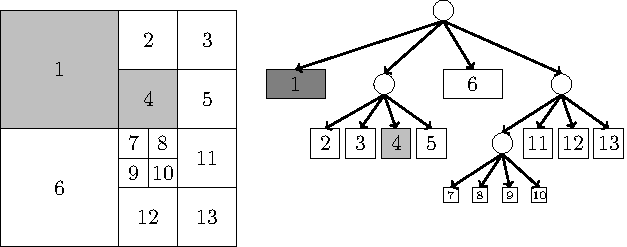
\includegraphics[scale=0.8]{figures/quadtree.pdf}
\caption{四叉树示意图}{Quadtree illustration}
\label{fig:quadtree}
\end{figure}


在空间元素最小外包矩形与格网相交时,可以预先将整个格网数据进行预处理。四叉树也是一种树状索引数据
结构,地理空间对象局部范围信息可以用四叉树进行存储,其采取从整体到局部划分的方式建立索引。建立过程
如下:对空间范围平面平均分成四个部分,如果改部分的空间对象属性一致,则不再划分,否则继续划分四个小
部分,如此重复递归执行。每划分一次,四叉树深度增加1,对于深度为$n$的四叉树索引,包含的空间对象至多为($2^n \times 2^n$)个,
四叉树示意图见\ref{fig:quadtree}。

对于空间连接查询中预先处理的格网建立的四叉树索引,所有的叶节点的深度相同,平均每次查询的时间复杂
度为$\log_{4}n$,而遍历整个格网的时间复杂度为$n$。

(2)求精步骤

在过滤阶段中,同一网格内空间对象,再根据空间拓扑要求精确筛选,返回结果中每个元素表示
一对满足条件的空间拓扑要求的几何对象对,整个空间连接过程见算法\ref{alg:join}。
\begin{algorithm}[h]   
\caption{空间连接查询}
\label{alg:join}
\begin{algorithmic}[1] %这个1 表示每一行都显示数字  
\REQUIRE  ~~\\ %算法的输入参数:Input  
空间RDD1:spatial\_rdd1;\\  
空间RDD2:spatial\_rdd2;\\  
\ENSURE ~~\\ %算法的输出:Output  
空间连接对象对, spatial\_join; \\
\STATE $//$与网格相交生成key-value;
\STATE spatial\_pair\_rdd1 = spatial\_rdd1.flatToPair(); \\ 
       spatial\_pair\_rdd2 = spatial\_rdd2.flatToPair();
\STATE $//$按key进行cogroup操作;

\STATE spatial\_pair\_groups = spatial\_pair\_rdd1.cogroup(spatial\_pair\_rdd2);

\STATE $//$每个value进行详细拓扑判断

\STATE spatial\_pair\_values = spatial\_pair\_groups.mapValue();  

\STATE $//$去重操作 
\STATE spatial\_pair\_join = spatial\_pair\_values.reduceByKey(); 
\STATE $//$去掉key 
\STATE spatial\_join = spatial\_pair\_join.mapToPair(); 
\RETURN spatial\_join; %算法的返回值  
\end{algorithmic}  
\end{algorithm} 


\section{Spatial-Spark实验分析}{Experiments and Analysises of Spatial-Spark}

\subsection{实验平台及配置}
为了验证Spatial-Spark计算框架在空间数据分析中的优势,搭建了Hadoop/Spark计
算集群\cite{Ghosh2017Install1, Ghosh2017Install2},整个集群有$10$台服务器组成,
每台服务器安装了VMware虚拟机,每台虚拟机使用的操作系统为Centos $6.4$ Linux操作
系统,每台虚拟机的配置见表\ref{tab:clusterconfig}:
\begin{table}
  \centering
  \caption{集群配置}{Cluster configurations}
  \label{tab:clusterconfig}
  \tabulinesep=1.5mm
  \begin{tabu}to 0.5\linewidth{X[1, c]X[1,c]}
    \tabucline[0.10em]-
    项目 & 配置  \\
    \tabucline-
    内存 & $4$G \\
    CPU核心 & 双核四线程 \\
    硬盘容量 & $30$G \\
    操作系统 & CentOS $64$位 \\
    Hadoop版本 & $2.6$ \\
    Spark版本 & $1.4$ \\
    JDK & $1.7$ \\
    以太网络 & $1000$Mbps \\
    \tabucline[0.10em]-
  \end{tabu}
\end{table}

Hadoop/Spark集群部署繁琐,涉及到各个方面的技术,其中包括Linux系统的配置,Hadoop的配置与
调试,Java和Scala语言库的安装,Spark计算框架配置和部署。 为了能够使集群能够相互通信,对
$10$台服务器IP地址划分和Hostname修改,因为集群之间需要进行数据交换处理,所以要配置使节点之
间能够SSH免密码通信。各节点IP配置见表\ref{tab:ipclusterconfig}:
\begin{table}
  \centering
  \caption{节点IP}{Nodes' IP addresses}
  \label{tab:ipclusterconfig}
  \tabulinesep=1.5mm
  \begin{tabu}to 0.8\linewidth{X[1,c]X[1,c]|X[1, c]X[1,c]}
    \tabucline[0.10em]-
    节点 & IP地址 & 节点 & IP地址  \\
    \tabucline-
    Master & $192.168.5.100$ & Node$5$ & $192.168.5.105$ \\
    Node$1$ & $192.168.5.101$ & Node$6$ & $192.168.5.106$ \\
    Node$2$ & $192.168.5.102$ & Node$7$ & $192.168.5.107$ \\
    Node$3$ & $192.168.5.103$ & Node$8$ & $192.168.5.108$ \\
    Node$4$ & $192.168.5.104$ & Node$9$ & $192.168.5.109$ \\
    \tabucline[0.10em]-
  \end{tabu}
\end{table}

其中Master节点为主节点,守护Hadoop的Namenode进程、Yarn的ResourceManager进程和Spark的
Master进程。而Node$1\sim $Node$9$节点为从节点,守护Hadoop的Datanode进程和Spark的Worker进程,其
中Node1节点另外守护Hadoop SecondaryNameNode进程,当Master节点的Namenode进程出现
故障,Node$1$节点将被担当起NameNode节点的作用。

Spark计算模式主要分为三种:Local模式、Standalone模式和Yarn-Cluster模式。Local模式是在
本地运行,Spark的Local模式部署简单,适合单机上调试编写的Spark 应用程序;Standalone模式
是Spark自身实现资源调度框架\cite{Fern2016Automated},当不需要其他计算框架的时候如MapReduce、Storm等,只使用
Spark进行大数据计算时,可以采用Standalone模式,其中Spark Shell交互式运行环境就是运行在
该模式之上;Yarn-Cluster模式借助Yarn统一管理整个计算资源,用户在Yarn集群中的服务和Spark
应用的资源完全隔离。

为了方便调试,本实验采用Standalone模式,当整个集群配置完毕后,启动Spark-Shell,采用Scala
交互式语言编写WordCount程序,返回正确结果表明整个hadoop-spark集群配置成功。
\subsection{实验对比分析}

(1)MapReduce与Spatial-Spark空间过滤筛选对比

在相同的集群中,分别编写MapReduce应用程序和Spatial-Spark应用程序,对相同规模的空间数据进
行空间数据分析。选用的数据为全国所有道路线状空间对象(包括高速公路、国道、省道、县道),首先
对原有的ShapeFile数据转换成OGC标准的WKT文件,按行存储为一个空间对象,在集群中通过Hadoop相关命
令,存放到HDFS中,集群中HDFS的Block的大小为$128$M。空间过滤算法定义为选择其中一条道路,求解
其外包矩形中包含的所有其他道路。

实验分为五组,实验数据量分别为$200$M、$500$M、$1$G、$2$G和$3$G,结果见图\ref{fig:topycomparsion},当数据量不大的
时候,Spatial-Spark相对于MapReduce优势不够明显,当数据量达到一定程度后,Spatial-Spark内存
计算的优势突显出来,在相同的条件下,MapReduce消耗的时间是Spatial-Spark的两个数量级。
\begin{figure}
  \centering
  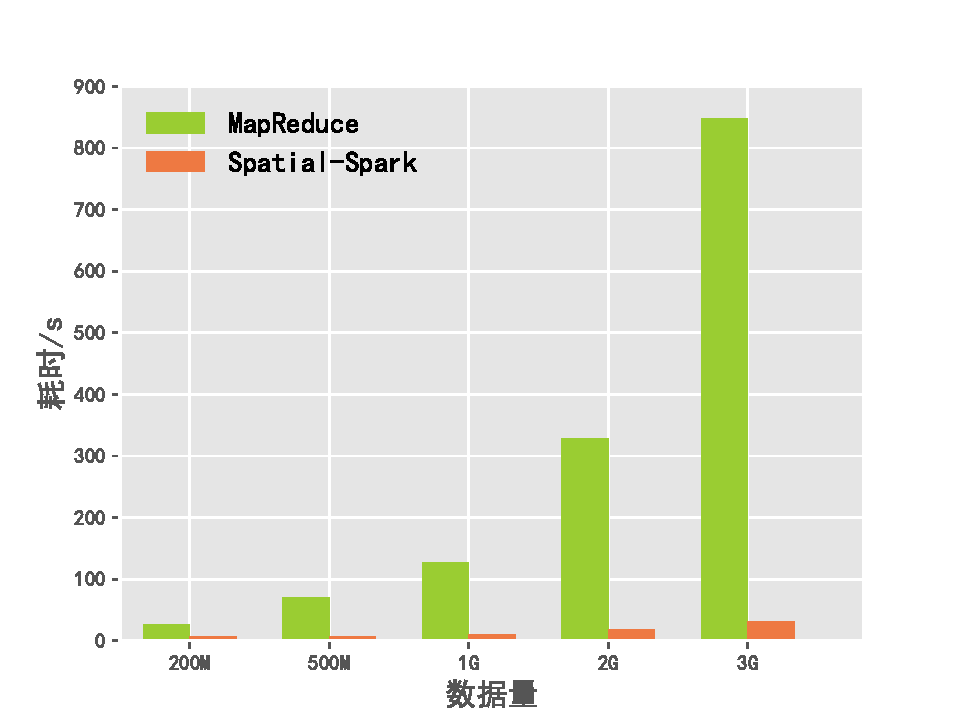
\includegraphics[scale=0.7]{figures/topo_query.pdf} \\
  \caption{MapReduce和Spatial-Spark查询对比}{MapReduce and Spatial-Spark topology query comparsion}
  \label{fig:topycomparsion}
\end{figure}

(2)Spatial-Spark集群扩展性能分析

Spatial-Spark计算框架的优越性在于其横向扩展性(Scale Out),通过增加廉价的计算机,使得
计算性能呈现显著性增加。在空间大数据分析中也不例外,本实验通过分析动态调整工作节点的
数目,比较在相同的数据规模下各个不同工作节点数目下,消耗的时间对比。

空间连接查询是空间运算中计算量较大的运算,选用的数据为全国县界面对象,共2917个面对象,与
全国道路中进行连接操作,获取每个县与之相交的道路。

实验共分为四组,使用的Work Node的数量分别为$2$、$4$、$6$和$8$,实验数据量$150$M县界对象,$1$G的全国道
路。为实验结果见图\ref{fig:node_memory},第一组实验引发java.lang.OutOfMemoryError异常,集群内存不足。其余
实验组时间消耗大致相同。

内存大小也是影响Spatial-Spark运算速度中重要因素,Spark在提交任务时候,可以通过executor-memory参数指
定每个工作节点提供给本次计算的内存,Standalone工作模式将会统一管理这些内存和资源调配。通过调整
内存参数,分析空间链接操作耗时。
\begin{figure}
  \centering
  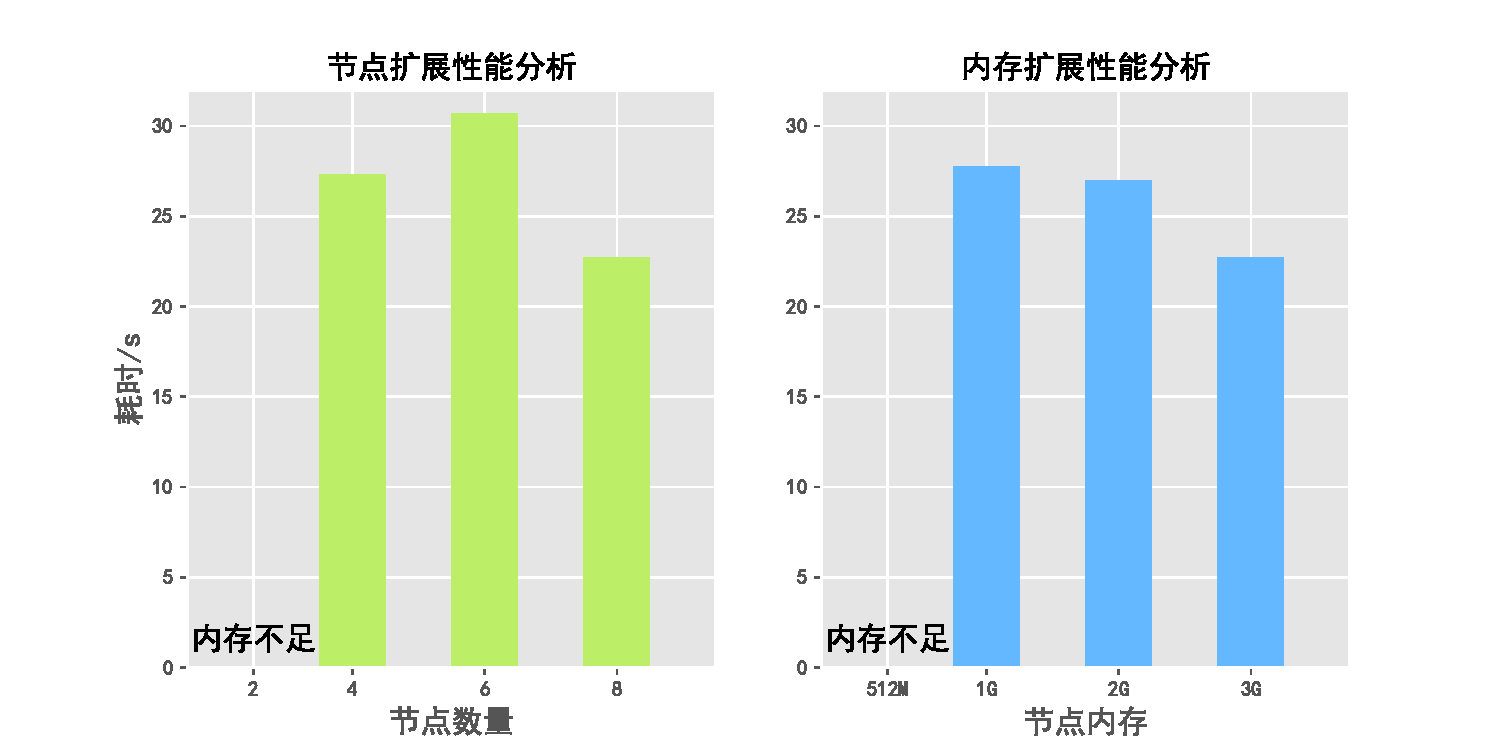
\includegraphics[scale=0.5]{figures/node_memory.pdf} \ \
  \caption{Spatial-Spark扩展性实验}{Spatial-Spark scale-out results}
  \label{fig:node_memory}
\end{figure}

实验共四组,每一组节点的内存分别为$512$M、$1$G、$2$G和$3$G,实验数据量$150$M县界对象,$1$G的全国道路。实验结
果见图\ref{fig:node_memory},第一组实验引发java.lang.OutOfMemoryError异常,集群内存不足。其余实验随着集群内存
的增大,时间消耗也呈下降趋势。

(3)Spatial-Spark空间索引性能分析

Spatial-Spark不仅仅是RDD的空间拓展,而且在分布式空间计算中引入了空间索引,并将索引通过Spark存
储策略缓存在内存中,并根据空间数据的分区,为每个分区建立了索引。由于R树索引存储的为空间对象的最
小外包矩形,因此在相关空间分析时,需要在初步筛选后进行精确空间判断分析。
\begin{figure}
  \centering
  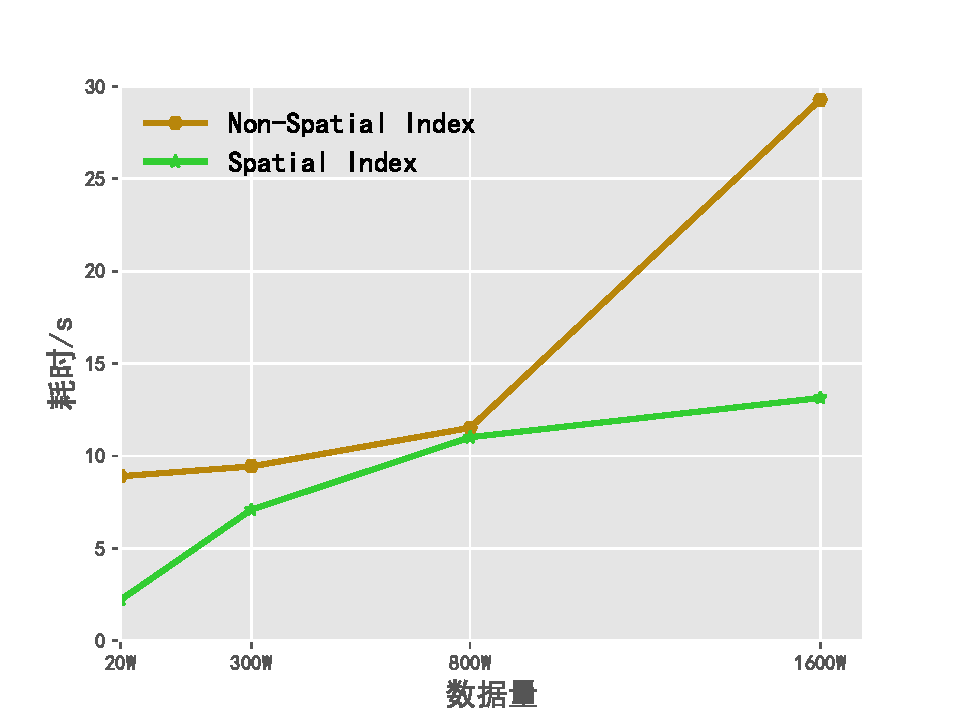
\includegraphics[scale=0.7]{figures/index.pdf} \\
  \caption{Spatial-Spark索引和非索引比较}{Spatial-Spark index Vs. non-index query comparsion}
  \label{fig:index}
\end{figure}

KNN空间查询是常用的空间数据查询分析,选择全国兴趣点(POI)共八百多万条数据,共$2.3$G,按行存储
数据,包含了空间和非空间数据。

实验总共分为四组,POI数目分别为$20$W、$300$W、$800$W和$1600$W,结果见图\ref{fig:index},对已经建立空间索引的KNN
查询消耗时间比非空间索引少,随着数据量增加,空间索引优势越发明显。
\subsection{Spatial-Spark优化方案}

Spark程序都具有「内存计算」的天性,所以集群中的所有资源:CPU、网络带宽或者内存都是成为Spark程序性能的瓶颈。

(1)数据序列化

序列化的作用是能够将数据在集群网络传输,因此序列化的对于提高分布式程序的性能起到重要的作用,一个不
好的序列化方式将会极大地降低计算速度。因此优化对象的为提高Spark应用程序的第一选择\cite{Zhao2016An}。Spark提供
了两种序列类库: \circled{1} Java序列化:在默认情况下,Spark采用Java的ObjectOutputStream序列化一个对象,只要
类实现了java.io.Serializable接口。Java序列化十分灵活方便,但是速度较慢;\circled{2}Kryo序列化:Spark也
能使用Kryo序列化对象,Kryo不仅速度快,而且生成的结果更为紧凑。但Kryo序列化使用比较繁琐,需要提
前注册要序列化的类。

在Spatial-Spark中,实验表明使用Java序列化对象某一RDD消耗为$434$M内存,当改用Kryo序列化后占该
RDD消耗$53$M内存,优化效果明显。

(2)内存优化

Spark内存计算给大数据分析带来了便利,但针对特别大的分析数据,内存无法完整加载,RDD持久化API提
供了多种序列化存储级别,见表\ref{tab:level},不同的序列化选择,使得在处理大数据时在效率和内存之间选择不同的权衡。

\begin{table}
  \centering
  \caption{存储级别策略}{Storage level stragies}
  \label{tab:level}
  \tabulinesep=1.5mm
  \begin{tabu}to 0.8\linewidth{X[1, c]X[1,c]}
    \tabucline[0.10em]-
    存储级别 & 说明  \\
    \tabucline-
    MEMORY\_ONLY & 全部序列化到内存 \\
    DISK\_ONLY & 全部序列化到磁盘 \\
    MEMORY\_AND\_DISK & 序列化到内存和磁盘 \\
    MEMORY\_ONLY\_SER & 序列化到内存字节数组 \\
    \tabucline[0.10em]-
  \end{tabu}
\end{table}

用多大内存来缓存数据是内存回收是非常重要的参数,在默认情况下,Spark采用运行内存
的$60\%$空间来进行RDD缓存,所以在程序运行期间只有$40\%$的内存可以用来创建对象。当程序运行过程中JVM频
繁进行垃圾回收,会大大减低程序运行速度,为了提高效率,可以手动修改缓存大小比例。

\section{本章小结}{Chapter Summary}

本章着重介绍了Spatial-Spark大数据空间分析框架,首先分析了矢量空间数据格式种类,空间数据转换和开源空间
数据分析包;接着对Spark核心数据结构RDD空间扩展为Spatial-RDD,并着重对空间数据进行空间分区索引,
以此为基础,构建了常见空间分析应用API。以实验为基准,分析了Spatial-Spark的性能方面的特点。

\chapter{POI空间数据分析}{Spatial Data Analysis of Weibo POIs}
新浪微博签到是新浪微博用户在使用移动终端发送微博时,使用移动终端的定位功能,
用户可以选择附近热门的位置或者自行添加位置的功能\cite{韩华瑞2016湖北省微博签到活动空间差异分析——以新浪微博为例}。
这些位置信息将会被存储到新浪微博数据服务器中,在微博网页端,可以查看该签到位置的详细信息,这些签到数据称为
感兴趣点POI(Point Of Interest)\cite{Ye2011Exploiting},见图\ref{fig:webpoi}。
\begin{figure}
  \centering
  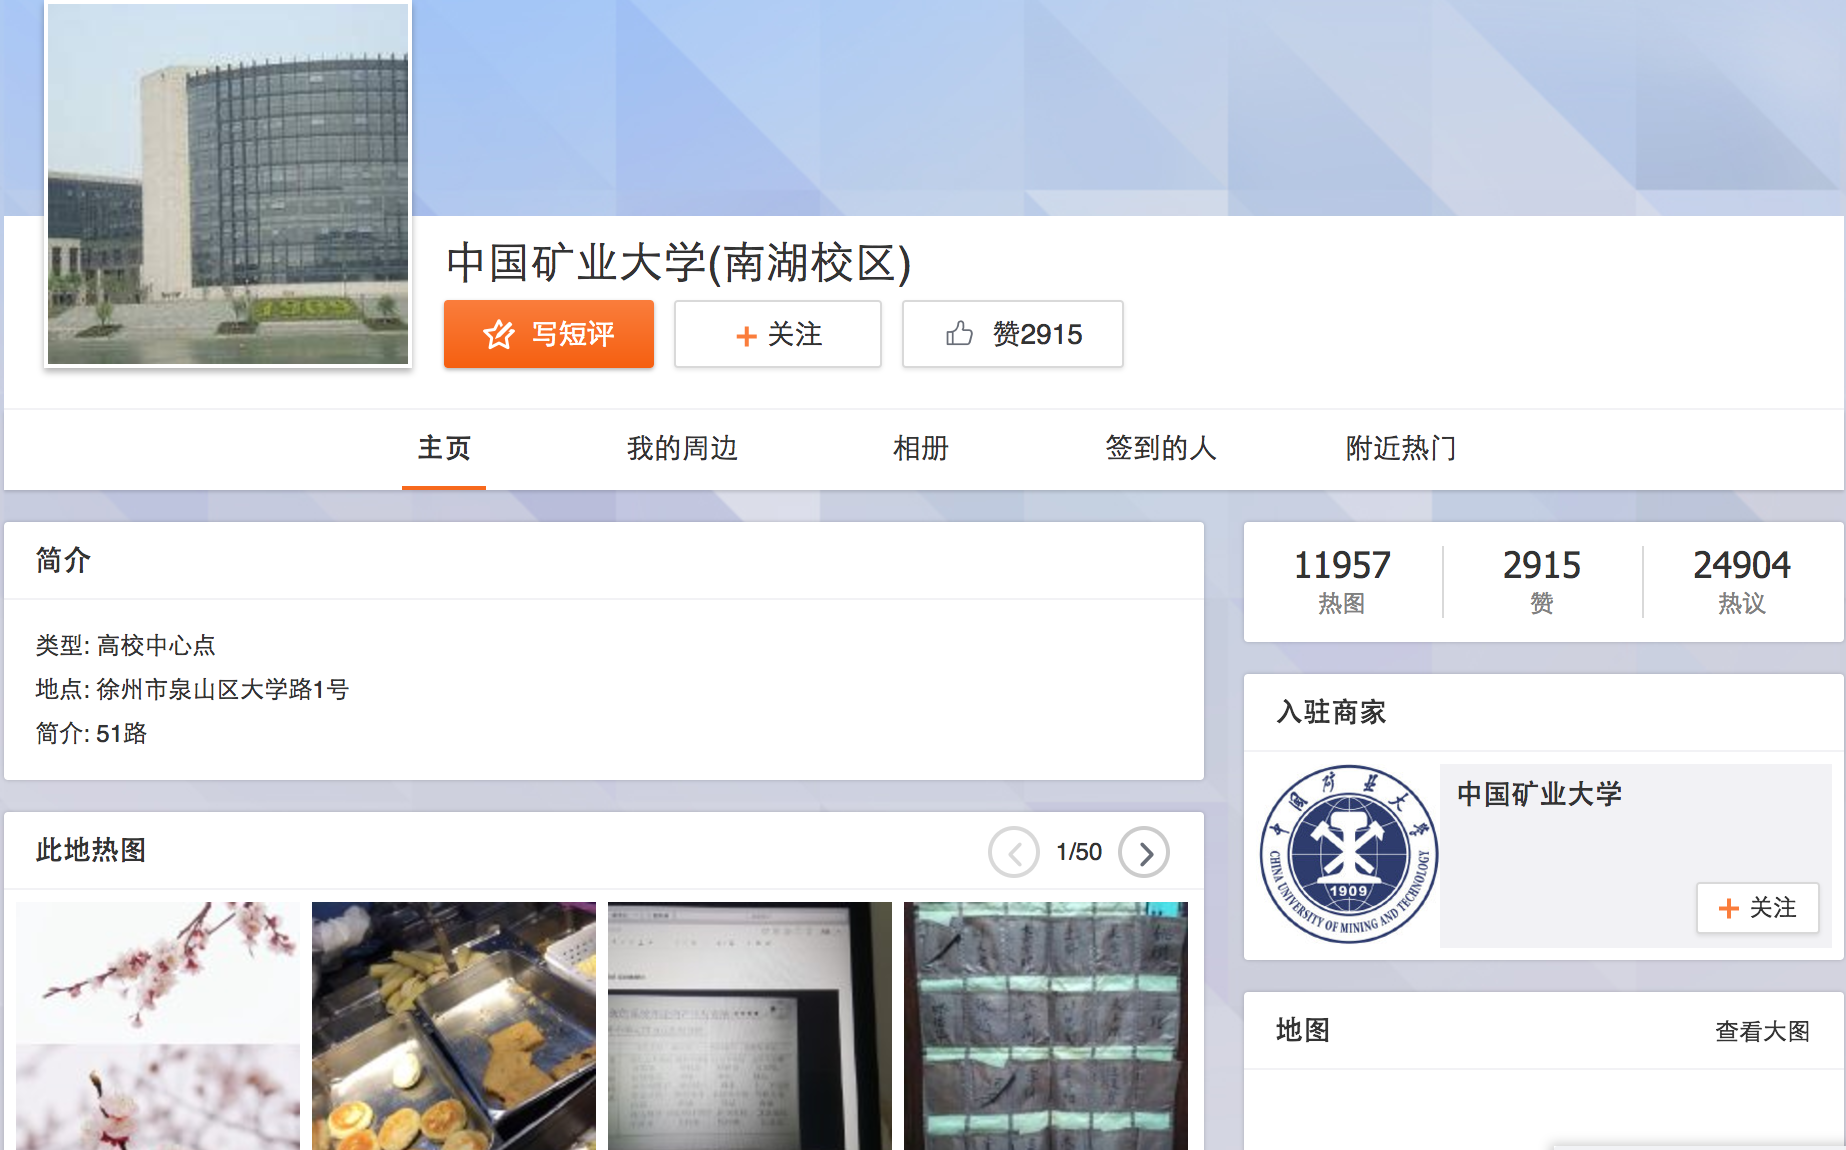
\includegraphics[width=10cm]{figures/webpoi.png} \ \
  \caption{微博网页POI}{POI in web}
  \label{fig:webpoi}
\end{figure}


\section{POI数据获取}{POI Data Fetch}

新浪微博提供了place/nearby/pois接口获取附近的POI数据,该接口参数见表\ref{tab:api_poi}。
\begin{table}
  \centering
  \caption{POI接口参数(部分)}{POI api parameters(partly)}
  \label{tab:api_poi}
  \tabulinesep=1.5mm
  \begin{tabu}to 0.8\linewidth{X[0.8,c]X[1,c]X[1,c]X[2.8,c]}
    \tabucline[0.1em]-
    接口 & 参数 & 类型 & 说明 \\
    \tabucline-
    \multirow{3}{*}{POI} & lat & Float & 纬度 \\
      & long & Float & 经度 \\
      & range & Int & 查询半径,最大10km \\
    \tabucline[0.1em]-
   \end{tabu}
\end{table}

为了获取全国范围内POI数据,需要对全国区域内进行「地毯」式查询,而上述新浪微博
API接口的坐标参考系统是不一致的,查询点经纬度属于椭球坐标系统(大地坐标系统),
而查询半径属于平面坐标系统(投影坐标系统),因此需要针对查询坐标进行一步预处理。

(1)投影:
地图投影多种多样,按照某种特定的要求地图投影可分为等角投影、等距投影和等积投影\cite{Yang1999Map},
我国常用的投影是高斯投影,但高斯投影存在离中央经线越远,变性越大等缺点,而且需要划分较多的投影带,
处理较为繁琐。
	
Lambert投影属于等角圆锥投影,通过投影圆锥面割于椭球体面的两纬线,减少南北方向的变形。Lambert
投影主要用于南北方向跨度较大的地区成图,我国绝大多数省(区)位于中纬地区,因此采用Lambert
正轴等角割圆锥投影,参数为中央经度为$105^{\circ}\text{\textrm{E}}$,第一标准纬度$25^{\circ}\text{\textrm{N}}$,
第二标准纬度为$47^{\circ}\text{\textrm{N}}$

(2)栅格化:
为了实现「地毯」式搜索,需要将投影后的全国边界面要素进行栅格化处理,
由于新浪微博API在查询半径上限为$10\text{\textrm{km}}$,为了减少查询次数,
设计方案如图\ref{fig:grid},栅格化的大小为$10/\sqrt{2} \times 2 =10\sqrt{2}=14.1\text{\textrm{km}}$
\begin{figure}
\centering
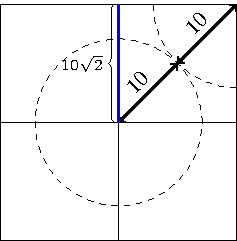
\includegraphics[scale=0.8]{figures/query.pdf}

\caption{查询示意图}{Query illustration}
\label{fig:grid}
\end{figure}

(3)投影坐标反算:
栅格化后,每个点坐标为投影平面坐标系,为了与新浪微博API接口匹配,需要将查询点的平面
坐标通过Lambert投影反算,转换成经度和纬度(椭球坐标)。

本文使用新浪微博C\# SDK开发了新浪微博数据获取应用程序,启动程序后,登录新浪微博账号,
程序向新浪微博授权服务器获取授权后,获得调用新浪微博API的权限。
为了防止频繁访问服务器而导致返回不全数据或者空数据,需要在每次完成请求后线程暂停数毫秒,同时为了
能够多进程并发执行,将查询点拆分为若干个文件,程序界面见图\ref{fig:crawler},每个进程使用一份查询点文件。
\begin{figure}
  \centering
  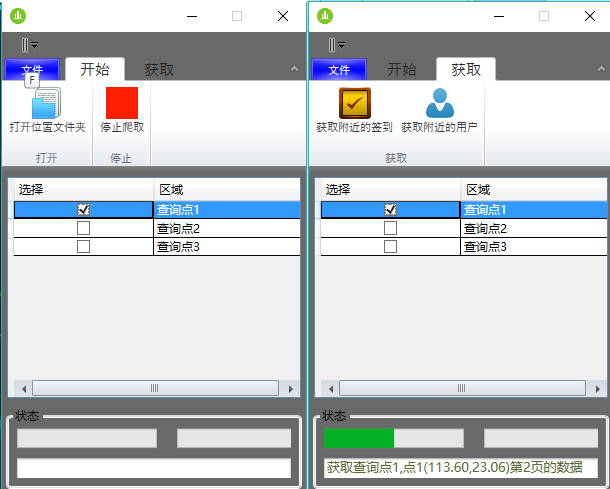
\includegraphics[width=8cm]{figures/crawler.png} \ \
  \caption{程序界面}{Program interface}
  \label{fig:crawler}
\end{figure}

这些POI包含了位置、类别、签到数目等数据,见表\ref{tab:propertiesofpoi}。
\begin{table}
  \centering
  \caption{新浪微博POI数据(部分)}{Properties of Weibo POI(partly)}
  \label{tab:propertiesofpoi}
  \tabulinesep=1.5mm
  \begin{tabu}to 0.9\linewidth{X[1,c]X[1,c]|X[1,c]X[1,c]}
    \tabucline[0.1em]-
    属性 & 说明 & 属性 & 说明 \\
    \tabucline-
    PID & POI编号 &  Name & POI名称  \\
    Longitude & POI经度 & Latitude & POI纬度 \\
    Category & POI类别 & CheckNumber & POI签到数量  \\
    \tabucline[0.1em]-
   \end{tabu}
\end{table}

新浪微博返回的数据为JSON格式,表\ref{tab:propertiesofpoi}中的每个属性值都是以key$-$value形式
保存在JSON文本中,但是由于网络或者新浪服务器等问题,有些JSON记录数据不全,噪声较多,因此这些数据不适宜保存
在传统的关系型数据库中,因为数据库表的结构需要在使用前定义,因此将获取的$900$多万条微博POI,共$2.3$G
数据按行存储到HDFS中。

\section{统计分析}{Statistical Analysis}
Spatial-Spark不仅仅支持空间数据,对于非空间数据处理仍然保留了Spark计算框架的接口,Spark RDD提供了丰富
的操作如合并(Union),去重(Distinct),过滤(Filter)等操作,方便开发者使用。

\subsection{热门签到地点}
每个POI数据都包含了签到数量,在RDD中使用sortBy和take操作,通过简单的排序,可以获取签到数
量前10位的POI,详细内容见表\ref{tab:top10poi}。
\begin{table}
  \centering
   \caption{热门签到地点}{Hottest POIs in top 10}
   \label{tab:top10poi}
  \tabulinesep=1.5mm
  \begin{tabu}to 1.0\linewidth{X[1.7,c]X[1.5,c]|X[1.7,c]X[1.5,c]}
    \tabucline[0.1em]-
    POI名称 & 签到数量 & POI名称 &  签到数量 \\
    \tabucline-
    星光公益站  & $399622$ & 丽江古城  & $160032$ \\
    浦东机场  & $184263$ & 成都双流国际机场 & $158121$ \\
    厦门高崎国际机场  & $181911$ & 望京  & $148109$ \\
    中关村 & $166640$ & 首都机场T$3$航站楼  & $140470$ \\
    深圳宝安国际机场& $162857$ & 广州白云机场 & $136998$ \\
    \tabucline[0.1em]-
   \end{tabu}
\end{table}

\subsection{热门签到类别}
每个POI数据也包含了该POI所属的类别,使用RDD的groupBy和reduceByKey两个算子,统计出每个POI类别
的数量,以新浪微博Logo制作出POI类别词云,见图\ref{fig:poiwordclound},词条频数越大,词条字体越大。
从图中可以看出生活娱乐类别是新浪微博POI类别中数量最多的,从侧面说明了新浪微博POI对人活动信息的反映,
而这些信息对商家的广告投放、微博旅游推荐\cite{朱晨曦2016基于微博签到的地理空间信息研究}有重要的参考意义。
\begin{figure}
  \centering
  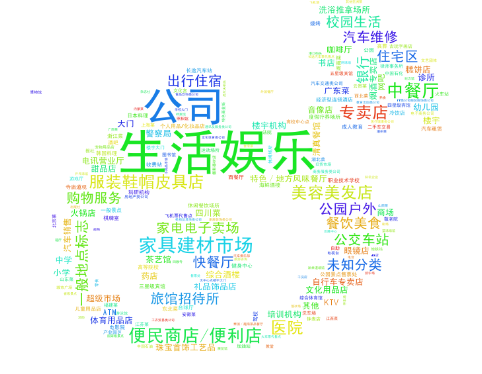
\includegraphics[width=7cm,height=5.25cm]{figures/poi_category.png} \ \
  \caption{POI类别词云}{Word cloud of pois' category}
  \label{fig:poiwordclound}
\end{figure}

\section{同位模式}{Co-Location Pattern}
频繁模式是频繁出现在数据集中的模式\cite{Agrawal1995Mining},一般认为频繁模式中的项与项之间存在
一定的相关性,同时它们之间也存在推导规则,根据一定算法可以发现事物之间关系并进行预测\cite{Agrawal1999Automatic}。
目前空间关联分析可以划分为单主题和多主题的两种模式,单主题空间模式发现是传统关联分析在空间维度上拓展,
但是存在人工干预等缺点;多主题模式单纯地寻找在空间聚集一起的事物,也就是空间空位模式(co-location pattern)。

\subsection{关联规则算法}
关联规则是无监督机器学习领域中研究最活跃、最广泛的一种算法\cite{王佐成2006空间关联规则的双向挖掘},通过对数据库
记录进行多次扫描,就可以获得非常简单的表述形式。而且关联规则也非常容易解释,数学模型描述如下:

假设事务项(Transaction)为$T$,每个事务项$T$都是由集合$I={I_1,I_2,\ldots,I_m}$组合而成,其中集合$I$中项(Item)各不相同。
$P$为项$I_i$的一个组合,如果$P$属于$T$,
则称事务$T$包含$P$,那么关联规则的表达形式是$P \rightarrow Q$,其中$P\in T, Q\in T$并且$P \cap Q=\emptyset$。
关联$P \rightarrow Q$在数据集$D$中成立,需要满足支持度$s$和置信度$c$的
约束\cite{陈江平2004空间关联规则挖掘算法研究}。置信度是事务集$D$中包含组合$P$又包含组合$Q$的百分比;支持度是
组合$P$出现的事务中,包含组合$Q$事务的百分比\cite{蔡伟杰2001关联规则挖掘综述}。

在这里定义强规则是指既要不小于支持度阈值($min\_s$)又不小于置信度阈值$min\_c$的规则,如果 
$s(P\rightarrow Q) \ge min\_s$,则称$P\cap Q$是频繁项集;如果$c(P\rightarrow Q) \ge min\_c$,则称
规则$P\rightarrow Q$成立。

关联规则挖掘算法中最著名要属Agrawal R.和Srikant R.在提出的布尔规则关联频繁集合算法(Apriori算法)
\cite{Koperski1995Discovery},该算法的核心思想为两条:\circled{1}频繁项的子集必须也是
频繁的;\circled{2}非频繁项的超集必定非频繁。因此Apriori算法主要分为两个步骤:

(1)连接步

$L_{k-1}$自相连产生$k$项集的生成$C_k$,再通过$C_k$筛选出$L_k$。根据Apriori算法第二个条件,
在生成$L_k$集合过程中,可以避免一些非频繁项连接。

(2)剪枝步

如果所有的频繁$k$项集都包含在$C_k$中,但$C_k$中的成员却不一定全是频繁的。通过Apriori算法的
第一个条件,如果某$k$项集中存在非频繁项,那么该$k+1$项必定非频繁,可将其删除做剪枝处理。

\subsection{单主题空间关联规则}
Koperski K.将传统的关联规则挖掘拓展至空间关联规则挖掘,单主题空间关联规则研究得到了
广泛的关注和研究。单主题的空间关联规则挖掘以某一类空间实体展开\cite{Ester1999Spatial},
发现周边其他类别的空间实体与其关系。

实体之间的关系可分为非空间谓词和空间谓词,非空间谓词表示空间对象的非空间的性质的谓词,如价
格、种类、颜色等;而空间谓词则表达空间对象由于空间对象位置而形成的相互之间的联系,一般来讲
分为空间拓扑关系、空间距离关系和空间方位关系。典型的的空间关联规则如式\eqref{eq:spaitalrelation}
所示,其中$P_i$和$Q_j$中至少有一个为空间谓词。
\begin{equation}
\label{eq:spaitalrelation}
P_1\wedge P_2\wedge \ldots \wedge P_m \rightarrow Q_1\wedge Q_2\wedge \ldots \wedge Q_n(s\%, c\%)
\end{equation}

当空间对象分布不均匀的时候,单主题空间关联规则会出现关注对象不突出,不利于反映真实的空间关联性。
改进的算法有基于$k$邻近的空间关联模式挖掘\cite{万幼2008k},该算法优化了空间关系选择方案,选择空间
$k$个近邻对象,然后建立空间关系事务项,使用经典的关联规则算法进行数据挖掘。该算法呢通过选择$k$个近邻
空间对象,避免的空间对象分布不均匀的问题,但是该算法需要指定$k$值,$k$值过小,空间关系表现非常匮乏,而
$k$值过大,将会导致空间事务项阶数激增,关联关系噪声较大\cite{Bian2009A}。

\subsection{多主题同位模式}

传统的数据通常是相互独立的,而空间上分布的对象则是相关的,也就是空间并置(co-located),即两个对象位置
越近,就越有可能有相似的性质或者有较强的相关性。Shekhar S.等人提出了基于空间相关的同位模式分析\cite{Jin2006A},即主题的空间关联规
则。该模型将事务概念泛化,以一定距离领域范围包含的空间对象作为空间关联规则的事务,提出空间实体分布的同位模式,并且很好
地考虑到空间实体之间的相关性\cite{Huang2004Discovering}。

一般来讲,距离越近的空间对象越具有相关性,因此同位模式选择特定的距离作为判断空间对象关联依据,并且将其
以事务表项保存。以图\ref{fig:spaitalrelation}为例,空间范围内有个$A,B,C$三类事物,包含了
$a_1,a_2,a_3,a_4,b_1,b_2,b_3,b_4,b_5,c_1,c_2\text{和}c_3$空间实体对象,空间邻近关系$R$定义为两个
空间实体对象之间的距离不大于距离$d$,见式\eqref{eq:colation},如果满足空间邻近关系$R$则将空间对象连接起来。

\begin{figure}
\centering
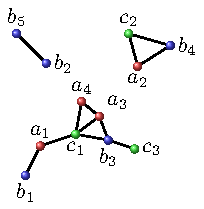
\includegraphics[width=0.3 \linewidth]{figures/spatialrelation.pdf}
\caption{空间关系示意图}{Spatial relation illustration}
\label{fig:spaitalrelation}
\end{figure}
\begin{equation}
\label{eq:colation}
 R(a_1,b_1) \Leftrightarrow (distance(a_1,b_1)\le d)
\end{equation}

空间特征集代表了空间不同种类对象的集合,记为$F=\{f_1,f_2,\ldots,f_n \}$;每一个具体空间位置上的对象称之为空间实例;
空间实例集$I=\{I_1,I_2,\ldots,I_m\}$,如果有$\{R(I_j,I_k) | 1 \le j \le m, 1 \le k \le m\}$,称$I$为一个簇;
空间co-location模式是一组空间特征的集合$C$,其中$C\in F$,一个co-location模式$C$的长度称此co-location的阶(Order);如果簇$I$的
包含了co-location模式$C$中的所有特征,并且$I$中没有任何一个子集可以包含$C$中所有特征,那么称$I$就是co-location模式$C$的
一个行实例$row\_instance(C)$,co-location的所有行实例表示为一个表实例$table\_instance(C)$。

在图\ref{fig:spaitalrelation}中,空间特征集为$F=(A,B,C)\text{,而}\allowbreak (c_2,b_4,a_2),\allowbreak (a_3,c_1,b_3)\text{,} \allowbreak (a_1,b_1) \text{,} \allowbreak (a_1,c_1)\text{,} \allowbreak (c_1,a_4)\text{和}(b_3,c_3)$
表示为一个簇。$(A,B,C)$可以表示为一个co-location模式,$(a_2,b_4,c_2)\text{和}(a_3,c_1,b_3)$表示了该co-location的行实例,
所有的行实例将组成表实例。

参与率和参与度是衡量co-location模式挖掘中重要参数,反映了一个空间模式的频繁程度。

(1)参与率

设$f_i$为某个空间特征,$f_i$在$k$阶co-location模式$C$中的参与率(participation ratio)表示为$PR(c, f_i)$,它是$f_i$的实例
在空间co-location模式$C$的所有不重复实例中不重复出现的个数与总实例的比例,定义见式\eqref{eq:participateratio}。
\begin{equation}
\label{eq:participateratio}
PR(c,f_i)=\frac{|\pi_{f_i}(table\_instance(c))|}{|table\_instance(\{f_i\})|}
\end{equation}

例如图\ref{fig:spaitalrelation}中,同位模式$(A,B,C)$所有的实例为$(a_2,b_4,c_2)\text{和}(a_3,c_1,b_3)$,空间特征$A$的实例对象
有$2$个$(a_2,a_3)$,而空间特征$A$的所有实例有$4$个$(a_1,a_2,a_3,a_4)$,所以$PR(\{A,B,C\},A)=2/4=0.5$;同理
$PR(\{A,B,C\},B)=2/5=0.4$,$PR(\{A,B,C\},C)=2/3=0.67$。

(2)参与度

co-location模式$c=\{f_1,f_2,\ldots,f_k\}$的参与度(Participation Index)表示为$PI(c)$,它是co-location
模式$C$的所有空间特征的$PR$值中的最小值,定义见式\eqref{eq:participateindex}
\begin{equation}
\label{eq:participateindex}
PI(c)=min_{i=1}^{k}\{PR(c,f_i)\}
\end{equation}

图\ref{fig:spaitalrelation}中,$PI(\{A,B,C\})=min(0.5,0.4,0.67)=0.4$。

$min\_prev$是需要给定的最小参与度阈值,只有当$PI(c) \ge min\_prev$时,称co-location模式$C$是频繁的。
co-location算法主要是基于最小参与度,由于最小参与度概念与Apriori算法相同的性质(向下闭合),很大程度上能降低
算法复杂度的开销,此类算法研究主要有:

\circled{1}Join-Based算法:一种基于完全连接的算法。该算法严格使用Apriori算法,$k$阶模式表之间通过连接(Join)操作
生成$k+1$阶候选者,对$k+1$表实例按照最小参与度筛选,该算法能够产生完整的co-location模式。

\circled{2}Partition-Join算法:一种基于部分连接的算法。该算法采用分治的思想,首先把空间所有按照距离阈值划分为不相交的实体块,
块与块之间实体不满足空间关联性,这样只需要进行块内部空间对象连接,大大降低了连接的计算量\cite{Yoo2004A}。算法的关键之处如何很好划分
出空间实体块,降低复杂度。

\circled{3}CPI-Tree算法:一种基于前缀树结构的无连接改进算法\cite{Wang2009Efficient}。该算法以前缀树表达空间实体对象之间的邻近关系,通过树结构
可以快速地处理表实例的增长,拥有较高的性能。但是如果数据量较大,存储和遍历树的代价将会增加,是一种折中的解决方案。

\subsection{Spatial-Spark同位模式}

全连接算法是一个依据先验原理,基于Join-Based操作产生候选模式和表实例的方法。主要流程分为以下两步:

(1)候选行实例生成

连接两个$k-1$个空间对象相同的频繁$k$阶模式实例表$P_{k1}$和$P_{k2}$,
生成$k+1$阶的候选行实例,在生成的过程中,检查行实例的所有对象是否满足空间距离阈值$d$。

(2)表实例的生成

根据所有候选行实例,按照每个行实例的模式进行汇总形成候选表实例,
对每个表实例计算所有特征的参与度,按照参与度过滤不满足阈值的表实例。

算法过程中,首先需要进行二阶模式行实例和表实例生成,算法时间复杂度将达到$O(n^2)$,当数据量急剧增加时候,
算法的时间消耗是不可接受的,需要进行并行化处理。借鉴Spatial-Spark计算框架中的空间连接运算,根据空间同位模式
的距离阈值$d$,将整个平面空间位置划分为均匀网格。以空间对象落入网格的横纵坐标编号作为
空间实体的Key,将所有空间实体生成Key-Value形式,见图\ref{fig:twoorder}中\uppercase\expandafter{\romannumeral1}
所示,每个空间实体对象拥有唯一的坐标。
\begin{figure}
\centering
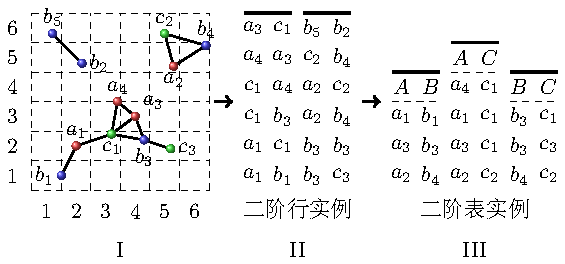
\includegraphics[width=0.8 \linewidth]{figures/two_order.pdf}
\caption{二阶模式生成}{Generation of 2 order location pattern}
\label{fig:twoorder}
\end{figure}

紧接着对所有实体对使用cogroup算子进行自相连,生成所有满足距离阈值的空间实体对,为了完整得获取所有空间邻近关系,
对坐横纵坐标差值绝对值不大于$1$的空间实体可判定为在可能存在邻近关系,
图\ref{fig:keyequal}中\uppercase\expandafter{\romannumeral1}, \uppercase\expandafter{\romannumeral2}
和\uppercase\expandafter{\romannumeral3}分别表示了三种相等情况。再使用filter算子进行过滤判断严格的邻近关系,
经过mapToPair操作生成所有的行实例,最后使用reduce操作按空间参与度过滤生成表实例。
\begin{figure}
  \centering
  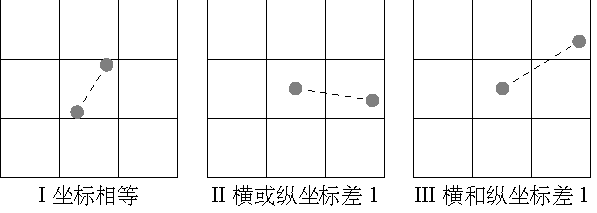
\includegraphics{figures/keyequal.pdf}
  \caption{坐标相等判断}{Judgement of coordinate equality}
  \label{fig:keyequal}
\end{figure}

图\ref{fig:twoorder}展示了完整的二阶生成模式流程,
\uppercase\expandafter{\romannumeral2}为列出所有行实例,\uppercase\expandafter{\romannumeral3}
则按照空间实体的特征进行汇总,按照参与度进行剪枝操作。
生成二阶模式后,根据同位模式的连接和剪枝步骤,生成更高阶数同位模式,见算法\ref{alg:colocaiton}。
% \begin{figure}
% \centering
% 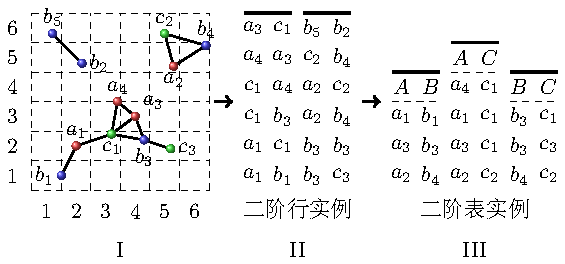
\includegraphics[width=0.8 \linewidth]{figures/two_order.pdf}
% \caption{二阶模式生成}{Generation of 2 order location pattern}
% \label{fig:twoorder}
% \end{figure}
\begin{algorithm}
\caption{co-location算法}
\label{alg:colocaiton}
\begin{algorithmic}[1]   
\REQUIRE  ~~\\  
点集:points;\\  
距离阈值:d;\\
参与度阈值:threshold;\\  
\ENSURE ~~\\  
空间同位模式:colocation patterns; \\
\STATE $P_2$ = Spatial-Spark.join(points, d, threshold)
\WHILE{$P_k$ is not empty and $k$ < N} 
\STATE $C_{k+1}$ = gen\_candinate\_cocolation($P_k$,$k$) $//$k+1阶候选集合
\STATE $C_{k+1}$ = pruning($C_{k+1}$, $d$) $//$剪枝处理
\STATE $T_{k+1}$ = gen\_table\_ins()$//$生成表实例
\STATE $P_{k+1}$ = Select\_Colocation\_Pattern($T_{k+1}$, threshold) $//$ 筛选表实例
\STATE $k$ = $k+1$ $//$下一轮迭代
\ENDWHILE 
\RETURN $P_2$,$\dots$,$P_k$
\end{algorithmic}  
\end{algorithm}

为了将不同的表实例进行连接操作,需要重写Join操作中key相等判断操作,定制了RowPattern类,重写equal方法,
当且仅当只有一个空间实例不等的时候,该行实例才相等。

RDD提供了Join操作,该操作对每个key下元素进行笛卡尔乘积,返回的结果再展平。当对$k$阶行实例进行join操作后,
对新加入的新添加的POI对象进行距离阈值$d$判断,获得有效的$k+1$阶行实例。以行实例的POI的类别Pattern为key进行
reduce操作生成表实例,按照参与率阈值进行剪枝操作,生成$k+1$阶表实例。设$k$阶模式$C1$和$k$阶模式$C2$连接得到$k+1$阶
候选模式$c3$,$C1$的行实例个数为$K1$,$C2$的行实例的个数为$K2$,$C3$的行实例个数为$K3$,在算法过程
中对$C1$和$C2$表进行连接操作,之后再$C3$表中进行查找,整个算法时间复杂度$O((k-2)K1\times K2 \times K3)$,实现
过程如下。
\begin{lstlisting}[language=Java][H]
while(colocations.count!=0){
  JavaPairRDD<RowPattern,Iterator<POI>> 
      rawRowInstances=colocations.join(colocations);
  JavaPairRDD<RowPattern,Iterator<POI>>
      validRowInstances=rawRowInstances.filter(
        //距离阈值判断
        distanceThresholdCheck();
      )
  JavaPairRDD<Pattern,Iterator<Iterator<POI>>>
      validTableInstance = validRowInstances.reduceBykey(
        //按pattern合并行实例
        combineRowInstances();       
      ).filter(
        //按照参与度进行剪枝
        participateratioCheck();
      );
  colocations=validTableInstance.mapToPair(
      //展开下一阶行实例
      flatRowInstances();
  )
}
\end{lstlisting}


\section{微博POI同位模式}{Co-Location Patterns in Weibo POIs}

微博用户签到地点是非常有趣的数据,反映了新浪微博用户在线下的活动情况,对现实生活的商圈发现、地点推荐
等重要的参考依据。POI空间模式挖掘中,为了过滤掉噪声信息,需要经过两步预处理:\circled{1}过滤签到数量较少的POI,
选择签到数量大于10的POI点;\circled{2}过滤POI所属类别不清楚,如「一般地点」、「楼宇」和「大门」等。

\subsection{二阶同位模式识别}
以不同的城市为研究区域,探索不同城市微博POI空间模式分布特征。选择空间距离阈值$d=500\text{\rm{m}}$,上海、武汉和
重庆三市微博POI类别二阶特征模式。由于新浪微博POI类别分类并非严格区分,比如「餐饮美食」与「中餐厅」存在着包含关系,因此
我们选择某一类别进行重点关注,比如选择「高等院校」在新浪微博POI中的与其他类别的同位关系及其空间参与度,
见表\ref{tab:advanceacademic}。
\begin{table}
  \centering
  \caption{高等院校二阶同位模式}{Advance academics' 2-order patterns}
  \label{tab:advanceacademic}
  \tabulinesep = 1.5mm
  \begin{tabu}to 1.0\linewidth{X[1,l,m]|X[1,l,m]| X[1,l,m]}
  \tabucline[0.1em]-
  \rowfont[c]{} 上海市 & 武汉市 & 重庆市 \\
  \tabucline-
  (高等院校,校园生活):0.556 &  (高等院校,校园生活):0.531 & (高等院校,校园生活):0.306 \\
  (高等院校,日本料理):0.472 & (高等院校,图书馆):0.528 & (高等院校,ATM):0.238 \\
  (高等院校,西餐厅):0.454 & (高等院校,糕饼店):0.384 & (高等院校,科研机构):0.224 \\
  (高等院校,甜品店):0.451 & (高等院校,快餐厅):0.368 & (高等院校,图书馆):0.224 \\
  (高等院校,培训机构):0.446 & (高等院校,四川菜):0.361 & (高等院校,超市):0.217 \\
  (高等院校,医院):0.443 & (高等院校,火锅店):0.358 & (高等院校,特色餐厅):0.215 \\
  (高等院校,糕饼店):0.441 & (高等院校,连锁酒店):0.354 & (高等院校,电子卖场):0.210 \\
  (高等院校,餐饮美食):0.432 & (高等院校,医院):0.328 & (高等院校,KTV):0.205 \\
  \tabucline[0.1em]-
  \end{tabu}
\end{table}

从表\ref{tab:advanceacademic}可以看出上海、武汉和重庆三市高等院校与周边同位模式POI类别差别不大,都是
与高校配套的相关服务类型,但是每个城市高等院校的周边类别差异较大。
由于上述三城市高等院校数量依次减少,因此相应的空间模式的空间参与度呈现下降趋势。

以(高等院校,培训机构)二阶模式为例,研究在不同空间距离阈值条件下在上述三市中空间参与度分布情况,
见图\ref{fig:participationIndexes},随着距离阈值增大,同位模式的空间参与度逐渐上升,而不
不同城市之间差异也非常明显。
\begin{figure}
  \centering
  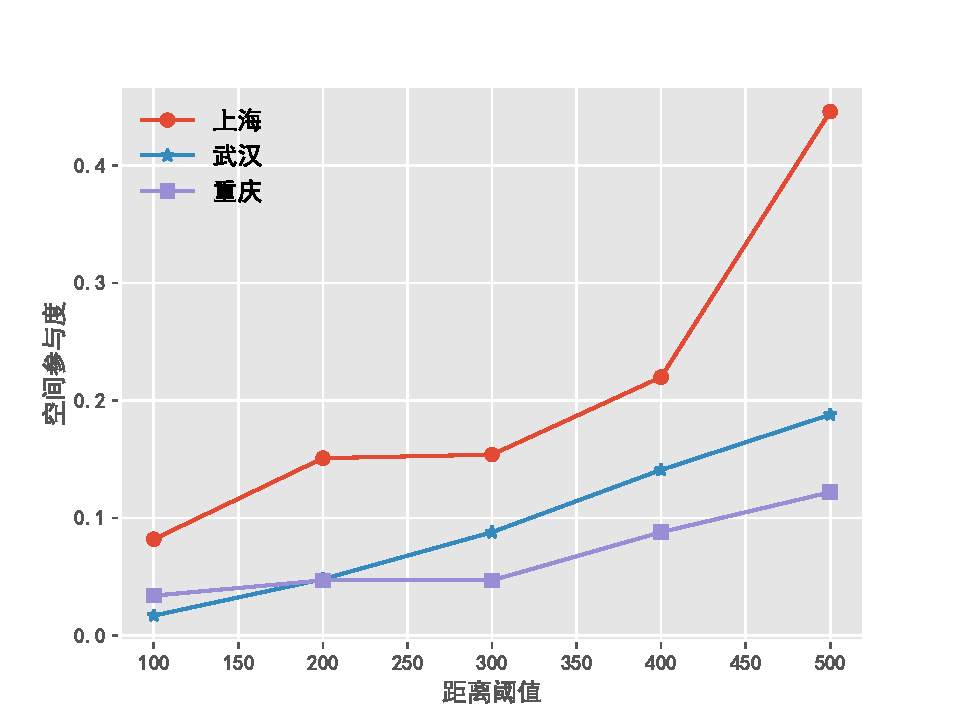
\includegraphics[scale=0.8]{figures/Participate.pdf} \\
  \caption{(高等院校,培训机构)模式不同距离阈值在不同城市空间参与度}{(Academic institutions \& Training institutions) Pattern's Paticipation indexes in different distances and cities}
  \label{fig:participationIndexes}
\end{figure}

\subsection{高阶同位模式识别}
北京市是全国新浪微博POI数量最多的城市,对该城市的新浪微博POI进行空间同位模式更具有代表性。在空间同位模式挖掘算法中,
连接距离阈值$d$和参与度阈值threshold是两个非常重要的,不同的参数将生成不同的空间同位模式,因此不同参数对北京市的POI进行
空间同位模式挖掘结果见表\ref{tab:distanceandthreshold}。
\begin{table}
  \centering
  \caption{不同距离和参与率空间同位模式}{Co-location patterns in defferent distances and PI's thresholds}
  \label{tab:distanceandthreshold}
  \tabulinesep=1.5mm
  \begin{tabu}to 0.8\linewidth{X[1.3,c,m]X[1.5,c,m]X[1,c,m]X[1,c,m]X[1,c,m]X[1,c,m]X[1,c,m]}
    \tabucline[0.1em]-
    距离\par 阈值 & 参与率 \par 阈值 & 2阶 & 3阶 & 4阶 & 5阶 & 6阶 \\
    \tabucline-
    \multirow{3}{*}{300} & 0.5 & 9 & 4 & 1 & - & - \\
     & 0.6 & 8 & 2 & - & - & - \\
    	& 0.7 & 5 & 1 & - & - & - \\
    \tabucline-
    \multirow{3}{*}{400} & 0.5 & 23 & 22 & 13 & 3 & - \\
     & 0.6 & 17 & 9 & 2 & - & - \\
     & 0.7 & 11 & 3 & - & - & - \\
    \tabucline-
    \multirow{3}{*}{500} & 0.5 & 40 & 40 & 26 & 11 & 2 \\
      & 0.6 & 29 & 29 & 19 & 7 & 1 \\
     & 0.7 & 22 & 17 & 7 & 1 & - \\
    \tabucline[0.1em]-
   \end{tabu}
\end{table}

通常来讲,距离阈值越大,参与率阈值越小,空间模式的生成阶越大,每一阶的模式数目越多。本文选择$d=500\text{\rm{m}}$,
参与度阈值为$0.6$,该参数既可以保留足够的细节信息,又能较好地反应空间分布的整体特征\cite{禹文豪2015设施},
新浪微博微博POI空间同位模式见表\ref{tab:poilocationpattern}。
\begin{table}
  \centering
  \caption{POI空间同位模式}{Co-location patterns of POIs}
  \label{tab:poilocationpattern}
  \tabulinesep=1.5mm
  \begin{tabu}to 1.0\linewidth{X[1,c,m]X[6,l,m]}
    \tabucline[0.1em]-
    \rowfont[c]{}  阶数 & 实例 \\
    \tabucline-
    二阶 &  (中餐厅,校园生活),(校园生活,医院),(甜品店,中餐厅),
            (咖啡厅,校园生活),(咖啡厅,酒吧),(清真餐馆,酒吧),
            (电影院,甜品店),(旅馆招待所,咖啡厅)$\ldots$  \\
    三阶 &  (中餐厅,校园生活,医院),(电影院,KTV,美容美发店),
            (甜品店,中餐厅,美容美发店),(美容美发店,酒吧,甜品店)
            (中餐厅,校园生活,咖啡厅)$\ldots$ \\
    四阶 & (电影院,KTV,咖啡厅,美容美发店),(KTV,中餐厅,甜品店,美容美发店),
            (甜品店,中餐厅,咖啡厅,美容美发店),(甜品店,咖啡厅,美容美发店,酒吧)$\ldots$ \\
    五阶  & (电影院,KTV,咖啡厅,甜品店,美容美发店),(KTV,中餐厅,咖啡厅,美容美发店,酒吧),
            (甜品店,中餐厅,咖啡厅,美容美发店,酒吧)$\ldots$ \\
    六阶 & (KTV,中餐厅,咖啡厅,甜品店,美容美发店,酒吧) \\
    \tabucline[0.1em]-
   \end{tabu}
\end{table}

通过对北京市新浪微博POI数据同位模式挖掘可以发现,同位模式阶数越高,POI模式越呈现商业模式,根据同位模式的「闭合性」,五
阶模式中的(电影院,KTV,咖啡厅,美容美发店),六阶模式中的(KTV,中餐厅,咖啡厅,甜品店,美容美发店,酒吧)在所有低阶模式中
全部出现,加上新浪微博POI是用户手动添加,这些地点在实体空间聚集性也反应了用户的集聚行为,因而这些对商业广告投放、商业
选址和商业促销等活动有很好的建议。

\section{本章小结}{Chapter Summary}

本章以新浪微博POI为研究重点,首先分析了如何快速地使用新浪微博API获取这些数据;然后使用统计分析,
得到了POI在签到数量和按类别统计信息,最后重点分析了如何使用Spatial-Spark对新浪微博POI数据同位模式
挖掘并行化设计,研究了上海、武汉和重庆二阶同位模式的特征,以北京为研究对象通过设定距离阈值和参与度阈值,
获取了该城市新浪微博POI空间同位模式,并得到一些结果,这些对商业决策有重要的参考意义。
\chapter{人口空间流动网络分析}{Analysis of Population Spatial Floating Network}
人口流动是直接塑造城市间关系的重要动力,也是城市发展活力指标\cite{甄峰网络社会}。城市之间的
人口流动研究始终是人文地理学、城市地理学和经济地理学所关注的热点。现代社会发展,交通网络的日趋
发达将城市发展与人口流动紧密地联系在一起,人口活动不再局限于一个封闭的城市。从全球、国家或区域
层面来看,人口流动已经跨越了地理的限制。传统的人口流动的统计方法费时费力,社交网络应用使用LBS功能
为研究这列问题提供了新思路,通过新浪微博提供的API接口获取特定时间段内全国范围内发送微博的用户,根据用户
的账户位置信息和发送微博的位置信息,构建基于社交地理的人口流动网络,如图\ref{fig:floatinpopulation}所示。
\begin{figure}
  \centering
  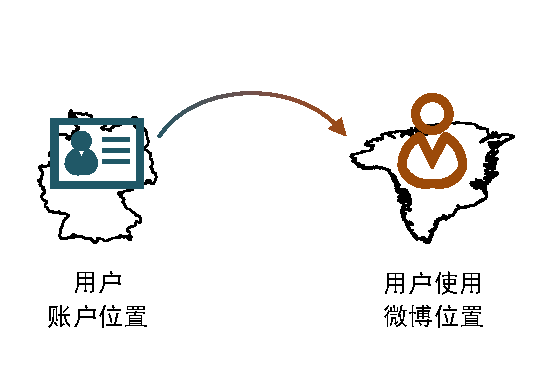
\includegraphics{figures/floating.pdf} \\
  \caption{流动示意图}{Floating illustration}
  \label{fig:floatinpopulation}
\end{figure}

\section{数据获取}{User Data Fetch}

新浪微博提供了place/nearby/users接口来获取附近发微博的用户,接口参数见表\ref{tab:poianduserapi}。
\begin{table}
  \centering
  \caption{NearbyUsers接口参数}{Nearby users api parameters}
  \label{tab:poianduserapi}
  \tabulinesep=1.5mm
  \begin{tabu}to 0.8\linewidth{X[1,c]X[1,c]X[2,c]}
    \tabucline[0.1em]-
    参数 & 类型 & 说明 \\
    \tabucline-
      lat & Float & 纬度 \\
      long & Float & 经度 \\
      starttime & Int64 & 开始时间 \\
      endtime & Int64 & 结束时间 \\
      range & Int & 查询半径,最大10km \\
    \tabucline[0.1em]-
   \end{tabu}
\end{table}

这些新浪微博用户数据包含了用户的名称、账号位置和用户当时所在空间位置,部分属性见格式见表\ref{tab:returnvalueuser}。
\begin{table}
  \centering
  \caption{用户地理空间位置(部分)}{Users' location information(partly)}
  \label{tab:returnvalueuser}
  \tabulinesep=1.5mm
  \begin{tabu}to 1.0\linewidth{X[1,c]X[2,c]|X[1,c]X[2,c]}
    \tabucline[0.1em]-
    属性 & 说明  & 属性 & 说明\\
    \tabucline-
    ID & 用户新浪微博ID & Name & 用户新浪微博名称 \\
    Province & 用户账户省份 & City & 用户账户城市 \\
    Lon & 用户位置经度 & Lat & 用户位置纬度\\
    \tabucline[0.1em]-
   \end{tabu}
\end{table}

春节前后是全国人口流动最为频繁的时间段,也是最能反映全国人口流动情况。因此选择$2016$年春节
前后$1$月$10$日和$2$月$10$日为起讫时间,获取全国微博用户位置数据,共$4.3$G,约$1500$万条用户记录。返回的数据为JSON格式,以键值的形式
保存表\ref{tab:returnvalueuser}中的属性,由于网络等其他问题,当请求量大的时候JSON数据中噪声较多,为了方便处理这些数据
因此将数据按行存放到HDFS中。

人口在不同城市之间流动构成了人口流动网络图,城市相当于网络图中节点,
不同城市之间人口流动相当于图中顶点之间的有向连接边,而人口流动数量则相当于边的权重。

GraphX作为Spark上层图处理模块,提供了并行化图分析算法。
为了方便分析城市人口流动分析,使用Spatial-Spark空间查询将全国数据抽象为一个Graph对象,
其中边$E_{ij}$为的权重为城市$j$中城市$i$用户的数量,算法流程图见\ref{fig:generateGraph}。
\begin{figure}
  \centering
  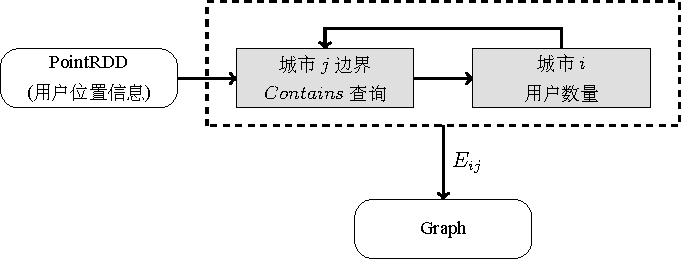
\includegraphics[scale=0.8]{figures/graph.pdf} \\
  \caption{Spatial-Spark生成人口流动网络图}{Generation floating population graph using Spatial-Spark}
  \label{fig:generateGraph}
\end{figure}

\section{人口流动统计}{Statistic of Floating Population}
\subsection{流动指数}

为了定量分析人口流动情况,定义如下指数:

\begin{description}
\item[流入量:]账户为其他城市在$i$城市发送微博的微博用户量,用$\delta_i$表示;
\item[流出量:]账户为$i$城市在其他城市发送微博的微博用户量,用$\omega_i$表示;
\item[流入流出比:]流入量/流出量,$\psi_i=\delta_i / \omega_i$。
\end{description}

\subsection{并行化设计}
GraphX丰富的图操作运算中\cite{Gonzalez2014GraphX},其中aggreateMessages是最核心最强大的接口,
该方法将边和其关联两个顶点作为一个Triplet进行整体并行处理,如图\ref{fig:triplet}所示,节点A和B以及它们之间的有向边
组成一个Triplet。首先进行类似map操作,将每个Triplet生成相应的消息,
发送关联的顶点,可以选择发送至目的节点,也可以选择发送至源节点;
然后对发送到同一个节点的消息进行reduce操作,进行合并操作。
\begin{figure}
  \centering
  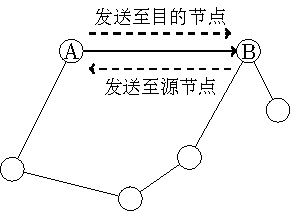
\includegraphics[width=0.4 \linewidth]{figures/triplet.pdf}\\
  \caption{Triplet操作示意图}{Triplet operations illustration}
  \label{fig:triplet}
\end{figure}

在计算城市人口流入量的时候,aggregateMessages接口中map操作选择将消息发送给有向边的目的节点;在计算城市
人口流出量的时候,map操作选择将消息发送给有向边的源节点,在reduce阶段所有消息汇总。
将上述两步生成的结果进行join和mapValue操作,计算每个城市的人口流动流出比,
算法流程见图\ref{fig:populationstatistic}。
\begin{figure}
  \centering
  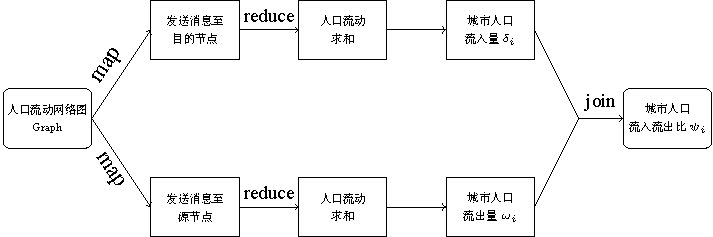
\includegraphics[width=0.9 \linewidth]{figures/population_statistic.pdf} \\
  \caption{人口流动统计流程图}{Flow chart of population statistic}
  \label{fig:populationstatistic}
\end{figure}

\subsection{统计分析}
以全国地级市和直辖市边界为空间查询范围,使用aggerateMessages函数分别计算出各自的流入量$\delta_i$、流出量$\omega_i$和流入
流出比$\psi_i$,结果栅格化渲染结果见图\ref{fig:flowinout}。
\begin{figure}
  \centering
  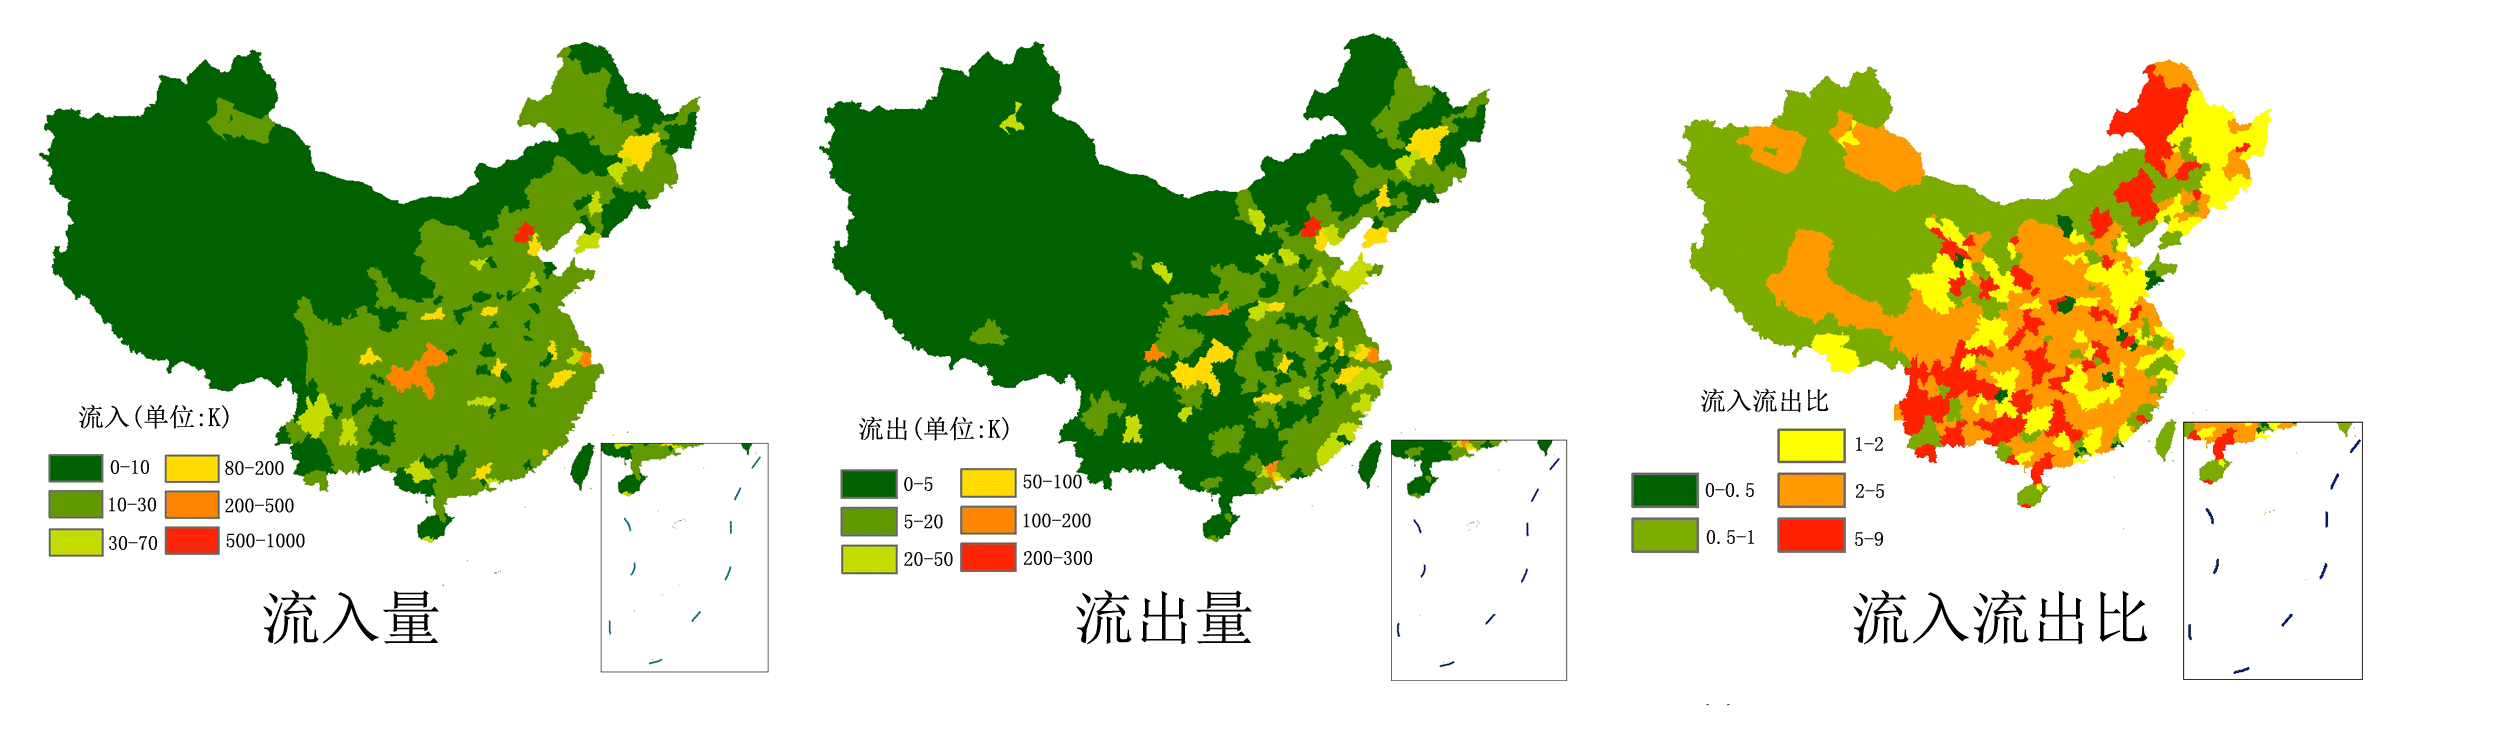
\includegraphics[width=13cm,height=4cm]{figures/flowratio.png} \\
  \caption{流出、流出和流入流出比}{Flow-in,flow-out and flow-ratio}
  \label{fig:flowinout}
\end{figure}

统计各个城市的人口流动数目,发现成都、西安、北京、广州、郑州等地为全国人口流动集中城市\cite{曹盼盼全国}。
并且人口流动量前$20\%$的城市占全国总用户的$70.1\%$,符合人口统计学和社会科学的「$80/20$法则」,
即$80\%$的事物或现象集中在前$20\%$的研究对象中。将前$20\%$城市人口流动统计见图\ref{fig:Populationstatistic},
可以看出人口流动流动量符合幂律分布(Power law)分布。
\begin{figure}
  \centering
  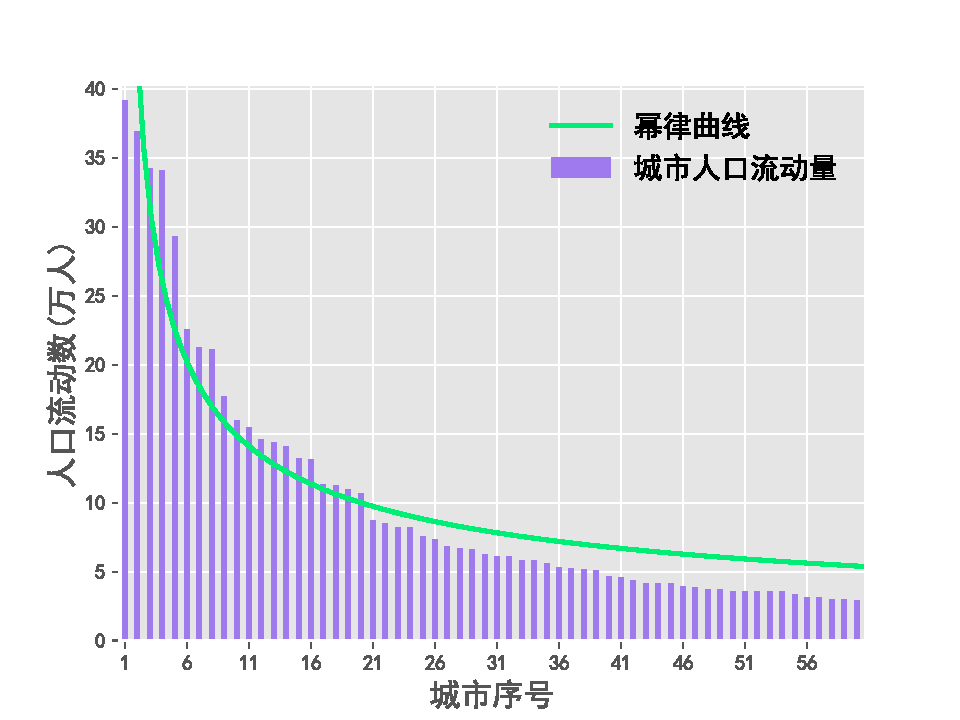
\includegraphics[scale=0.8]{figures/statisic.pdf} \\
  \caption{人口流动统计图}{Population flow statistic of cities}
  \label{fig:Populationstatistic}
\end{figure}

从图\ref{fig:flowinout}看出城市流入流出比呈现较多的复杂性:$\psi_i$远大于1表明该城市在春节期间人口呈现流入趋势;
$\psi_i$远小于$1$表明该城市在春节期间人口呈现流出趋势;而接近于$1$表明该城市人口在春节期间流动量持平,
主要城市的$\psi_i$见表\ref{tab:citiesinout}。
\begin{table}
  \centering
  \caption{城市流入流出比}{Cities' flow ratio}
  \label{tab:citiesinout}
  \tabulinesep=1.5mm
  \begin{tabu}to 1.0\linewidth{X[2,c,m]X[1,c,m]X[5,l,m]}
    \tabucline[0.1em]-
    \rowfont[c]{} 流入流出比$\psi_i$ & 说明 & 城市 \\
    \tabucline-
    大于1 & 流入 &   辽源、鄂州、西双版纳、毕节、永州、七台河、娄底、
                    姿阳、白色、黄冈、松原、三亚、娄底、大理等 \\
    接近1 & 持平 &  上海、北京、成都、武汉、哈尔滨、嘉兴、杭州、
                    长沙,广州、西安、太原、郑州、沈阳、乌鲁木齐等 \\
    小于1 & 流出 &  东莞、马鞍山、芜湖、青岛、苏州、深圳、包头、宁波、无锡、唐山,石家庄、呼和浩特等 \\
     \tabucline[0.1em]-
   \end{tabu}
\end{table}

流入流出比远大于$1$的城市主要有:\circled{1}春节返乡人群所在的城市,主要分布在人口劳动力输出的中西部城市,
四川、贵州、湖南、湖北等省份;剩余部分城市位于东北地区。\circled{2}南方著名旅游城市,海南,云南等省份。
随着旅游等第三产业发展,越来越多的人选择春节假期去度假,而不是回乡团聚,这些使得旅游城市在春节期
间迎来较大的人流量。

流入流出比接近$1$的城市春节期间人口流入量与流出量大致相同,这些城市主要是某个区域的连接中心,一般为省会城市,
如上海,北京,成都,武汉等等。

流入流出比小于$1$的城市主要有:\circled{1}沿海以劳动密集型产业发展起来的移民城市,集中在长三角和珠三角地区,据公安部最
新数据表明,深圳市常住人口超过$1300$万,但本地人口只有$250$万,外来人口超过$80\%$,位列全国第一,苏州以$50\%$外来人口排
名第二。\circled{2}重工业城市,其中以钢铁为代表重工业发展起来的城市如包头(包钢),唐山(首钢),马鞍山(马钢)等,人口
的流出可能与目前这些钢铁产业发达的城市产能过剩相关\cite{冯梅陈鹏钢铁}。

对人口流入流出比较大的城市,对这些城市交通、旅游等部门提供了决策依据,如航班的规划、旅游服务部门提前做好准备工作等等;也可以
通过从中人口的流入量,窥探城市经济走向和市场的活力。

\section{人口流向分析}{Analysis of Floating Population Route}

全国城市之间流动网络见图\ref{fig:citiesflow},从图中可以看出人口流向存在着不均衡性,明显的东部、中部和西部阶梯之分,
东部地区城市之间流动量大,流动密度强,中部地区次之而西部地区最小。
\begin{figure}
  \centering
  \includegraphics[scale=0.6]{figures/flow.jpg} \\
  \caption{城市人口流向}{Cities' population flow}
  \label{fig:citiesflow}
\end{figure}

\subsection{PageRank算法}
PageRank算法是Google搜索引擎的核心技术\cite{Boldi2009PageRank},该算法的核心思想
是将整个互联网抽象成网络图,每个网页抽象成一个节点,而节点之间的URL连接代表了网络图的边。
被许多重要页面引用的页面,往往还是重要的页面。算法开始假设所有节点拥有相同的权重,根据节点
的之间的链接权重设计出转移矩阵,通过权重转移矩阵相乘,重新分配权重,不停迭代循环,直至节点权重收敛。

以人口流动为例,将城市抽象成有向网络图中的各个节点,人口的流动抽象成节点之间的连通路径,构建出每个城市之间的流动矩阵$M$:

\[
  M=
\begin{bmatrix}
\alpha_{11} & \alpha_{12} & \ldots & \alpha_{1n} \\
\alpha_{21} & \alpha_{22} & \ldots & \alpha_{2n} \\
\ldots & \ldots & \ddots & \ldots \\
\alpha_{1n} & \alpha_{2n} & \ldots & \alpha_{nn} \\
\end{bmatrix}
\]

式中$\alpha_{ij}$为$i$城市人口流动至$j$城市的概率:
\begin{equation}
\label{eq:netprobability}
\alpha_{ij} = 
\left \{
  \begin{array}{cl}
  \frac{\beta_{ji}}{\sum_{k=0}^{k=n,k\ne i}\beta_{ki}} & i\ne j \\
  0 & i=j \\
  \end{array}
\right.
\end{equation}

式\eqref{eq:netprobability}中$\beta_{ki}$为在$k$城市微博用户中,账户位置为$i$城市的用户数量。
假设初始城市权重是相同的,即:
\begin{equation}
\label{eq:initalweight}
 V_0=
  \begin{bmatrix}
  1/n & 1/n & \ldots & 1/n 
  \end{bmatrix}^{T}
\end{equation}

通过$n$次迭代$V_n=M\times V_{n-1}$,直至$V_i$收敛,计算出每个城市在流动网络中的权重。

\subsection{城市流动网络权重}
GraphX模块中Graph类实现了PageRank算法,分为两种实现方式:一种是给定迭代次数的静态方法;另一种是给定
迭代收敛阈值的动态方法。本文选择动态方法,给定收敛阈值$0.0001$,计算得到权重前$20$位的城市见表\ref{tab:citiespagerank}。
\begin{table}
  \centering
  \caption{城市Pagerank排名}{Cities' Pagerank rank}
  \label{tab:citiespagerank}
  \tabulinesep=1.5mm
  \begin{tabu}to 1.0\linewidth{X[1,c]X[1,c]X[2,c]|X[1,c]X[1,c]X[2,c]}
    \tabucline[0.1em]-
    序号 & 城市 & PageRank值 & 序号 & 城市 & PageRank值 \\
    \tabucline-
    $1$ &   北京 & $0.058$ & $11$ & 厦门 & $0.014$  \\
    $2$ &   成都 & $0.033$ & $12$ & 哈尔滨 & $0.013$ \\
    $3$ &   上海 & $0.031$ & $13$ & 南京 & $0.012$ \\
    $4$	&   西安 & $0.028$ & $14$ & 长沙 & $0.012$ \\
    $5$ &   广州 & $0.026$ & $15$ & 沈阳 & $0.012$ \\
    $6$ & 	武汉 & $0.024$ & $16$ & 天津 & $0.011$ \\
    $7$ & 	杭州 & $0.017$ & $17$ & 长春 & $0.010$ \\
    $8$ & 	郑州 & $0.016$ & $18$ & 大连 & $0.009$ \\
    $9$ &	  深圳 & $0.015$ & $19$ & 济南 & $0.009$ \\
    $10$ &  重庆 & $0.014$ & $20$ & 太原 & $0.008$ \\
     \tabucline[0.1em]-
   \end{tabu}
\end{table}

以国家统计局2015年全国各直辖市、地级市和自治州的GDP数据,与城市人口流动网络权重进行相关性分析。
发现相关系数达$0.8$,表明呈现正相关关系,绘制散点图如图\ref{fig:rankgdpcorrelationanalysis}左
所示。为了更好的进行回归分析,将权重的平方根作为应变量,城市GDP数值作为响应变量,进行线性回归分析,结果如
图\ref{fig:rankgdpcorrelationanalysis}右所示,回归方程为:$\text{GDP} = 1.037\times 10^5 rank^{0.5}-2669$,
回归系数$\text{P-value} < 0.001$,通过假设检验。
\begin{figure}
  \centering
  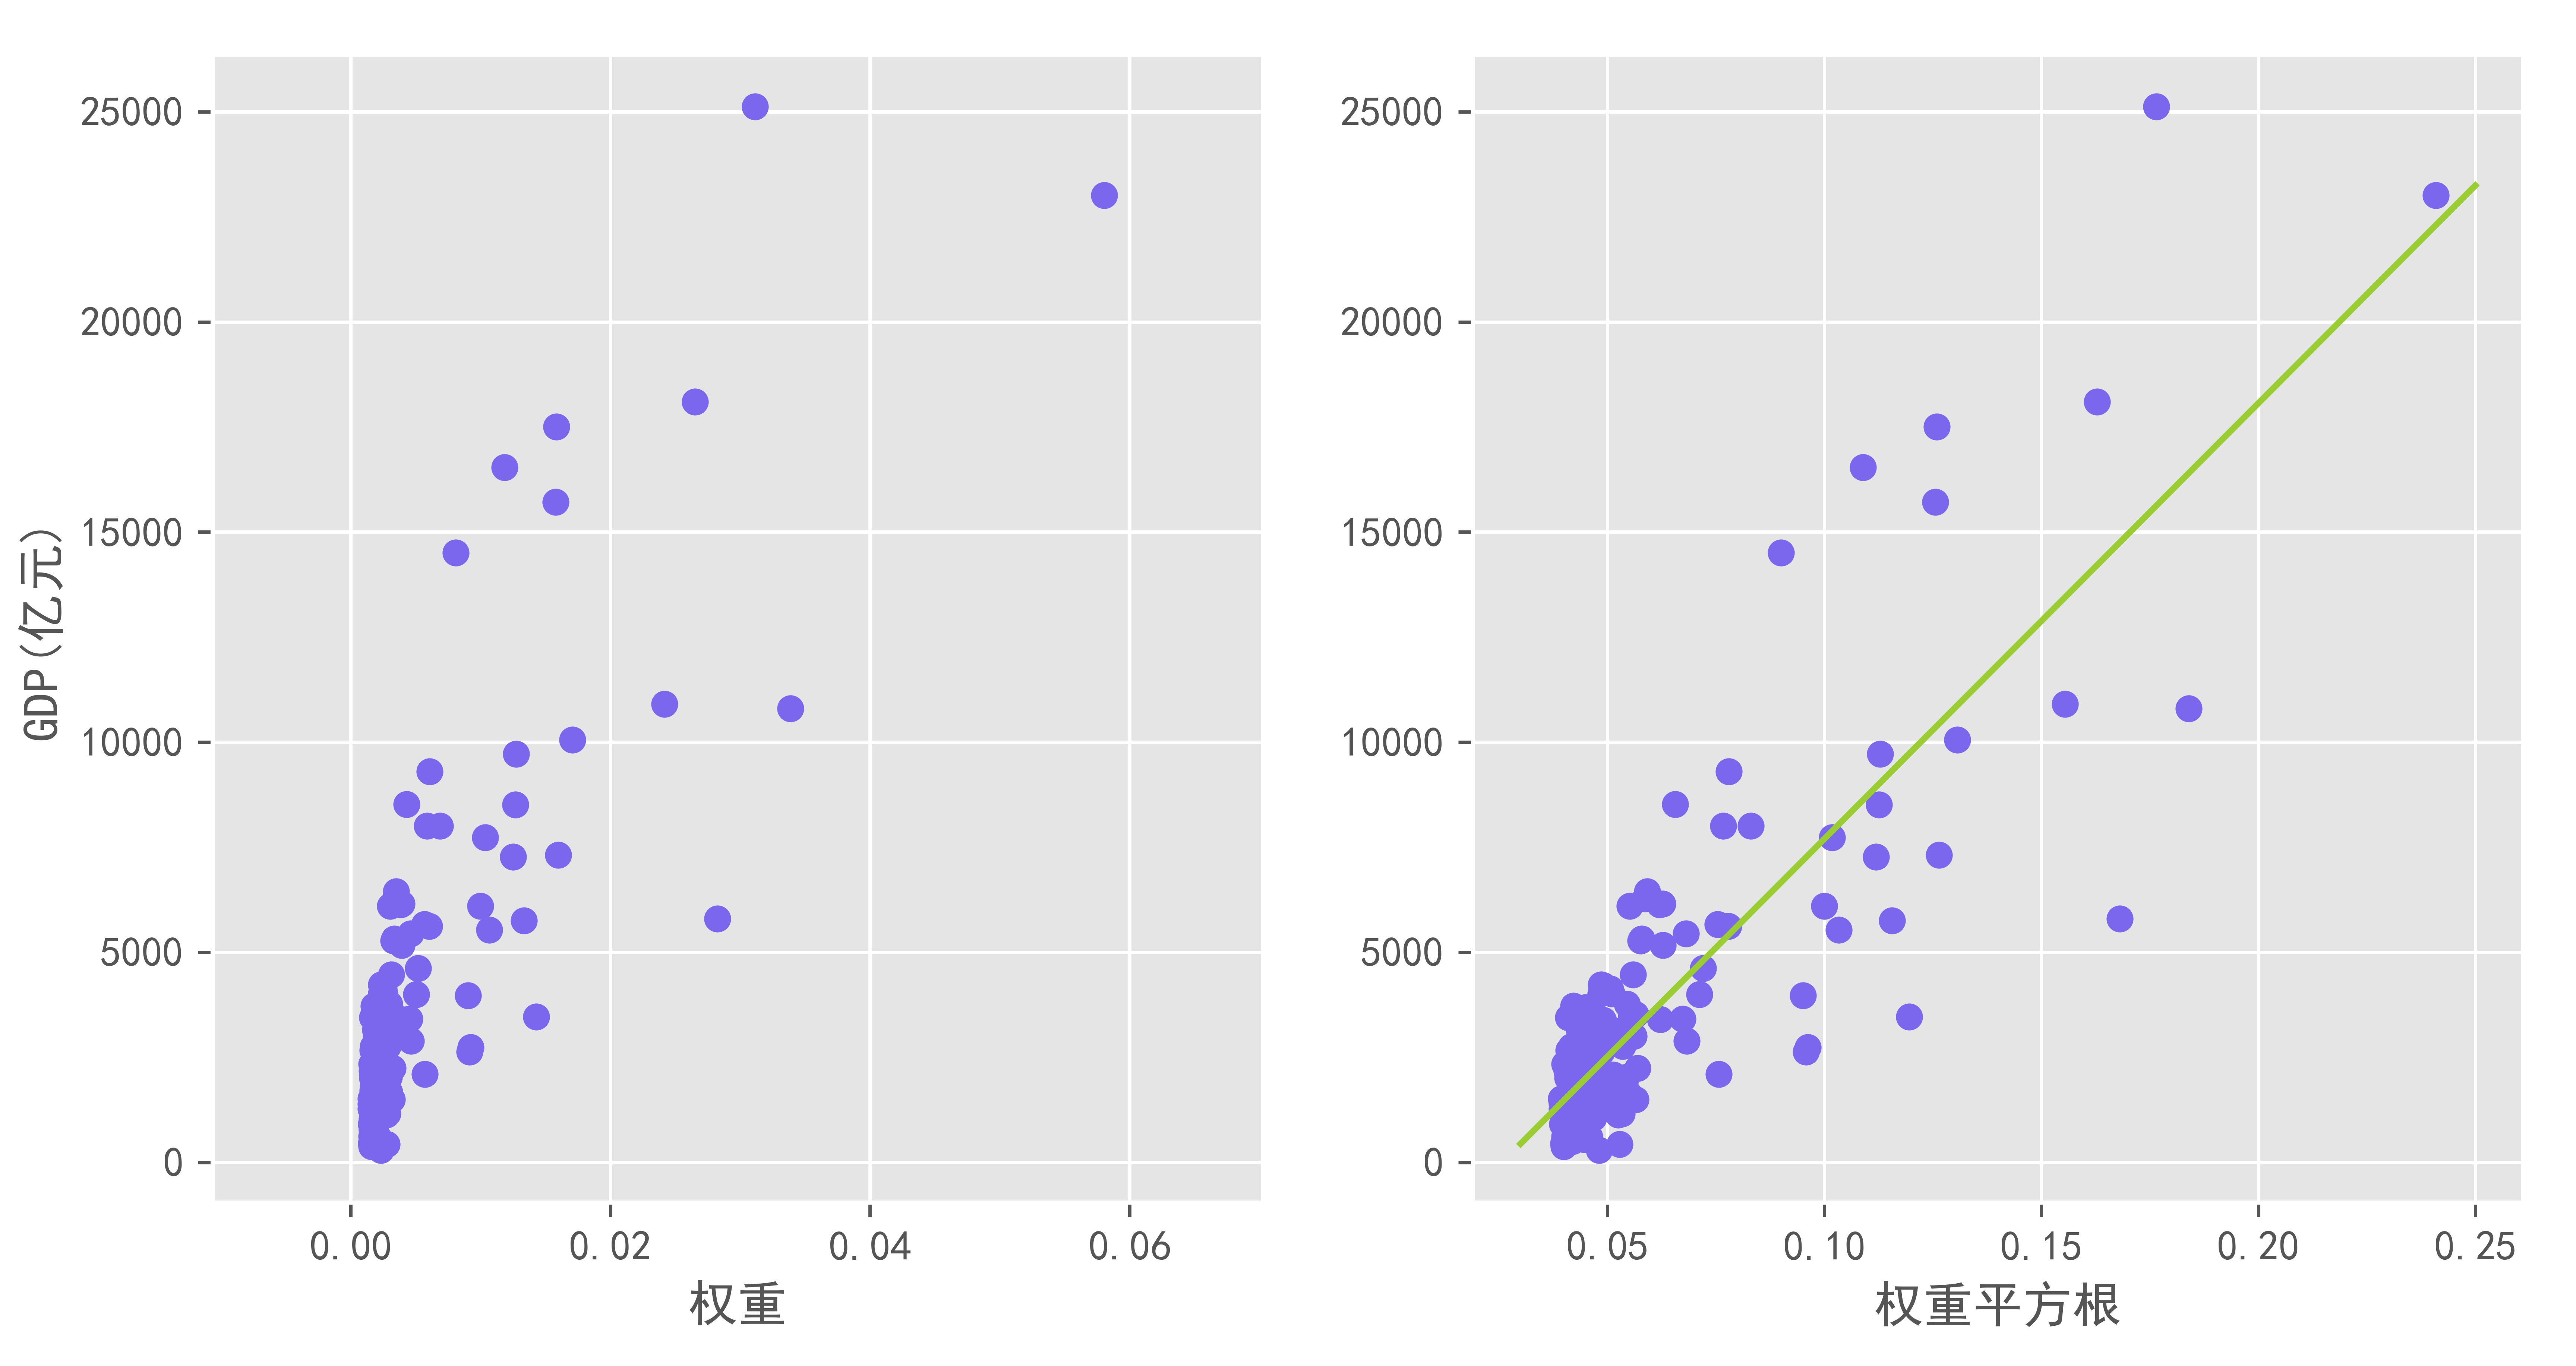
\includegraphics[scale=0.6]{figures/rank_gdp_scatter.png} \\
  \caption{权重和GDP相关性分析}{Ranks \& GDP correlation analysis}
  \label{fig:rankgdpcorrelationanalysis}
\end{figure}

从图\ref{fig:rankgdpcorrelationanalysis}中可以看出,并不是所有的点都很好的拟合回归曲线,存在「异常」
点。杠杆值可以描述点对整体回归的影响,高杠杆值可以说明改点属于异常点。据此绘制上述回归分析的残差平方与杠杆值散点图
,见图\ref{fig:residualLeverage},图中右下方和左上方的点属于异常点。
\begin{figure}
  \centering
  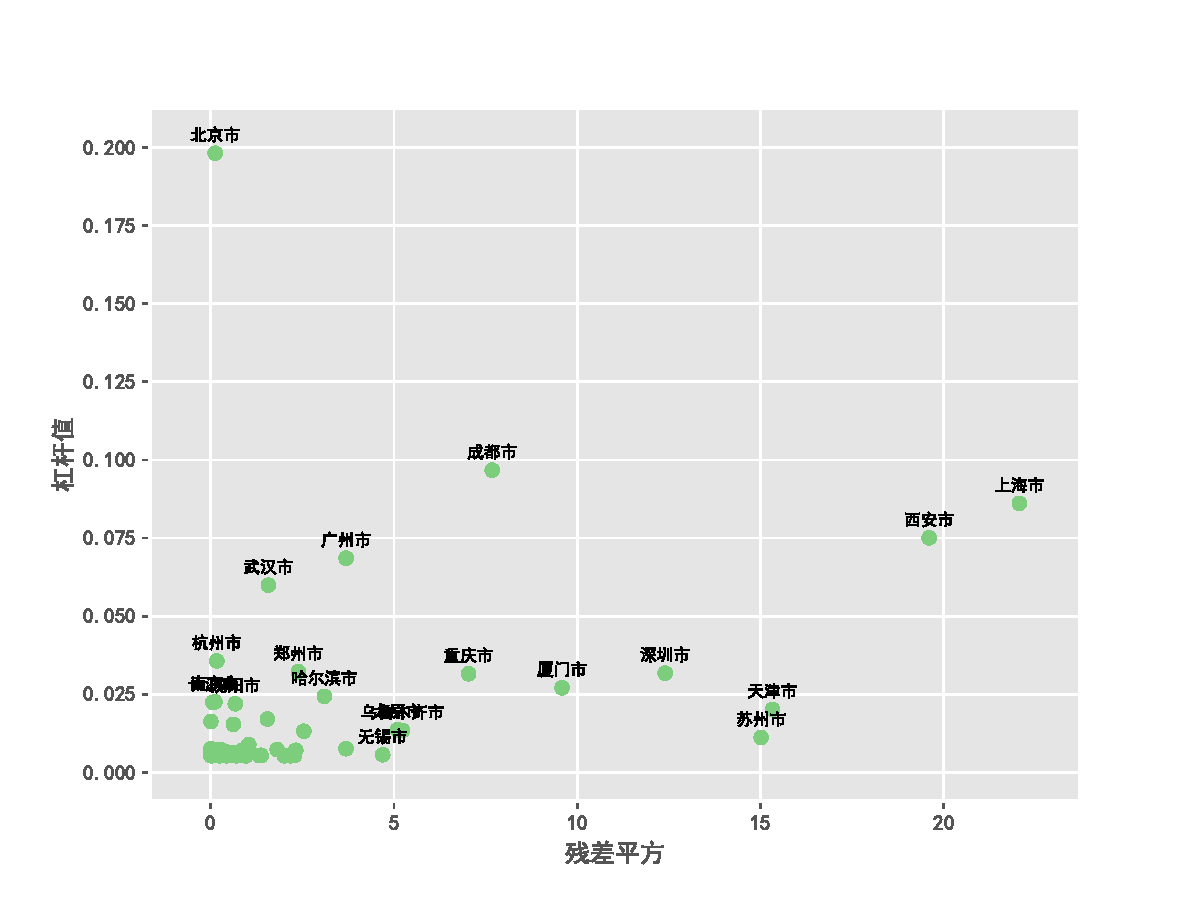
\includegraphics[scale=0.6]{figures/leverage.pdf} \\
  \caption{残差平方与杠杆值散点图}{Residual square \& leverage scatter plot}
  \label{fig:residualLeverage}
\end{figure}

城市特定时间段内在人口流动网络中的权重与实体城市权重存在明显的关系,出现了以下特征:

(1)城市权重与城市经济发展相对一致性。城市的权重与城市GDP呈现一定的正相关关系,
即城市的权重越高,城市的GDP数值会高。图\ref{fig:residualLeverage}中也表明了
在相关关系中异常点,主要分为两种:\circled{1}北京、成都、广州和武汉等城市权重
超出该城市GDP数值,其中北京最为明显;\circled{2}上海、西安、天津、苏州和深圳市等城市
的GDP发展远远大于该城市权重。

(2)城市权重在流动网络层级分布。通过对各个城市PageRank值分层,北京作为第一层级,是全国人口流动网络的中心;成都、上海、
西安、广州和武汉为第二个层级,是全国人口流动网络节点的副中心;杭州、郑州、深圳、重庆、厦门等为第三个层级,是区
域人口流动网络的中心;哈尔滨、南京、长沙、沈阳和天津等为第四个层级,是地区人口流动网络的中心。

(3)东部城市与中西部城市权重的差异明显。城市权重也符合「$80/20$法则」,排名前$20$城市权重和$0.81$。按照东部、中部、
西部三大地区划分,东部地区城市权重和$0.51$,中部地区城市权重和$0.32$,西部地区城市权重和$0.17$。虽然中部、西部地区也存在着权
重较高的城市,但东部区域在城市权重平均水平上明显高于中部和西部,因此东部城市在人口流动网络中扮演重要的角色。


\section{人口流动网络社群挖掘}{Community Mining of Floating Population Network}

现实世界中诸多系统都是以网络的形式存在,如人际关系网、机构协作网络、万维网等,这些统称为复杂网络(Complex Network),
可以通过简单的观测可以发现小规模网络的的特征、内部特征和划分,但是对于大规模和超大规模的网络,直观的显示很难通过肉眼发现
网络的特征和行为,因此需要使用复杂网络分析手段进行处理\cite{Girvan2002Community}。

网络社群挖掘(Community Mining,CM)是复杂网络聚类中研究最多的方法,社群挖掘方法对分析复杂网络中的拓扑结构,理解
复杂网络中隐藏的规律和预测复杂网络的行为不仅有重要的理论意义,而且有广泛的应用前景。城市之间人口流动也是属于一种复杂
网络,对该网络进行社群挖掘能够有效的发现城市在人口流动的联系,反映全国城市人口流动聚集效应。

\subsection{社群挖掘算法}

社群挖掘作为网络研究的经典问题,一直受到学者的广泛关注,目前社群挖掘算法主要有:GN(Girvan Newman)算法,定义边的介数,
依次删去介数最大的边,每次删除更新边的介数,如此循环,该算法在求解介数的时间复杂度较高\cite{Girvan2001Community};
LP(Label Propagation)算法使用邻居节点信息决定当前节点的社群,也可以应用到多社群挖掘,但是结果存在震荡问题,性能
不稳定\cite{Raghavan2007Near}。目前应用最多的是基于模块(Modularity)法,通过对比社群挖掘结果与随机图的差异判断社群划分的优劣,
研究表明基于模块值算法策略性能最好\cite{Newman2006Modularity}。

基于模块值算法通常先假设网络满足某种统计分布,进而通过极大似然估计方法得到网络社群。核心思想为模块值$Q$最大化,
见式\eqref{eq:qdefinition},$Q$是评价网络社群划分的优劣的质量指标。
\begin{equation}
\label{eq:qdefinition}
Q=\frac{1}{2m}\displaystyle{\sum_{vw}\big(W_{vw}-P_{vw}\delta(C_v,C_w)\big)}
\end{equation}

其中$W_{vw}$为网络中节点$v$和节点$w$之间的权重;$m$为权重之和;$P_{vw}$为零模型中节点之间的期望权重;$C_v$表示节点$v$所属的社群
的类别,如果节点$v$和节点$w$所属同一个社群,则$\delta(C_v,C_w)$为1,否则为0。

模块法开始将每个节点视为$N$个独立社群,选择使$Q$值增大最多或减少最小的连个顶点进行社群合并。
例如$A,B$连个社团合并,$a_i$为社团$A$中的成员,$b_j$为社团$B$中的成员,合并后的$Q$的
改变量用$\Delta Q$表示公式\eqref{eq:updateQ},$\Delta Q$为一个矩阵,其元素$e_{ij}$为社团$i$和
社团$j$合并后$Q$的变化值。%则社团合并后,因为合并无边相邻的社团对不能导致$Q$的增加,只需要考虑哪些相互之间有边的社团对。
\begin{equation}
\label{eq:updateQ}
\Delta Q_{AB}=Q_{AB}-Q_{A}-Q_{B}=\frac{1}{2m}\displaystyle{\sum_{a_i \in A, b_j \in B}}\bigg\{ \big( A_{ij} - \frac{k_ik_j}{2m} 
   \big) \times \delta \big[ r(i),r(j) \big] \bigg\}
\end{equation}

合并之后,对应的$\Delta Q$矩阵元素$e_{ij}$需要更新,如果选择让$A,B$社团合并为社团$D$,则新的社团$D$与其他社团之间(如社团$C$)
。在计算新一轮的合并$Q$时,易知$\Delta Q_{DC}=\Delta Q_{AC}+\Delta Q_{BC}$,上一次的迭代计算可以被
下一轮计算所采用,只需将$Q$矩阵中的$i,j$社团相关的行列相加,最多进行$n-1$次
计算来构建完整的社群划分\cite{Newman2012Communities}。

\subsection{社群挖掘算法并行化实现}

传统基于模块值社群挖掘算法是采用串行实现:逐个选择节点,选择合并社群,选择模块值最大的合并社群。而且需要两两考虑到
每个节点是否属于同一社群,算法时间复杂度将达到$O(n^2)$,当数据量急剧增加的时候,算法的时间消耗是可不接受的。因此
在并行计算框架下进行基于模块值进行社群挖掘,需要对公式\eqref{eq:qdefinition}简化为公式\eqref{eq:qdefinitionSimplify}。
其中$\sum_{in}$是社群$c$内部相互连接权重和,$\sum_{tot}$该社群$c$外部连接权重和。通过对比可以发现去掉了节点是否属于同一社群的判断
,避免了节点两两判断,简化了计算\cite{Blondel2008Fast}。
\begin{equation}
\label{eq:qdefinitionSimplify}
Q=\sum_{c}\big\{\frac{\sum_{in}}{2m} - (\frac{\sum_{tot}}{2m})^2\big\}
\end{equation}

判断某个节点$i$划分到其邻居节点计算模块值增益函数见公式\eqref{eq:updateQsimplify},其中$k_{i,in}$为节点$i$与社区$C$连接权重总和,
$k_i$为节点$i$与其余节点连接权重。
\begin{equation}
\label{eq:updateQsimplify}
\Delta Q=\big[ \frac{\sum_{in} + k_{i,in}}{2m} -(\frac{\sum_{tot}+k_i}{2m})^2 \big] 
      - \big[ \frac{\sum_{in}}{2m} - (\frac{\sum_{tot}}{2m})^2 - (\frac{k_i}{2m})^2 \big]
\end{equation}

算法主要分为两个步骤,第一步计算每个节点按照公式\eqref{eq:updateQsimplify}确定顶点$i$模块值增益最大进行合并社群,
第二步骤更新网络图,步骤见算法\ref{alg:communityMining}。
\begin{algorithm}[htbp]
\caption{社群挖掘算法}
\label{alg:communityMining}
\begin{algorithmic}[1]
\REQUIRE ~~\\
网络图:graph; \\
最多迭代次数: maxIterations;\\
模块值变化阈值: modularityThreshold;\\
\ENSURE ~~\\
模块值最大社群图: graph; \\
\STATE 初始化$C_i,\{i=1, 2,\ldots , N\}$
\STATE iterate=0
\WHILE{changeRate<modularityThreshold || iteration < maxIterations}
    \STATE changeRate=0
    \FORALL{$i$ in graph.vertexs} 
    \STATE $Q_i=[\quad ]$
    \FORALL{$j$ in $i$ neighbors}
    	\STATE $Q_i$ += $\Delta Q(i,j)$ $//$计算模块值增益
    \ENDFOR
    \STATE $Q_{max}$=max($Q_i$)
    \IF {$Q_{max} > 0$}
    	\STATE graph=updategraph() $//$如果最大模块值增益大于零,合并顶点
	\STATE changeRate= $Q_{max}$
    \ENDIF
    \ENDFOR
 \STATE iterate += 1 \\
\ENDWHILE
\RETURN graph
\end{algorithmic}
\end{algorithm}

算法\ref{alg:communityMining}每次迭代过程中依次选择图中的节点,对节点的所有的邻居节点尝试进行合并,对模块值增益最大且大于零的节点
进行合并。但是这种计算方式不利于并行计算框架,而且Spark RDD是不可变的数据结构,每次合并社群就要生成新的Graph对象,内存消耗非常大。
因此选择每次迭代更新多个节点,通过Graph类的aggregateMessages函数同时对图的所有边及其相关的节点进行同时操作,因此需要定义map阶段的
消息,按照公式\eqref{eq:updateQsimplify}的变量,定义如下消息结构。
\begin{lstlisting}[
  language=Java,
  morekeywords={implements, Integer, Long},
]
public class CombineMsg implements Serializable{
  public Integer degree;//该顶点的权重
  public Long commumity;//该顶点所属社区编号
  public Long commumityTotalDegree;//该社群权重总和
  public Long neighborDegree;//目标社群的权重
  public Long neighborCommumnity; //目标社群的编号
  public Long neighborCommumityTotalDegree;//目标节点的社群总权重
  public Long edgeWeight;//节点与与目标社群之间权重
}
\end{lstlisting}

对于发送到同一节点的消息集合,使用公式\eqref{eq:updateQsimplify},选择模块值增益值最大且大于$0$社群连边进行合并。
合并完毕后生成的消息图包含了本次社群合并连接顶点,并与原图进行joinVertice操作,完成图的更新。

由于所有边是并行操作,会出现「社群归属延迟」问题,如图\ref{fig:communityDelay}比如顶点$1$所在社群$c1$与顶点$2$所在社群$c2$进行合并,
而社群$c2$与顶点$3$所在社群$c3$进行合并,那么将会导致在joinVertice操作时候,这些顶点成为孤立的顶点。
从拓扑结构来看,社群$c1,c2,c3$应该属于同一个社群,因此对依据模块值增益生成的消息图计算连通分量,
直接使用Graph对象调用connectedComponents函数即可,最后与原图进行joinVertice操作,完成图的更新,流程示意图见图\ref{fig:Communitycombine}。
\begin{figure}
\centering
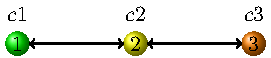
\includegraphics{figures/communitycombine.pdf}\\
  \caption{社群归属延迟}{Delay of commumity combine illustration}
  \label{fig:communityDelay}
\end{figure}

\begin{figure}
  \centering
  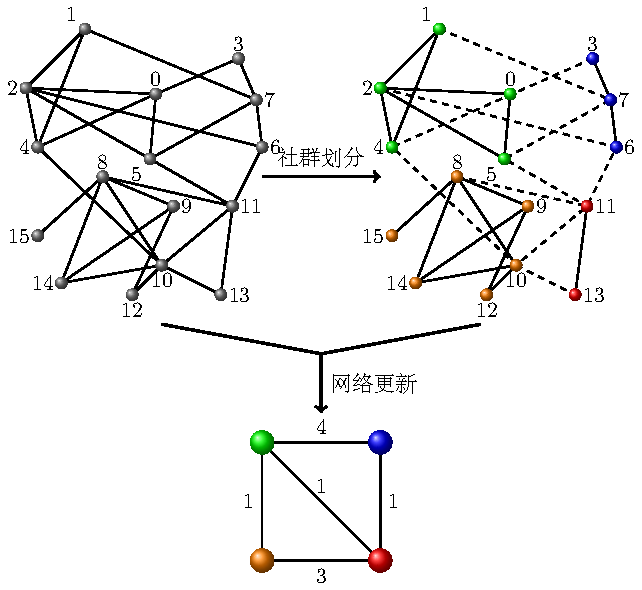
\includegraphics[scale=0.8]{figures/community.pdf}\\
  \caption{社群合并示意图}{Community combine illustration}
  \label{fig:Communitycombine}
\end{figure}

\subsection{城市社群挖掘}

由于人口流动往往存在较强的区域集聚性,在人口流动网络中体现出就是存在较强的社群结构,使用并行化
社群挖掘算法,反应全国城市人口流动的集聚效应\cite{杨小柳乡土中国}。对全国地级市和直辖市
人口流动网络进行社群挖掘,当整个人口流动网络划分为9个社群时,网络模块值最大,划分效果最好,
城市社群具体划分结果见图\ref{fig:nationalcommunitymining}和表\ref{tab:tbnationalcommunitymining}。
\begin{figure}
  \centering
  \includegraphics[width=10cm, height=8.115cm]{figures/commumity.jpg} \\
  \caption{全国城市社群划分}{National communities illustration}
  \label{fig:nationalcommunitymining}
\end{figure}
\begin{table}
  \centering
  \caption{全国城市社群划分详细}{National cities communities details}
  \label{tab:tbnationalcommunitymining}
  \tabulinesep=1.5mm
  \begin{tabu} to 1.0\linewidth{X[1,c,m]X[4,l,m]|X[1,c,m]X[4,l,m]}
    \tabucline[0.1em]-
    \rowfont[c]{} 社群&组成城市&社群&组成城市 \\
    \tabucline-
    1 & 北京、天津、河北城市、东三省城市、福建城市、三亚等 & 6 & 上海、江苏城市、安徽城市、浙江城市、丽江 \\
    2 & 山东城市 & 7 &广东城市、广西城市、湖南城市等\\
    3	& 河南城市	& 8	&重庆、四川城市、贵州城市等西南城市 \\
    4 & 山西城市 &	9 &	新疆城市、甘肃城市等西北城市 \\
    5	& 湖北城市、江西城市 & & \\
     \tabucline[0.1em]-
   \end{tabu}
\end{table}

对全国社群划分而言,也可以对其中的社群内部进一步使用社群挖掘算法,Spatial-Saprk强大的运算能力可以很容易的做到这一点,
比如上述全国社群1进一步使用社群挖掘算法,结果见图\ref{fig:subcommunity},每个社群中城市划见表\ref{tab:tabsubcommunity}。
\begin{figure}
  \centering
  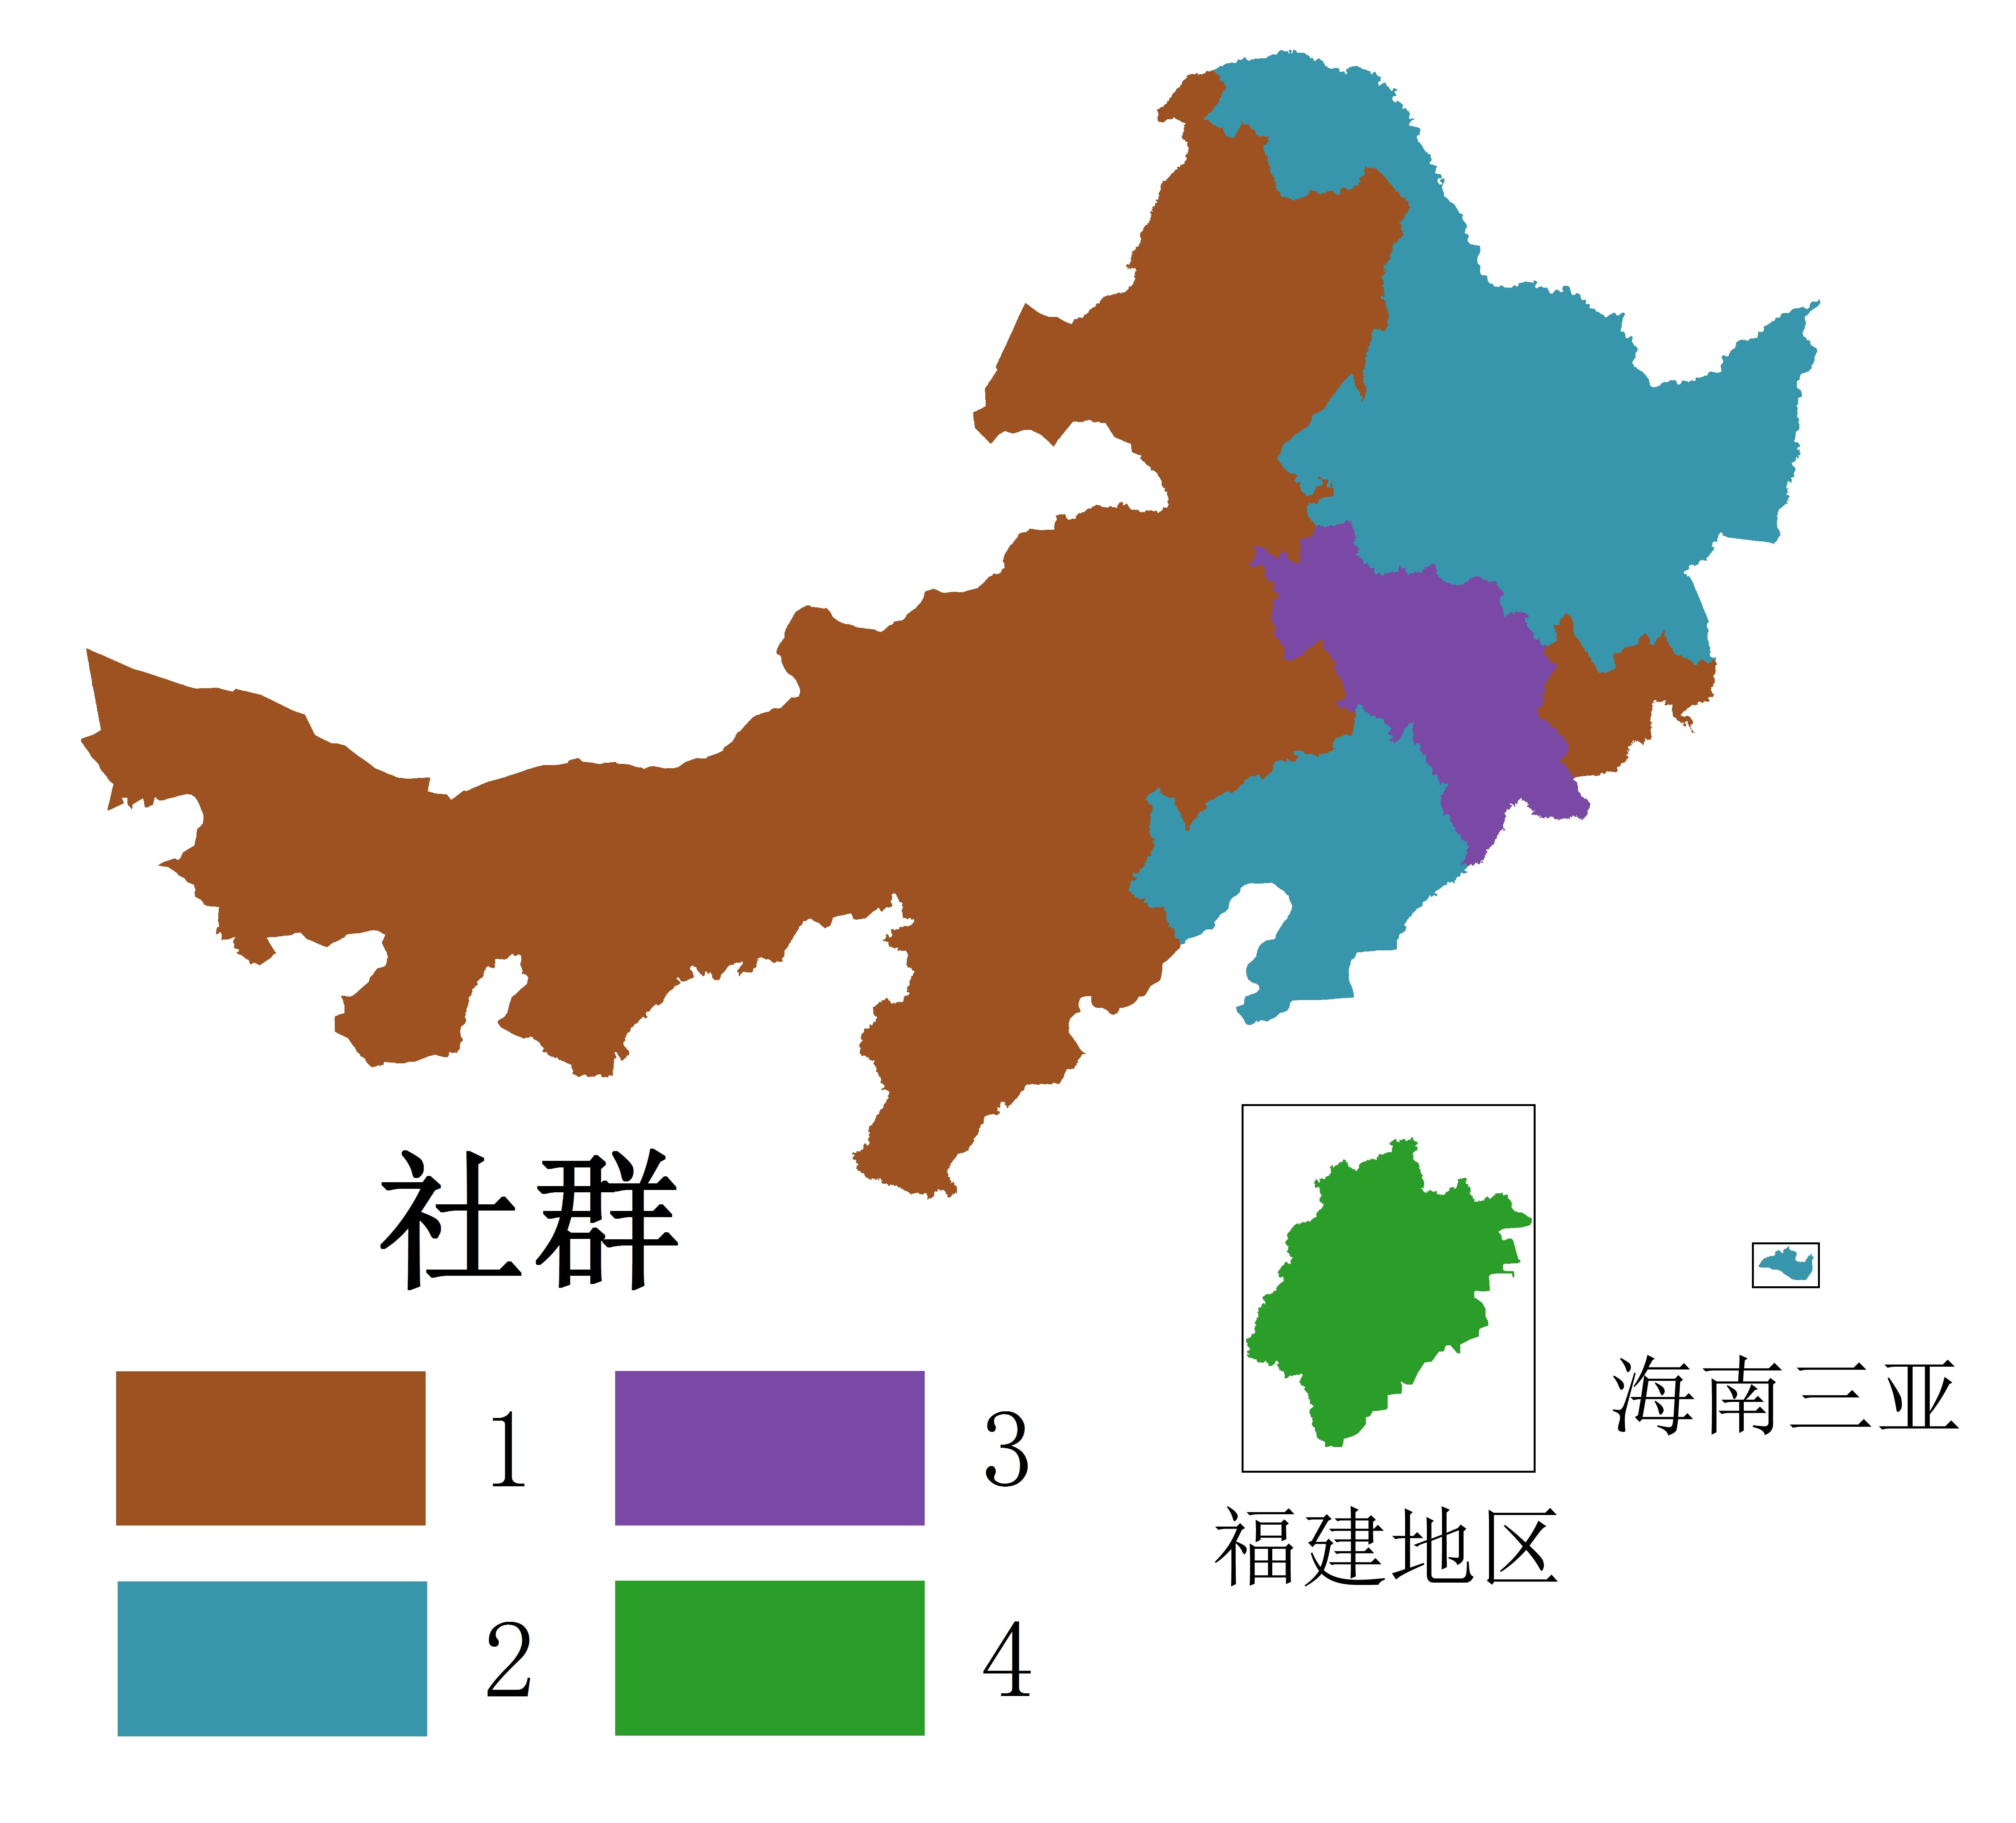
\includegraphics[width=8cm]{figures/subcommunity.jpg} \\ 
  \caption{子社群划分}{Sub-community illustration}
  \label{fig:subcommunity}
\end{figure}
\begin{table}
  \centering
  \caption{子社群划分}{Sub-community details}
  \label{tab:tabsubcommunity}
  \tabulinesep=1.5mm
  \begin{tabu} to 1.0\linewidth{X[1.2,c,m]X[6,l,m]|X[1.2,c,m]X[6,l,m]}
   \tabucline[0.1em]-
   \rowfont[c]{} 子社群 & 组成城市 & 子社群 & 组成城市 \\
    \tabucline-
   1 & 北京,天津,河北,内蒙古,吉林延边 & 2 & 黑龙江,辽宁,海南三亚 \\
   3 & 吉林城市 & 4 & 福建 \\
   \tabucline[0.1em]-
  \end{tabu}
\end{table}

分析每个社群的组成城市和城市之间地理空间分布,体现了以下特征:

(1)城市之间人口流动以省份为划分的特征较为明显,省份内部城市人口流动紧密
。以山东、山西、河南等省份为代表,其各自内部城市在人口流动网络中单独划分为一个社群。

(2)城市社群组成受地理空间位置影响较大,有明显的区域特征。在全国城市社群划分中,存在以北京为中心的
北方城市社群,上海为中心的东部城市社群,广东为中心的南部城市社群等集聚现象。

(3)城市社群组成也存在不受地理位置影响的特殊情况,如福建省的城市与北方城市组成同一社群,从侧面表
明其人口流动突破了地理空间的限制;丽江市与东部城市组成同一社群、三亚市与北方城市组成同一社群,
从一定程度表明这些旅游城市在春节假期的游客来源的组成。

(4)当对全国社群进行子社群进行社群挖掘,可以发现以省份为集聚现象越发明显,但是也可以发现少数城市与其他
省份人口联系更为密切,而这些往往是更值关注的内容,比如吉林的延边与北京、天津、河北等城市组成的社群更为
紧密,而海南三亚与黑龙江和辽宁组成的社群更为紧密。

通过对人口流动网络社群挖掘,可以快速地从海量数据中发现信息,这些信息既可以验证现实中已有的观念,如省份内部
人口流动紧密,空间邻近的省份人口交流频繁;也可以发现未知的现象,如福建省人口流动与北京、天津等省份城市
更为密切,海南三亚与北方城市尤其是黑龙江省份城市人口联系紧密。这些现象可以对省份和区域的决策者关于城市
规划、旅游航班调整、城市交通日常通勤等等方面提供很好的建议。

\section{本章小结}{Chapter Summary}

本章以全国新浪微博用户位置入手,构建了全国城市2016年全国城市人口流动网络,首先通过构建城市人口
流动指标,计算了城市人口流入、流出和流入流出比;借鉴PageRank计算每个城市在人口流动网络中的权重,
并与该城市GDP进行相关性分析,分析城市权重分布情况。最后对人口流动网络中进行社群挖掘,将全国城市
划分为9个社群,并分析了划分的特征。

\chapter{结论和展望}{Conclusion and Perspective}

\section{结论}{Conclusion}

为了高效处理海量空间数据,本文以Spark RDD为基础进行空间扩展,构建了
Spatial-Spark并行空间计算框架。以此框架为基础,对海量新浪微博空间数据进行有效
的分析,主要包括新浪微博POI数据和新浪微博用户位置数据分析和挖掘,并对
相关算法进行了并行化改进。

论文主要的工作及其成果总结如下:

(1)对Hadoop MapReduce和Spark并行计算框架进行分析,比较各自的优缺点。重点研究了
HDFS分布式存储策略和RDD的计算特点,分析Spark并行计算框架的优点,主要包括内存
计算带来的性能上优势和丰富的表现算子,为空间数据分析和挖掘提供了可能。

(2)以Spark为基础,对其进行空间方面的拓展,构建了并行空间计算框架Spatial-Spark,主要包括空间
数据分布式读写和空间数据变换,对基本的空间数据类型点、线和面分别拓展成为PointRDD、LineRDD
和PolygonRDD,并根据空间数据分布特征,提供了空间分区功能;
以R树为工具,对每个分区建立的空间索引,以加快空间数据分析速度。在此基础上,提供了
空间数据分析常用的模块,主要包含空间拓扑查询、KNN空间邻近查询和空间连接查询。最后搭建了分布式
Hadoop/Spark计算集群,验证了Spatial-Spark在空间数据处理方面的优势。

(3)分析了新浪微博提供的API接口,使用C\# SDK编写了获取新浪微博POI和全国新浪微博用户位置数据的
应用程序。

(4)研究了空间关联规则算法,重点分析了空间同位规则挖掘挖掘算,并结合Spatial-Spark提出了并行化
空间连接算法优化方案,对全国城市微博POI类别进行空位模式挖掘。首先针对上海、武汉和重庆三市进行
二阶模式挖掘,分析(高等院校、培训机构)模式在不同距离阈值下三市的空间参与度。选择空间距离阈值$d=500\text{\rm{m}}$和空间
参与度阈值$0.6$,对北京市进行同位模式挖掘,发现同位模式阶数越高,空间模式的数量越少,直至六阶,
(KTV,中餐厅,咖啡厅,甜品店,美容美发店,酒吧)为六阶空间模式的实例。由于新浪微博POI人为因素影响
较大,因此这些POI类别集聚的现象更加表达了现实线下人们活动现象,这对商家商业推广提供了很好的建议。

(5)新浪微博用户使用微博位置和用户账号位置形成人口流动,使用Spatial-Spark空间查询构建全国城市
在2016年春节期间人口流动网络图。首先根据GraphX并行计算功能,统计了各个城市人口流入量、流出量和流出
流出比,发现了全国城市人口流动情况的多样性;然后使用PageRank算法,计算出每全国城市在人口流动网络中
的权重并与城市GDP进行关联分析,发现城市权重与城市GDP发展相关联,并确定了各个等级区域人口流动网络的中心;
最后对整个人口网络进行进行社群挖掘,通过改进后模块值法,发现了全国城市人口流动社群,发现城市联系紧密性与省份有关,
地理位置对其影响很大,但也存在突破地理空间位置限制的城市。

\section{展望}{Perspective}

本文以新浪微博为研究内容,使用Spark进行了空间数据分析和挖掘进行了尝试,但是仍需在以下几个方面进行深入研究:

(1)空间连接分区索引使用:空间索引能有效地加快空间查询速度,但在Spatial-Spark上层空间连接模块中尚未有效
地使用已经建立的空间索引的进行加速算法,由于R树构造的特殊性,所以不能通过最小外包矩形进行Join操作。

(2)同位模式算法改进:在新浪微博POI类别同位模式挖掘中,使用全连接算法,虽然通过并行化改进在二阶模式
生成中减低了时间复杂度,但是在生成更高阶的过程中,RDD提供的join操作包含了较多的不满足条件的组合模式,因此
如果改进RDD在join操作的选择是值得研究的方向。

(3)微博数据获取方式改进:由于新浪微博API的限制性,不能获取关于用户的所有微博信息,因此在只能获取用户的
位置同时不能获取用户的历史微博数据,这些导致通过用户微博位置的注册地判断人口流动存在有偏性。如果采用网
络爬虫的方式,突破新浪微博API的限制,获取更多的用户的信息,那么将会发现更加有价值的信息。
\include{body/chap7}
\include{body/chap8}

\backmatter
\include{body/appendix}

\bibliographystyle{cumt}
\bibliography{RefExam}

\begin{resume}

\section*{一、基本情况}


姓名: \zuozhe\quad 性别: 男\quad 民族: 汉\quad 出生年月: 1992-02\quad 籍贯: 江苏扬州

2010-09 --- 2014-07\quad  中国矿业大学环境与测绘学院工学学士;

2014-09 --- 2017-06\quad  中国矿业大学环境与测绘学院工学硕士研究生.

\section*{二、学术成果}

\begin{enumerate}
  \item \zuozhe,土地确权内业处理软件,软件著作权,登记号:2015SR091014
\end{enumerate}


\section*{三、获奖情况}
\begin{enumerate}
  \item 2014-2015年度\quad 一等奖学金
  \item 2015-2016年度\quad 二等奖学金
  \item 2016-2017年度\quad 三等奖学金
\end{enumerate}
\section*{四、研究项目}
\begin{enumerate}
  \item 国家高分重点项目:中科院电子所苏州研究院, 2016, 参与;
  \item 国家自然基金项目:数字摄影测量目标精密定位于精度估计研究,编号:41171343, 参与;
  \item 山东省梁山县农村土地确权登记颁证项目,2014, 主要参与;
\end{enumerate}

\end{resume}

\GuanJianCi{\LaTeX; 模板; word; 使用说明; 格式; 表格; 图片}
\BingLieTiMing{\LaTeX{} 模板使用说明}
\LunWenYuZhong{中文}
\XueHao{ZS10080001}
\PeiYangDanWeiDaiMa{10}
\PeiYangDanWeiDiZhi{江苏省徐州市}
\XueZhi{三年}
\LunWenTiJiaoRiQi{2013 年 6 月}
\DaBianWeiYuanHuiChengYuan{戴朝寿, 江龙, 周圣武, 王海军, 李金玉, 范胜君}
%\LunWenZiZhu{}
%\XueWeiShouYuDanWeiMingCheng{}
%\XueWeiShouYuDanWeiDaiMa{}
%\XueWeiJiBie{}
%\LunWenTiMing{}
%\PeiYangDanWeiMingCheng{}
%\YouBian{}
%\XueWeiShouYuNian{}

\makebackcover
\printindex
\clearpage
\end{document}
